% LaTeX source for book ``代数学方法'' in Chinese
% Copyright 2024  李文威 (Wen-Wei Li).
% Permission is granted to copy, distribute and/or modify this
% document under the terms of the Creative Commons
% Attribution 4.0 International (CC BY 4.0)
% http://creativecommons.org/licenses/by/4.0/

% To be included
\chapter{单纯形方法}\label{sec:simplicial}
命 $\simpDelta$ 为非零有限序数范畴. 范畴 $\mathcal{C}$ 中的单纯形对象按定义是从 $\simpDelta^{\opp}$ 到 $\mathcal{C}$ 的函子 $X$, 它们也可以等价地描述为一列对象 $X_0, X_1, \ldots$ 及其间的态射 $d_i: X_n \to X_{n-1}$ (面) 和 $s_j: X_n \to X_{n+1}$ (退化), $0 \leq i, j \leq n$, 服从于一族等式 \eqref{eqn:simplicial-identity}; 这些函子构成范畴 $\cate{s}\mathcal{C}$. 对于 $\mathcal{C} = \cate{Set}$ 的特例, 它们也称为单纯形集. 相关的基本理论是 \S\S\ref{sec:simplicial-method}---\ref{sec:simplicial-set} 的内容. 命 $\cate{FinOrd}$ 为有限序数范畴, 若单纯形对象 $X$ 作为函子延拓为 $\cate{FinOrd} \to \mathcal{C}$, 则称之为增广单纯形对象, 这相当于在资料 $(X_n, d_i, s_j)_{n, i, j}$ 中添入 $-1$ 次项 $X_{-1}$.

单纯形集源于拓扑学, 想法是将空间剖分为单纯形的黏贴; 单纯形 (点, 线段, 三角形, 四面体...) 的直观图像是
\begin{center}\begin{tabular}{ccccc}
	$0$ 维 & $1$ 维 & $2$ 维 & $3$ 维 & $\cdots$ \\
	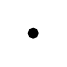
\begin{tikzpicture}[baseline=(P)] \fill[black] (0.5, 0.5) circle[radius=0.07]; \coordinate (P) at (0, 0.5); \end{tikzpicture} &
	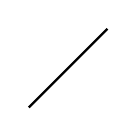
\begin{tikzpicture}[baseline=(P)] \draw[thick] (0,0) -- (1,1); \coordinate (P) at (0.5, 0.5); \end{tikzpicture} &
	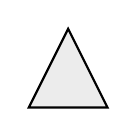
\begin{tikzpicture}[baseline=(P)] \filldraw[thick, fill=gray!15] (0,1) -- (-0.5, 0) -- (0.5, 0) --cycle; \coordinate (P) at (0, 0.5); \end{tikzpicture} &
	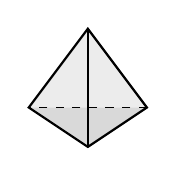
\begin{tikzpicture}[baseline=(P)]
		\fill[color=gray!15] (0, 1) -- (0.75, 0) -- (0, -0.5) -- (-0.75, 0) --cycle;
		\fill[color=gray!30] (0.75, 0) -- (0, -0.5) -- (-0.75, 0) --cycle;
		\draw[dashed] (0.75, 0) -- (-0.75, 0);
		\draw[thick] (0, 1) -- (0.75, 0) -- (0, -0.5) -- (-0.75, 0) --cycle;
		\draw[thick] (0, 1) -- (0, -0.5);
		\coordinate (P) at (0, 0.3);
	\end{tikzpicture} &
	$\cdots$
\end{tabular}\end{center}
依此对空间的同调和同伦等问题获取具体的, 或谓组合的理解. 此处采取的严格表述由 S.\ Eilenberg 和 J.\ A.\ Zilber 在 1950 年引入. 单纯形集的语言具有广泛的解释能力, 不限于经典的拓扑问题: 举例来说, 它能通过称为``脉''的构造来描述范畴, 详见 \S\ref{sec:nerves} 的介绍; 既然范畴论探讨图表中的对象 (表现为零维的点), 态射 (表现为一维的箭头) 和交换性 (关乎三角或方块等二维组件), 范畴和空间能统合于同一种数学结构之下并非意外.

在介绍脉和分类空间作为单纯形集的基本实例之后, \S\ref{sec:geom-realization} 回归直观, 定义单纯形集 $X$ 的几何实现 $|X|$; 定理 \ref{prop:geom-Sing-adjunction} 说明它和拓扑学家所熟悉的奇异集函子 $\mathrm{Sing}$ 一道构成伴随对
\[\begin{tikzcd}
	{|\cdot|}: \cate{sSet} \arrow[shift left, r] & \cate{Top} : \mathrm{Sing}. \arrow[shift left, l]
\end{tikzcd}\]
如以同伦论所常用的紧生成 Hausdorff 空间范畴 $\cate{CGHaus}$ 代替 $\cate{Top}$, 则几何实现还满足 $|X \times Y| \simeq |X| \times |Y|$, 左式的乘积是对两个单纯形集逐项取积; 证明关乎乘积的剖分, 其中一些组合学细节不尽平凡, 由于本书并非拓扑教材, 细节不深究.

相对于本书的主题, 更重要的是考虑 Abel 范畴 $\mathcal{A}$ 中的单纯形对象, 此时 $\cate{s}\mathcal{A}$ 也是 Abel 范畴; 例如单纯形 Abel 群构成 Abel 范畴 $\cate{sAb}$. 这方面的根本结果是 \S\ref{sec:Dold-Kan} 探讨的 Dold--Kan 对应 (定理 \ref{prop:Dold-Kan}), 它对 Abel 范畴 $\mathcal{A}$ 给出一对伴随等价
\[\begin{tikzcd}
	\Gamma: \cate{s}\mathcal{A} \arrow[shift left, r] & \cate{Ch}_{\geq 0}(\mathcal{A}): \mathrm{N}, \arrow[shift left, l]
\end{tikzcd}\]
其中 $\cate{Ch}_{\geq 0}(\mathcal{A})$ 代表 $\mathcal{A}$ 上的非负次链复形所成之 Abel 范畴. 函子 $\mathrm{N}$ 映单纯形对象 $X$ 为相应的正规化链复形 $\mathrm{N}X$; 更精确地说, 定义 $X \in \Obj(\cate{s}\mathcal{A})$ 的非正规化链复形为
\[ \mathrm{C}X := \left( X_n, \partial_n\right)_{n \geq 0}, \quad \partial_n := \sum_{i=0}^n (-1)^n d_i : X_n \to X_{n-1}, \]
则 $\mathrm{N}X$ 既可以按 $(\mathrm{N}X)_n := \bigcap_{i=1}^n \Ker(d_i)$ 取为 $\mathrm{C}X$ 的子链复形, 也可以理解为 $\mathrm{C}X$ 对退化部分的商, 两者之间的同构是命题 \ref{prop:Dold-Kan-v} 的内容; 事实上, 定理 \ref{prop:Dold-Kan-N-C} 说明嵌入态射 $u: \mathrm{N}X \to \mathrm{C}X$ 是链复形之间的拟同构.

Dold--Kan 对应使得单纯形理论不只在历史上, 而且在思想和技术两方面都成为同调代数的根源. 单纯形方法能够解释并升级复形或链复形上的基本操作, 例如同伦或可缩性质都有单纯形的版本, 从而获取拓扑诠释, 这部分讨论见诸 \S\ref{sec:homology-computation}.

另一种应用是搭配 \S\ref{sec:Beck} 的单子理论, 由此可以典范地将范畴中的对象扩充为相应的增广单纯形对象或增广余单纯形对象; 鉴于它们和 Hochschild 同调中的``加杠''操作有关, 这些技术统称为杠构造, 是 \S\ref{sec:bar-resolution} 的主题. 通过 Dold--Kan 对应和一些关于可缩性的观察, 杠构造解释了 Hochschild 理论 (见 \S\ref{sec:HH}) 和群上同调理论 (见 \S\ref{sec:G-mod}) 中的种种标准解消, 说明它们出于更高阶的奇思妙想. 习题包含关于杠构造的其他延伸内容.

按照定义, \S\ref{sec:bisimplicial} 讨论的双单纯形对象无非是函子 $\simpDelta^{\opp} \times \simpDelta^{\opp} \to \mathcal{C}$, 它们构成范畴 $\cate{s}^2 \mathcal{C}$. 对于取 $\mathcal{A}$ 为 Abel 范畴的情形, 与 $\cate{s}^2 \mathcal{A}$ 直接相关的 Eilenberg--Zilber 定理 \ref{prop:Eilenberg-Zilber} 是代数拓扑学中的基本构造; 纯粹从范畴论观点看, 在 $\mathcal{A}$ 为幺半范畴的前提下 (例如 $\mathcal{A} = \cate{Ab}$), 它为函子 $\mathrm{N}: \cate{s}\mathcal{A} \to \cate{Ch}_{\geq 0}(\mathcal{A})$ 提供了双向的典范幺半结构. 然而双单纯形对象的应用不止于此.

本章最后的 \S\ref{sec:closed-simplicial} 和 \S\ref{sec:mapping-cone-revisited} 分别探讨单纯形集的 $\Hom$ 对象和映射锥. 它们一方面对应到拓扑直观中的映射空间和锥, 另一方面又在 Abel 群情形通过 Dold--Kan 对应给出熟悉的 $\Hom$ 链复形和映射锥. 复形或链复形上的相应构造因此获得了明白的解释, 而拓扑学家对这一切如数家珍.

\begin{wenxintishi}
	本章的 \S\S\ref{sec:simplicial-method}---\ref{sec:geom-realization} 构成单纯形方法的主干, \S\S\ref{sec:Dold-Kan}---\ref{sec:bar-resolution} 和链复形直接相关, 而 \S\S\ref{sec:bisimplicial}---\ref{sec:mapping-cone-revisited} 尽管和本书先前的内容声气相通, 其属性则接近延伸内容. 相对于本书其他各章, 单纯形方法并非逻辑必需品, 然而其中的思想与技术属于数学工作者的基本素养, 更是踏入高阶代数的基础. 关于单纯形对象的一些论证有时涉及琐碎的验证 (如 \S\ref{sec:Dold-Kan}), 这是定义使然, 请读者酌情选择.
\end{wenxintishi}

\section{单纯形对象}\label{sec:simplicial-method}
我们在注记 \ref{rem:walking-algebra} 回顾了何谓偏序集之间的保序映射, 并且由之定义了有限序数范畴 $\cate{FinOrd}$. 本章聚焦于非零序数构成的全子范畴 $\simpDelta$.

\begin{definition}
	\index[sym1]{Delta-simp@$\simpDelta$}
	\index[sym1]{[n]}
	令 $\simpDelta$ 为所有有限非零序数及其间的保序映射构成的范畴. 换言之, 它的对象是全序集 $[n] := \{0, \ldots, n \}$, 其中 $n \in \Z_{\geq 0}$, 而态射是保序映射.
\end{definition}

请注意: 不应混淆 $[n]$ 与 $\mathbf{n}$, 后者在本书中代表全序集 $\{0, \ldots, n-1 \}$ 或相应的范畴.

范畴 $\simpDelta$ 中的任意态射 $[l] \to [n]$ 都能唯一地分解为保序满射和保序单射的合成
\[ [l] \twoheadrightarrow [m] \hookrightarrow [n], \quad n \geq m \leq l, \]
而如上的单射 (或满射) 又可以拆成片段, 使得每步恰好遗漏一个元素 (或恰好简并两个元素); 换言之, 所有态射都能分解为下述两类态射的合成.
\begin{center}\begin{tabular}{|c|l|l|l|} \hline
	余面 & $\mathrm{d}^i = \mathrm{d}^{n, i}: [n-1] \hookrightarrow [n]$ & $0 \leq i \leq n$ & 仅遗漏 $i \in [n]$ 的保序单射 \\ \hline
	余退化 & $\mathrm{s}^j = \mathrm{s}^{n, j}: [n+1] \twoheadrightarrow [n]$ & $0 \leq j \leq n$ & 取两次 $j \in [n]$ 的保序满射 \\ \hline
\end{tabular}\end{center}

一个保序单射 (或满射) 可按多种方式分解为余面 (或余退化), 取决于遗漏 (或简并) 元素的次序. 以下的\emph{余单纯形等式}的验证毫无困难:
\begin{equation}\label{eqn:cosimplicial-identity}\begin{array}{ll}
	\mathrm{d}^j \mathrm{d}^i = \mathrm{d}^i \mathrm{d}^{j-1}, & i < j, \\
	\mathrm{s}^j \mathrm{d}^i = \mathrm{d}^i \mathrm{s}^{j-1} & i < j, \\
	\mathrm{s}^j \mathrm{d}^j = \identity = \mathrm{s}^j \mathrm{d}^{j+1}, & \forall j, \\
	\mathrm{s}^j \mathrm{d}^i = \mathrm{d}^{i-1} \mathrm{s}^j, & i > j+1, \\
	\mathrm{s}^j \mathrm{s}^i = \mathrm{s}^i \mathrm{s}^{j+1}, & i \leq j.
\end{array}\end{equation}

仔细思考保序单射 (或满射) 的不同分解方式之间如何过渡, 可见余面, 余退化和 \eqref{eqn:cosimplicial-identity} 实则为 $\simpDelta$ 的态射结构给出了完整的生成元和关系.

改置于 $\simpDelta^{\opp}$ 中考量, 相应地便有态射
\begin{center}\begin{tabular}{|l|l|l|} \hline
		面 & $\mathrm{d}_i = \mathrm{d}^n_i: [n] \xrightarrow{\opp} [n-1]$ & $0 \leq i \leq n$ \\ \hline
		退化 & $\mathrm{s}_j = \mathrm{s}^n_j: [n] \xrightarrow{\opp} [n+1]$ & $0 \leq j \leq n$ \\ \hline
\end{tabular}\end{center}
符号 $\xrightarrow{\opp}$ 只为提示箭头属于相反范畴 $\simpDelta^{\opp}$. 将 \eqref{eqn:cosimplicial-identity} 倒转, 可得\emph{单纯形等式}
\begin{equation}\label{eqn:simplicial-identity}\begin{array}{ll}
	\mathrm{d}_i \mathrm{d}_j = \mathrm{d}_{j-1} \mathrm{d}_i, & i < j \\
	\mathrm{d}_i \mathrm{s}_j = \mathrm{s}_{j-1} \mathrm{d}_i & i < j \\
	\mathrm{d}_j \mathrm{s}_j = \identity = \mathrm{d}_{j+1} \mathrm{s}_j, & \forall j \\
	\mathrm{d}_i \mathrm{s}_j  = \mathrm{s}_j \mathrm{d}_{i-1}, & i > j+1 \\
	\mathrm{s}_i \mathrm{s}_j = \mathrm{s}_{j+1} \mathrm{s}_i, & i \leq j.
\end{array}\end{equation}
\index{danchunxingdengshi@单纯形等式 (simplicial identities)}

\begin{definition}\label{def:simplicial-obj}
	\index{danchunxingduixiang@单纯形对象 (simplicial object)}
	\index{yudanchunxingduixiang@余单纯形对象 (cosimplicial object)}
	\index{danchunxingduixiang!增广 (augmented)}
	\index[sym1]{sC@$\cate{s}\mathcal{C}, \cate{cs}\mathcal{C}$}
	给定范畴 $\mathcal{C}$,
	\begin{itemize}
		\item 其中的\emph{单纯形对象}意谓函子 $\simpDelta^{\opp} \to \mathcal{C}$, 全体单纯形对象构成范畴 $\cate{s}\mathcal{C} := \mathcal{C}^{\simpDelta^{\opp}}$;
		\item 其中的\emph{余单纯形对象}意谓函子 $\simpDelta \to \mathcal{C}$, 全体余单纯形对象构成范畴 $\cate{cs}\mathcal{C} := \mathcal{C}^{\simpDelta}$.
	\end{itemize}

	因此 $(\cate{cs}\mathcal{C})^{\opp} \simeq \cate{s}(\mathcal{C}^{\opp})$. 如果一个单纯形对象 (或余单纯形对象) 带有到 $\cate{FinOrd}^{\opp}$ (或 $\cate{FinOrd}$) 的延拓, 则称之为\emph{增广}的.
\end{definition}

\index[sym1]{di@$d_i, \mathrm{d}_i$}
\index[sym1]{sj@$s_j, \mathrm{s}_j$}
基于先前的讨论, 指定单纯形对象 $X$ 相当于指定 $\mathcal{C}$ 的一族对象 $(X_n)_{n \geq 0}$ 连同一族满足 \eqref{eqn:simplicial-identity} 的态射
\[ d_i = d^n_i: X_n \to X_{n-1} \; \text{(面)}, \quad s_j = s^n_j: X_n \to X_{n+1} \; \text{(退化)}, \quad 0 \leq i, j \leq n. \]
我们称 $X_n$ 为 $X$ 的 $n$ 次项. 从单纯形对象 $X$ 到 $Y$ 的态射相当于 $\mathcal{C}$ 的一族态射 $(f_n: X_n \to Y_n)_{n \geq 0}$, 使得对所有 $n \geq 0$ 皆有一族兼容条件
\[ d^{n+1}_i f_{n+1} = f_n d^{n+1}_i, \quad s^n_j f_n = f_{n+1} s^n_j . \]

对偶地, 指定余单纯形对象 $X$ 相当于指定 $\mathcal{C}$ 的一族对象 $(X^n)_{n \geq 0}$ 连同一族满足 \eqref{eqn:cosimplicial-identity} 的态射
\[ d^i = d^{n, i}: X^{n-1} \to X^n \; \text{(余面)}, \quad s^j = s^{n, j}: X^{n+1} \to X^n \; \text{(余退化)}, \quad 0 \leq i, j \leq n. \]
态射则是和诸 $d^i$, $s^j$ 兼容的态射族 $f^n: X^n \to Y^n$.

单纯形对象 (或余单纯形对象) $X$ 的增广相当于在资料中多加一段态射 $X_0 \to X_{-1}$ (或 $X^{-1} \to X^0$) 以及交换图表
$\begin{tikzcd}
	X_1 \arrow[shift left, r, "d_0"] \arrow[shift right, r, "d_1"'] & X_0 \arrow[r, "\epsilon"] & X_{-1}
\end{tikzcd}$
(或其对偶版本), 称为增广态射.

\begin{convention}
	对于 $\simpDelta$ 的态射 $\phi: [m] \to [n]$ 和范畴 $\mathcal{C}$ 中的单纯形对象 (或余单纯形对象) $X$, 记相应的态射为 $\phi^*: X_n \to X_m$ (或 $\phi_*: X^m \to X^n$).
\end{convention}

\begin{remark}\label{rem:semisimplicial}
	\index{bandanchunxingduixiang@半单纯形对象 (semi-simplicial object)}
	所有非零序数连同其间的保序单射构成范畴 $\simpDelta_+$. 形如 $\simpDelta_+^{\opp} \to \mathcal{C}$ 的函子称为 $\mathcal{C}$ 中的\emph{半单纯形对象}, 这相当于在单纯形对象的定义中去除退化态射 $s_j$ 和相关条件; 任何单纯形对象都给出相应的半单纯形对象. 我们也可以类似地定义增广半单纯形对象. 余单纯形对象的情形全然是对偶的.
\end{remark}

\begin{example}\label{eg:const-simplicial}
	\index{danchunxingduixiang!常值 (constant)}
	设 $C \in \Obj(\mathcal{C})$, 对应的\emph{常值单纯形对象} $\mathrm{const}(C)$ 由 $\mathrm{const}(C)_n = C$ 和 $s_j = \identity_C = d_i$ 确定 ($\forall n, i, j$). 一则相对容易的练习是验证
	\[ \left\{ X\;\text{的增广}\right\} \xleftrightarrow{1:1} \left\{ (C, \varphi): C \in \Obj(\mathcal{C}), \; \varphi: X \to \mathrm{const}(C)  \right\}, \]
	具体地说, 给定 $X$ 的增广, 取 $C = X_{-1}$ 而 $\varphi_n$ 取作 $X_n \xrightarrow{\iota_k^*} X_0 \to X_{-1}$ 的合成, 其中 $\iota_k: [0] \to [n]$ 映 $0$ 为 $k$ 而 $0 \leq k \leq n$ 可任选. 常值余单纯形对象的情形完全类似.
\end{example}

\begin{example}
	设 $B \to A$ 是范畴 $\mathcal{C}$ 中的态射. 在纤维积
	\[ X_n := \underbracket{B \dtimes{A} \cdots \dtimes{A} B}_{n+1 \;\text{项}}, \quad n \geq 0 \]
	存在的前提下, 由于任意态射 $f: [m] \to [n]$ 诱导相应的 $X_n \to X_m$, 以投影 $B \dtimes{A} \cdots \dtimes{A} B \xrightarrow{\mathrm{pr}_{f(i)}} B$ 为第 $i$ 个分量, 这给出 $\mathcal{C}$ 单纯形对象 $X$; 它是增广的: 取 $X_0 \to X_{-1}$ 为 $B \to A$ 即是.
\end{example}

\begin{remark}[倒序对偶性]\label{rem:simpDelta-order-reversal}
	对所有 $n \in \Z_{\geq 0}$, 定义从 $\{0, \ldots, n\}$ 到自身的双射 $w_n$ 使得 $w_n(i) = n-i$. 定义范畴 $\simpDelta$ 的自同构 $w$, 保持对象 $[n]$ 不动, 映态射 $f: [n] \to [m]$ 为 $wf := w_m f w_n$; 观察到
	\[ w^2 = \identity_{\simpDelta}, \quad w \mathrm{d}^{n, i} = \mathrm{d}^{n, n-i}, \quad w \mathrm{s}^{n, j} = \mathrm{s}^{n, n-j}. \]
	更加内禀的观点则是设想 $w$ 映 $[n]$ 为其倒序偏序集 $[n]^{\opp}$, 或者视为范畴便是其相反范畴, 它仍唯一地同构于 $[n]$, 而 $w$ 在态射层次的作用体现为交换图表
	\[\begin{tikzcd}
		{[m]^{\opp}} \arrow[r, "{f^{\opp}}", "\text{保序}"'] & {[n]^{\opp}} \\
		{[m]} \arrow[r, "\text{保序}", "{wf}"'] \arrow[u, "\sim" sloped] & {[n]} \arrow[u, "\sim" sloped]
	\end{tikzcd} \quad f^{\opp} \xlongequal{\text{作为映射}} f. \]
	对任意范畴 $\mathcal{C}$, 按此得到 $\cate{s}\mathcal{C}$ (或 $\cate{cs}\mathcal{C}$) 的自同构 $X \mapsto X \circ w$.
\end{remark}

最后, 我们来勾勒幺半结构和单纯形对象的关系.

\begin{definition}\label{def:monoidal-sObj}
	任何函子 $F: \mathcal{C} \to \mathcal{D}$ 都相应地诱导 $\cate{s}\mathcal{C} \to \cate{s}\mathcal{D}$, 映资料 $(X_n, d_i, s_j)_{n, i, j}$ 为 $(FX_n, Fd_i, Fs_j)_{n, i, j}$. 此外, 我们有自明的关系式 $\cate{s}(\mathcal{C}_1 \times \mathcal{C}_2) \simeq \cate{s}\mathcal{C}_1 \times \cate{s}\mathcal{C}_2$.
	
	将上述观察施于幺半范畴 $\mathcal{C}$ 及双函子 $\otimes: \mathcal{C} \times \mathcal{C} \to \mathcal{C}$, 则对任意 $X, Y \in \Obj(\cate{s}\mathcal{C})$ 皆可定义 $X \otimes Y \in \Obj(\cate{s}\mathcal{C})$, 其 $n$ 次项是 $X_n \otimes Y_n$, 其面态射和退化态射分别形如 $d_i \otimes d_i$ 和 $s_j \otimes s_j$.
\end{definition}

因此当 $\mathcal{C}$ 是幺半范畴时, $\cate{s}\mathcal{C}$ 也带有相应的幺半结构, 以常值单纯形对象 $\mathrm{const}(\munit)$ 为其幺元. 对余单纯形对象自然也有对应的陈述.

\section{单纯形集}\label{sec:simplicial-set}
定义 \ref{def:simplicial-obj} 的单纯形对象在 $\mathcal{C} = \cate{Set}$ 的情形称为单纯形集. 相对于取定的 Grothendieck 宇宙, $\cate{Set}$ 在本书框架下的严格意涵是所有小集构成的范畴, 这些细节不影响本节内容.

\begin{definition}
	\index{danchunxingji@单纯形集 (simplicial set)}
	\index{yudanchunxingji@余单纯形集 (cosimplicial set)}
	集合范畴 $\cate{Set}$ 中的单纯形对象称为\emph{单纯形集}, 其中的余单纯形对象称为\emph{余单纯形集}.
\end{definition}

按定义 \ref{def:simplicial-obj}, 全体单纯形集 (或余单纯形集) 构成范畴 $\cate{sSet} := \cate{Set}^{\simpDelta^{\opp}}$ (或 $\cate{csSet} := \cate{Set}^{\simpDelta}$).
\index[sym1]{sSet@$\cate{sSet}, \cate{csSet}$}

\begin{definition}\label{def:standard-simplicial-set}
	\index[sym1]{Delta-n@$\Delta^n$}
	对所有 $n \in \Z_{\geq 0}$, 记 $\Hom_{\simpDelta}\left(\cdot, [n] \right): \simpDelta^{\opp} \to \cate{Set}$ 确定的单纯形集为 $\Delta^n$, 称为\emph{标准 $n$-单纯形}.
\end{definition}

因此 $(\Delta^n)_m = \Hom_{\simpDelta}([m], [n])$ 是全体保序映射 $[m] \to [n]$. 保序映射 $\phi: [m] \to [m']$ 诱导的 $(\Delta^n)_{m'} \to (\Delta^n)_m$ 正是映射的拉回 $\phi^*: f \mapsto f\phi$.

\begin{example}\label{eg:boundary-horn}
	\index[sym1]{partial-Delta-n@$\partial \Delta^n$}
	\index[sym1]{Lambda-n-k@$\Lambda^n_k$}
	\index{jiaoxing@角形 (horn)}
	谨介绍标准 $n$-单纯形 $\Delta^n$ 的两种常见子对象.
	\begin{description}
		\item[边界] 定义 $\Delta^n$ 的子函子 $\partial \Delta^n$ 为
		\[ (\partial \Delta^n)_m := \left\{ f: [m] \to [n] \; \text{保序}, \Image(f) \neq [n] \right\}, \quad m \in \Z_{\geq 0}. \]
		当 $m < n$ 时 $(\partial \Delta^n)_m = (\Delta^n)_m$, 而 $m \geq n$ 时 $(\partial \Delta^n)_m$ 的元素是从 $(\Delta^n)_h$ 反复退化而得 ($0 \leq h < n$).
		\item[角形] 设 $0 \leq k \leq n$, 定义 $\Delta^n$ 的子函子 $\Lambda^n_k$ 为
		\[ (\Lambda^n_k)_m := \left\{ f: [m] \to [n] \;\text{保序}, \Image(f) \not\supset [n] \smallsetminus \{k\} \right\}, \quad m \in \Z_{\geq 0}. \]
		我们称 $k$ 是该角形的顶点.
	\end{description}
	
	易见任意拉回 $\phi^*: f \mapsto f\phi$ 保持上述条件不变, 故两者都是子函子. 本章习题将说明如何将 $\Lambda^n_i$ (或 $\partial \Delta^n$) 精确表作 $n$ (或 $n+1$) 份 $\Delta^{n-1}$ 的黏合.
\end{example}

空集给出的常值单纯形集 $\mathrm{const}(\emptyset)$ 简记为 $\emptyset$. 于是 $\partial \Delta^0 = \emptyset$.

我们将在 \S\ref{sec:geom-realization} 给出单纯形集的直观解释, 特别地, 我们将描绘 $\Delta^n \supset \Lambda^n_i \supset \partial \Delta^n$ 这三者的几何图像.

米田引理 (定理 \ref{prop:Yoneda}) 直接蕴涵以下典范同构, 其中 $n \in \Z_{\geq 0}$, $X \in \Obj\left( \cate{sSet} \right)$:
\begin{equation}\begin{gathered}
	\begin{tikzcd}[row sep=tiny]
		\Hom_{\cate{sSet}}\left( \Delta^n, X \right) \arrow[r, "\sim"] & X_n \\
		\phi \arrow[mapsto, r] & \phi([n])(\identity_{[n]})
	\end{tikzcd} \\
	\phi([n]): \End([n]) = \Delta^n([n]) \to X([n]) =: X_n.
\end{gathered}\end{equation}

\begin{definition}\label{def:simplex}
	\index{danchunxing@单纯形 (simplex)}
	\index{danchunxing!非退化 (non-degenerate)}
	我们将 $X_n$ 的元素称为单纯形集 $X$ 中的 $n$-单纯形. 如果 $x \in X_n$ 属于某个 $s_j$ 的像, 则称之为\emph{退化}的, 否则称为\emph{非退化}的.
\end{definition}

作为简单例子, 请读者迅速地证明 $\Delta^n$ 的非退化 $m$-单纯形相当于保序单射 $[m] \hookrightarrow [n]$, 共有 $\binom{n+1}{m+1}$ 个.

进一步, 米田引理还确保 $h_{\simpDelta}: [n] \mapsto \Delta^n$ 给出全忠实函子 $\simpDelta \to \cate{sSet}$. 任何 $\simpDelta$ 中的态射 $f: [m] \to [n]$ 皆诱导相应的 $f: \Delta^m \to \Delta^n$. 指定有 $m+1$ 个元素的子集 $\{k_0, \ldots, k_m\} \subset [n]$ 相当于指定保序单射 $[m] \hookrightarrow [n]$, 标准单纯形之间所对应的态射也相应地记为
\[ \Delta^m \xrightarrow{\{k_0, \ldots, k_m\}} \Delta^n . \]

单纯形集的直观意涵可以由 \S\ref{sec:geom-realization} 介绍的几何实现来说明. 在此之前, 我们先介绍一系列抽象构造. 首先是单纯形集的统联和左锥, 右锥.

记 $\cate{FinLin}_+$ 为从有限全序集 (又称有限线性序集) 范畴 $\cate{FinLin}$ 去掉空集得到的全子范畴, 其中的态射取为保序映射. 由于 $\simpDelta$ 是 $\cate{FinLin}_+$ 的一副骨架, 单纯形集也可以等价地理解为函子 $\cate{FinLin}_+^{\opp} \to \cate{Set}$.

\begin{convention}
	设 $J$ 为 $\cate{FinLin}_+$ 的对象. 任意子集 $I \subset J$ 自动是有限全序集; 若还有
	\[ \forall (i, j) \in I \times J, \quad j \leq i \implies j \in I, \]
	则称 $I$ 为 $J$ 的一个前段, 记为 $I \sqsubset J$.
\end{convention}

\begin{definition}\label{def:simplicial-join}
	\index{danchunxingji!统联 (join)}
	单纯形集 $X$ 和 $X'$ 的\emph{统联} $X \star X'$ 定义为以下函子 $\cate{FinLin}_+^{\opp} \to \cate{Set}$:
	\[ (X \star X')(J) = \bigsqcup_{I \sqsubset J} X(I) \times X'(J \smallsetminus I); \]
	此处 (而且仅在此处)律定 $X(\emptyset)$ 和 $X'(\emptyset)$ 为独点集. 对任意保序映射 $f: J_1 \to J$ 和 $I \sqsubset J$, 命 $I_1 := f^{-1}(I)$, 则相应地有 $I_1 \sqsubset J_1$ 和
	\[ X(I) \times Y(J \smallsetminus I) \to X(I_1) \times Y(J_1 \smallsetminus I_1). \]
	由此可得诱导态射 $f^*: (X \star Y)(J) \to (X \star Y)(J_1)$. 按此确定 $X \star Y$ 的单纯形结构.
\end{definition}

我们有自明的态射 $X \rightarrow X \star Y \leftarrow Y$. 定义也可以按早先的符号写为
\[ (X \star Y)_n = X_n \sqcup Y_n \sqcup \bigsqcup_{j+k = n-1} X_j \times Y_k .\]
态射 $d_i$, $s_i$ 可以按部就班地化约到 $X$ 和 $Y$ 上的版本. 以 $d_i: (X \star Y)_n \to (X \star Y)_{n-1}$ 为例, 它在子集 $X_n$ 和 $Y_n$ 上限制为原有的 $d_i$, 在子集 $X_j \times Y_k$ 上则是
\begin{equation}\label{eqn:join-formulas}\begin{gathered}
		d_i(x, y) = \begin{cases}
			(d_i x, y), & i \leq j, \; j \neq 0 \\
			(x, d_{i-j-1} y), & i > j, \; k \neq 0,
		\end{cases} \\
		j=0 \implies d_0(x, y) = y \in Y_{n-1}, \\
		k=0 \implies d_n(x, y) = x \in X_{n-1}.
\end{gathered}\end{equation}

\begin{proposition}\label{prop:join-nd}
	\index[sym1]{Xnd@$X^{\mathrm{nd}}$}
	以 $X^{\mathrm{nd}}_n \subset X_n$ 代表单纯形集 $X$ 的非退化 $n$-单纯形子集 (定义 \ref{def:simplex}). 对于任意 $X$ 和 $Y$, 我们有
	\[ (X \star Y)^{\mathrm{nd}}_n = X^{\mathrm{nd}}_n \sqcup Y^{\mathrm{nd}}_n \sqcup \bigsqcup_{j+k=n-1} X^{\mathrm{nd}}_j \times Y^{\mathrm{nd}}_k. \]
\end{proposition}
\begin{proof}
	设 $Z$ 为单纯形集. 对任意非空有限全序集 $J$, 元素 $x \in Z(J)$ 退化当且仅当存在满而非单的保序映射 $f: J \twoheadrightarrow J_0$ 使得 $x \in \Image[f^*: Z(J_0) \to Z(J)]$. 其余归根结底都是这一观察的简单应用.
\end{proof}

\begin{definition}\label{def:cone-simplicial}
	\index{danchunxingji!锥 (cone)}
	以单纯形集 $X$ 为底的\emph{左锥}是 $X^{\lhd}:= \Delta^0 \star X$, \emph{右锥}是 $X^{\rhd} := X \star \Delta^0$.
\end{definition}

锥的直观解释见例 \ref{eg:cone-realization}. 习题将探讨更多关于统联运算的性质.

\section{实例: 范畴的脉}\label{sec:nerves}
本节旨在介绍范畴的脉, 由此引出群的分类空间. 它们都是单纯形集的重要实例.

\begin{example}[范畴的脉]\label{eg:nerve-cat}
	\index{mai@脉 (nerve)}
	\index[sym1]{NC@$\mathrm{N}\mathcal{C}$}
	设 $\mathcal{C}$ 为小范畴, 由此定义函子
	\[ \simpDelta^{\opp} \to \cate{Set}, \quad [n] \mapsto \left\{ \text{所有函子}\; [n] \to \mathcal{C} \right\}. \]
	如视为单纯形集, 则记之为 $\mathrm{N}\mathcal{C}$, 称为 $\mathcal{C}$ 的\emph{脉}. 指定 $\mathrm{N}\mathcal{C}_n$ 的元素相当于指定函子 $[n] \to \mathcal{C}$, 亦即在 $\mathcal{C}$ 中指定态射链
	\[ (f_1, \ldots, f_n): C_0 \xrightarrow{f_1} C_1 \xrightarrow{f_2} \cdots \xrightarrow{f_n} C_n; \]
	因此 $\mathrm{N}\mathcal{C}_0$ 可以等同于 $\Obj(\mathcal{C})$, 而 $\mathrm{N}\mathcal{C}_1$ 可以等同于 $\Mor(\mathcal{C})$.
	
	面态射 $d_i: \mathrm{N}\mathcal{C}_n \to \mathrm{N}\mathcal{C}_{n-1}$ 和退化态射 $s_j: \mathrm{N}\mathcal{C}_n \to \mathrm{N}\mathcal{C}_{n+1}$ 的映法是
	\begin{align*}
		d_i(f_1, \ldots, f_n) & = \begin{cases}
			(f_2, \cdots, f_n), & i = 0 \\
			(\ldots, f_{i+1} f_i, \ldots), & 0 < i < n, \\
			(f_1, \ldots, f_{n-1}), & i = n,
		\end{cases} \\
		s_j(f_1, \ldots, f_n) & = \begin{cases}
			\left( \identity_{C_0}, f_1, \ldots, f_n \right), & j = 0 \\
			(\ldots, f_j, \identity_{C_j}, f_{j+1}, \ldots ), & 0 < j < n \\
			(f_1, \ldots, f_n, \identity_{C_n}), & j = n.
		\end{cases}
	\end{align*}
\end{example}

\begin{remark}
	展开定义可见单纯形集 $\mathrm{N}(\mathcal{C}^{\opp})$ 和 $\mathrm{N}\mathcal{C}$ 由注记 \ref{rem:simpDelta-order-reversal} 的倒序对偶性相联系, 详细论证留给读者.
\end{remark}

脉是范畴通过组合/拓扑资料的具象化, 它包含原范畴的全部信息, 这是行将证明的命题 \ref{prop:nerve-ff} 的内容. 我们首先刻画有哪些单纯形集是脉, 证明是耐人寻味的.

\begin{proposition}[脉的刻画]\label{prop:inner-horn-filling}
	设 $X$ 为单纯形集. 以下陈述等价:
	\begin{enumerate}[(i)]
		\item 存在小范畴 $\mathcal{C}$ 使得 $\mathrm{N}\mathcal{C} \simeq X$.
		\item 它具备内角形唯一填充性质: 对任意整数 $0 < i < n$ 和 $\cate{sSet}$ 中的态射 $\sigma': \Lambda^n_i \to X$ (这种 $\Lambda^n_i$ 称为内角形), 存在唯一的 $\sigma: \Delta^n \to X$ 延拓 $\sigma'$.
	\end{enumerate}
\end{proposition}
\begin{proof}
	先说明 (i) $\implies$ (ii). 设 $X = \mathrm{N}\mathcal{C}$ 而 $0 < i < n$, 我们希望将 $\sigma': \Lambda^n_i \to X$ 延拓到 $\Delta^n$. 对每个 $0 \leq k \leq n$ (或 $0 < k \leq n$), 态射 $\Delta^0 \xrightarrow{\{k\}} \Delta^n$ (或 $\Delta^1 \xrightarrow{\{k-1, k\}} \Delta^n$) 通过 $\Lambda^n_i$ 分解; 它对 $\sigma'$ 的像记为 $C_k \in X_0 = \Obj(\mathcal{C})$ (或 $[g_k: C_{k-1} \to C_k] \in X_1 = \Mor(\mathcal{C})$). 于是得到 $X_n$ 的元素
	\[ C_0 \xrightarrow{g_1} C_1 \xrightarrow{g_2} \cdots \xrightarrow{g_n} C_n, \]
	相应的态射 $\Delta^n \to X$ 记为 $\sigma$. 按构造, 这是 $\sigma'$ 唯一可能的延拓. 既然 $\Lambda^n_i = \bigcup_{j \neq i} \Image\left[\mathrm{d}^j: \Delta^{n-1} \to \Delta^n\right]$, 故 (ii) 归结为证明
	\begin{equation}\label{eqn:inner-horn-filling-aux0}
		\sigma \circ \mathrm{d}^j = \sigma' \circ \mathrm{d}^j : \Delta^{n-1} \to X, \quad j \neq i .
	\end{equation}
	
	依照脉的定义, \eqref{eqn:inner-horn-filling-aux0} 归结为对所有 $j \neq i$ 和数列 $0, \ldots, \widehat{j}, \ldots, n$ (符号 $\widehat{j}$ 代表删除 $j$) 的所有相邻元 $h < k$ 证明 $\sigma$ 和 $\sigma'$ 沿着 $\Delta^1 \xrightarrow{\{h, k\}} \Lambda^n_i \subset \Delta^n$ 有相同的拉回.
	\begin{itemize}
		\item 若 $k = h+1$, 则这由 $\sigma$ 的构造所确保. 特别地, $j \in \{0, n\}$ 时 \eqref{eqn:inner-horn-filling-aux0} 总是成立.
		\item 设 $(h, k) = (j-1, j+1)$. 若 $n=2$, 此无可能. 若 $n > 2$, 则或者 $j-1 > 0$ 或者 $j+1 < n$. 当 $j-1 > 0$ 时, $\{j-1, j+1\}$ 分解为
		\[ \Delta^1 \xrightarrow{\{j-2, j\}} \Delta^{n-1} \xrightarrow{\mathrm{d}^0 = \{1, \ldots, n\}} \Lambda^n_i \subset \Delta^n, \]
		而根据 \eqref{eqn:inner-horn-filling-aux0} 在 $j=0$ 的已知情形, 拉回确实相等. 类似地, 当 $j+1 < n$ 时可以化约到 $j=n$ 的已知情形.
	\end{itemize}
	
	以下勾勒 (ii) $\implies$ (i). 定义范畴 $\mathcal{C}$ 使得 $\Obj(\mathcal{C}) := X_0$, 而对任意 $C, C' \in X_0$,
	\[ \Hom_{\mathcal{C}}(C, C') := \left\{ f \in X_1: d_1(f) = C, \; d_0(f) = C' \right\}. \]
	应用退化映射 $s_0: X_0 \to X_1$ 将恒等态射 $\identity_C$ 定义为 $s_0(C)$.	以下也将态射 $f$ 图解为 $0 \xrightarrow{f} 1$, 以强调它对应到 $1$-单纯形 $[1] = \{0, 1\} \to X$.
	
	在 $d_0(f) = d_1(g)$ 的前提下, 态射的合成定义为 $gf := d_1(\sigma)$, 其中 $\sigma: \Delta^2 \to X_2$ 是
	\[\begin{tikzcd}[column sep=small]
		& 1 \arrow[rd, "g"] & \\
		0 \arrow[ru, "f"] & & 2
	\end{tikzcd}: \Lambda^2_1 \to X
	\quad \text{的唯一延拓, 亦即}\; d^0(\sigma) = g, \; d^2(\sigma) = f. \]
	
	所需性质 $f \circ \identity_C = f$ 和 $\identity_{C'} \circ f = f$ 分别由 $X_2$ 的以下元素所见证.
	\[ \begin{tikzcd}[row sep=large]
		& 1 \arrow[rd, bend left, "{\identity_{C'} = d_0 s_1(f)}"] & \\
		0 \arrow[rr, "{}" name=A, "{f = d_1 s_1(f)}"'] \arrow[ru, bend left, "{f = d_2 s_1(f)}"] & & 2 \arrow[phantom, from=1-2, to=A, "{s_1(f)}" description]
	\end{tikzcd} \quad \begin{tikzcd}[row sep=large]
		& 1 \arrow[rd, bend left, "{f = d_0 s_0(f)}"] & \\
		0 \arrow[rr, "{}" name=A, "{f = d_1 s_0(f)}"'] \arrow[ru, bend left, "{\identity_C = d_2 s_0(f)}"] & & 2 \arrow[phantom, from=1-2, to=A, "{s_0(f)}" description]
	\end{tikzcd}\]
	
	至于结合律 $h(gf) = (hg)f$, 构造 $\sigma': \Lambda^3_2 \to X$ 使得三个面分别是
	\[\begin{tikzcd}[column sep=small]
		& 1 \arrow[rd, "g"] & \\
		0 \arrow[ru, "f"] \arrow[rr, "gf"'] & & 2
	\end{tikzcd} \quad \begin{tikzcd}[column sep=small]
		& 2 \arrow[rd, "h"] & \\
		1 \arrow[ru, "g"] \arrow[rr, "hg"'] & & 3
	\end{tikzcd} \quad \begin{tikzcd}[column sep=small]
		& 2 \arrow[rd, "h"] & \\
		0 \arrow[ru, "gf"] \arrow[rr, "h(gf)"'] & & 3
	\end{tikzcd}\]
	它有唯一延拓 $\sigma: \Delta^3 \to X$ 使得 $d^2(\sigma) \in X_2$ 形如
	\[\begin{tikzcd}[column sep=small]
		& 1 \arrow[rd, "hg"] & \\
		0 \arrow[ru, "f"] \arrow[rr, "h(gf)"'] & & 3
	\end{tikzcd} \]
	但按照构造, 上述 $2$-单纯形又确定 $f$ 和 $hg$ 的合成, 这就见证了 $(hg)f = h(gf)$.
	
	综上, $\mathcal{C}$ 是范畴. 我们有典范态射 $X \to \mathrm{N}\mathcal{C}$, 方式是对给定的 $\Delta^n \to X$ 沿着各个 $\Delta^1 \xrightarrow{\{j, j+1\}} \Delta^n$ 拉回以得到态射链. 由构造显见 $X_n \to \mathrm{N}\mathcal{C}_n$ 在 $n=0, 1$ 时是双射. 当 $n \geq 2$ 时, 取 $0 < i < n$ 并考虑交换图表
	\[\begin{tikzcd}
		\Hom(\Delta^n, X) \arrow[d] \arrow[r] & \Hom(\Delta^n, \mathrm{N}\mathcal{C}) \arrow[d] \\
		\Hom(\Lambda^n_i, X) \arrow[r] & \Hom(\Lambda^n_i, \mathrm{N}\mathcal{C})
	\end{tikzcd}\]	
	由假设和内角形唯一填充性质可知垂直箭头皆双射. 又由于 $\Lambda^n_i$ 可以表为一族 $\Delta^{n-1}$ 和 $\Delta^{n-2}$ 的 $\varinjlim$ (亦即 $n$ 个面的黏合), 递归可见第二行是双射. 明所欲证.
\end{proof}

顺带留意到在 (ii) $\implies$ (i) 的论证中, 若有小范畴 $\mathcal{C}_0$ 使得 $X = \mathrm{N}(\mathcal{C}_0)$, 则证明中构造的 $\mathcal{C}$ 正是 $\mathcal{C}_0$ 本身.

记 $\cate{Cat}$ 为所有小范畴构成的范畴, 态射取作函子. 任意函子 $F: \mathcal{C} \to \mathcal{C}'$ 都诱导 $\cate{sSet}$ 中的态射 $\mathrm{N}F: \mathrm{N}\mathcal{C} \to \mathrm{N}\mathcal{C}'$, 映 $(f_1, \ldots, f_n)$ 为 $(Ff_1, \ldots, Ff_n)$, 由此得到脉函子 $\mathrm{N}: \cate{Cat} \to \cate{sSet}$.

\begin{proposition}\label{prop:nerve-ff}
	脉函子 $\mathrm{N}: \cate{Cat} \to \cate{sSet}$ 是全忠实的.
\end{proposition}
\begin{proof}
	命题 \ref{prop:inner-horn-filling} 的证明业已说明如何从范畴的脉重构态射及其合成, 由此可见态射 $\mathrm{N}(\mathcal{C}) \to \mathrm{N}(\mathcal{C}')$ 自然地诱导函子 $\mathcal{C} \to \mathcal{C}'$. 易见此与 $\mathrm{N}$ 诱导的反向操作互为逆.
\end{proof}

\begin{example}[分类空间]\label{eg:classifying-space}
	\index{fenleikongjian@分类空间 (classifying space)}
	\index[sym1]{BGamma@$\mathrm{B}\Gamma$}
	\index[sym1]{EGamma@$\mathrm{E}\Gamma$}
	设 $\Gamma$ 为幺半群. 定义范畴 $\mathcal{B}\Gamma$ 和 $\mathcal{E}\Gamma$ 如下:
	\begin{center}\begin{tabular}{|c|c|c|c|}\hline
		范畴 & 对象集 & 态射 & 态射合成 \\ \hline
		$\mathcal{B}\Gamma$ & $\{\star\}$ & $\End_{\mathcal{B}\Gamma}(\star) = \Gamma$ & $\Gamma$\;\text{的乘法} \\ \hline
		$\mathcal{E}\Gamma$ & $\Gamma$ & $\Hom_{\mathcal{E}\Gamma}(g, g') = \{h \in \Gamma: hg = g' \}$ & $\Gamma$\;\text{的乘法} \\ \hline
	\end{tabular}\end{center}
	
	由此定义脉 $\mathrm{B}\Gamma := \mathrm{N}((\mathcal{B}\Gamma)^{\opp})$ 和 $\mathrm{E}\Gamma := \mathrm{N}((\mathcal{E}\Gamma)^{\opp})$. 我们称 $\mathrm{B}\Gamma$ 为 $\Gamma$ 的分类空间. 取 $(\cdots)^{\opp}$ 的实质是在脉的定义中倒转箭头, 但不变标号, 因此:
	\begin{equation*}
		\begin{array}{|c|c|c|} \hline
		\text{集合} & \text{元素} & \mathcal{B}\Gamma \;\text{或}\; \mathcal{E}\Gamma \;\text{中对应的态射链} \\ \hline
		(\mathrm{B}\Gamma)_n = \Gamma^n & (g_1, \ldots, g_n) & \star \xleftarrow{g_1} \cdots \leftarrow \star \xleftarrow{g_n} \star \\ \hline
		(\mathrm{E}\Gamma)_n = \Gamma^{n+1} & (g_1, \ldots, g_{n+1}) & g_1 \cdots g_{n+1} \xleftarrow{g_1} \cdots \leftarrow g_n g_{n+1} \xleftarrow{g_n} g_{n+1} \\ \hline
		\end{array}
	\end{equation*}
	请读者代入定义, 对所有 $n \geq 0$ 验证
	\begin{equation*}
		\mathrm{B}\Gamma: \qquad \begin{aligned}
			d_i(g_1, \ldots, g_n) & =
			\begin{cases}
				(g_2, \ldots, g_n), & i = 0 \\
				(\ldots, g_i g_{i+1} , \ldots), & 0 < i < n \\
				(g_1, \ldots, g_{n-1}), & i = n,
			\end{cases} \\
			s_j(g_1, \ldots, g_n) & =
			\begin{cases}
				(1, g_1, \ldots, g_n), & j = 0 \\
				(\ldots, g_j, 1, g_{j+1}, \ldots), & 0 < j < n \\
				(g_1, \ldots, g_n, 1), & j = n,
			\end{cases}
		\end{aligned}
	\end{equation*}
	和
	\begin{equation*}
		\mathrm{E}\Gamma: \qquad \begin{aligned}
			d_i(g_1, \ldots, g_{n+1}) & =
			\begin{cases}
				(g_2, \ldots, g_{n+1}), & i = 0 \\
				(g_1, \ldots, g_i g_{i+1} , \ldots), & 0 < i \leq n
			\end{cases} \\
			s_j(g_1, \ldots, g_{n+1}) & =
			\begin{cases}
				(1, g_1, \ldots, g_{n+1}), & j = 0 \\
				(\ldots, g_j, 1, g_{j+1}, \ldots), & 0 < j \leq n.
			\end{cases}
		\end{aligned}
	\end{equation*}
	
	我们自然地有函子 $(\mathcal{E}\Gamma)^{\opp} \to (\mathcal{B}\Gamma)^{\opp}$, 映一切对象为 $\star$, 映态射 $h \in \Gamma$ 为 $h$. 由此诱导的态射 $\mathrm{E}\Gamma \to \mathrm{B}\Gamma$ 不外是 $(g_1, \ldots, g_{n+1}) \to (g_1, \ldots, g_n)$. 它的纤维来自 $\Gamma$ 对 $(\mathrm{E}\Gamma)_n$ 的右乘作用, 或者说是调整资料中的 $g_{n+1}$:
	\[ (g_1, \ldots, g_n, g_{n+1})g = (g_1, \ldots, g_n, g_{n+1}g). \]
	这些作用显然和 $d_i$, $s_j$ 相交换. 若 $\Gamma$ 是群, 则作用还是自由的.
	
	在拓扑学中, $\mathrm{B}\Gamma$ (或其几何实现 $|\mathrm{B}\Gamma|$, 见 \S\ref{sec:geom-realization}) 的功能是分类空间上的 $\Gamma$-挠子, 而 $\mathrm{E}\Gamma \to \mathrm{B}\Gamma$ 给出其上的泛挠子. 例 \ref{eg:classifying-contractible} 将说明 $\mathrm{E}\Gamma$ 是``右可缩''的.
\end{example}

\section{几何实现函子}\label{sec:geom-realization}
现在着手为 \S\ref{sec:simplicial-set} 介绍的单纯形集建立几何图像. 先从标准 $n$-单纯形入手 ($n \in \Z_{\geq 0}$). 记 $\R^{n+1}$ 的标准有序基为 $e_0, \ldots, e_n$. 定义
\[
|\Delta^n| := \left\{ (x_0, \ldots, x_n) \in (\R_{\geq 0})^{n+1} : \sum_{i=0}^m x_i = 1 \right\} \quad
\begin{tikzpicture}[baseline=(O)]
	\coordinate (O) at (0, 0);
	\draw[-Latex] (0, 0) -- (-0.7, -0.7) node[left] {$e_0$};
	\draw[-Latex] (0, 0) -- (1, 0) node[right] {$e_1$};
	\draw[-Latex] (0, 0) -- (0, 1) node [above] {$e_2$};
	\fill[color=gray, opacity=0.4] (-0.4, -0.4) -- (0.75, 0) -- (0, 0.75) --cycle;
	\node at (1, -0.7) {(特例 $n=2$)};
\end{tikzpicture}
\]
它的顶点通过 $i \leftrightarrow e_i$ 由 $0, \ldots, n$ 标号, 其内部带有标准定向, 使 $e_1 - e_0, \ \ldots, e_n - e_{n-1}$ 处处给出正向有序基.

任意保序映射 $f: [m] \to [n]$ 都诱导映射
\[\begin{tikzcd}[row sep=tiny]
	{|f|}: {|\Delta^m|} \arrow[r] & {|\Delta^n|} \\
	\sum_{i=0}^m y_i e_i \arrow[mapsto, r] & \sum_{i=0}^m y_i e_{f(i)}.
\end{tikzcd}\]
当 $f$ 非满时, $|f|$ 的像落在边界. 可用嵌入 $|\mathrm{d}^i|: |\Delta^{n-1}| \to |\Delta^n|$ 比较 $|\Delta^{n-1}|$ 内部的定向和 $|\Delta^n|$ 在其边界上的诱导的定向: 行列式的常规练习表明两者相差 $(-1)^i$. 下图是 $n=2$ 情形的勾勒.
\begin{center}
	\begin{tikzpicture}
		\coordinate (A) at (0, 0);
		\coordinate (B) at (2, 0);
		\coordinate (C) at (1, 1.2);
		\fill[color=gray, opacity=0.25] (A) -- (B) -- (C) --cycle;
		\draw[ultra thick] (A) -- (B) -- (C) -- (A);
		\node[shape=circle, inner sep=0.3em, fill=white, draw] at (A) {$0$};
		\node[shape=circle, inner sep=0.3em, fill=white, draw] at (B) {$1$};
		\node[shape=circle, inner sep=0.3em, fill=white, draw] at (C) {$2$};
		
		\draw ($(B) + (0.8, 0.8)$) node[shape=rectangle, inner sep=0.3em, draw, below] {$0$} -- ($(C) + (0.8, 0.8)$) node[shape=rectangle, inner sep=0.3em, draw, above] {$1$};
		\draw[-Latex] ($(C)!0.5!(B) + (0.7, 0.7)$) to[edge label={$\mathrm{d}^0$}, swap] ($(C)!0.5!(B) + (0.2, 0.2)$);
		
		\draw ($(A) + (-0.8, 0.8)$) node[shape=rectangle, inner sep=0.3em, draw, below left] {$0$} -- ($(C) + (-0.8, 0.8)$) node[shape=rectangle, inner sep=0.3em, draw, above right] {$1$};
		\draw[-Latex] ($(A)!0.5!(C) + (-0.7, 0.7)$) to[edge label={$\mathrm{d}^1$}] ($(A)!0.5!(C) + (-0.2, 0.2)$);
		
		\draw ($(A) + (0, -1.2)$) node[shape=rectangle, inner sep=0.3em, draw, left] {$0$} -- ($(B) + (0, -1.2)$) node[shape=rectangle, inner sep=0.3em, draw, right] {$1$};
		\draw[-Latex] ($(A)!0.5!(B) + (0, -1)$) to[edge label={$\mathrm{d}^2$}] ($(A)!0.5!(B) + (0, -0.3)$);
		
		\node at (5, 2) {定向:};
		\node (U) at (6.5, 2) {$0$};
		\node (V) at (8.5, 2) {$1$};
		\draw[->] (U) -- (V);
		\node (X) at (6.5, 0) {$0$};
		\node (Y) at (8.5, 0) {$1$};
		\node (Z) at (7.5, 1.2) {$2$};
		\draw[->] (X) -- (Y);
		\draw[->] (Y) -- (Z);
		\draw[->] (Z) -- (X);
	\end{tikzpicture}
\end{center}

综上可得函子
\begin{equation*}
	|\cdot|: \simpDelta \to \cate{Top} \quad
	\left\{\begin{array}{ll}
		\text{对象} & [n] \mapsto |\Delta^n| \\
		\text{态射} & f \mapsto |f| .
	\end{array}\right.
\end{equation*}
我们希望将它延拓为 $\cate{sSet} \to \cate{Top}$. 回忆到 $\cate{Top}$ 是余完备的.

\begin{definition}[几何实现函子]
	\index{jiheshixian@几何实现 (geometric realization)}
	\index[sym1]{X-realization@$\lvert X\rvert$}
	函子 $|\cdot|: \cate{sSet} \to \cate{Top}$ 定义如下: 设 $X$ 为单纯形集, 则
	\[ |X| := \varinjlim_{n, x} |\Delta^n|, \]
	其中 $n \in \Z_{\geq 0}$ 而 $x \in X_n$, 或者等价地说 $x$ 是态射 $\Delta^n \to X$, 这些资料 $(n, x)$ 形成范畴, 使得从 $(n, x)$ 到 $(m, y)$ 的态射无非是让
	\[\begin{tikzcd}[column sep=small]
		\Delta^n \arrow[rr, "f"] \arrow[rd, "x"'] & & \Delta^m \arrow[ld, "y"] \\
		& X &
	\end{tikzcd}\]
	交换的 $f \in \Hom_{\simpDelta}([n], [m])$, 或者等价地说, 要求 $f^*: X_m \to X_n$ 满足 $f^*(y) = x$.
\end{definition}

给定 $m \geq 0$, 资料 $(n, x: \Delta^n \to \Delta^m)$ 所成范畴有终对象 $(m, \identity_{\Delta^m})$, 故 $\Delta^m$ 的几何实现典范地等同于先前定义的 $|\Delta^m|$. 符号因之是融贯的.

\begin{remark}\label{rem:simplicial-density}
	对任何单纯形集 $X$ 都有典范同构 $\varinjlim_{n, x} \Delta^n \rightiso X$, 这是稠密性定理 \ref{prop:Yoneda-density} 对范畴 $\cate{sSet} = \simpDelta^{\wedge}$ 的直接应用, 请读者验证.
\end{remark}

\begin{remark}
	根据定理 \ref{prop:Kan-limit}, 几何实现给出函子 $|\cdot|: \simpDelta \to \cate{Top}$ 沿 $\simpDelta \to \cate{sSet}$ 的左 Kan 延拓 (定义 \ref{def:Kan-extension}), 构造因此是完全自然的.
\end{remark}

按上述构造, 对所有 $n \in \Z_{\geq 0}$ 和 $x \in X_n$, 从 $\varinjlim$ 的一般性质可得典范映射 $i_{n, x}: |\Delta^n| \to |X|$, 当 $(n, x)$ 变动时满足相容性. 在 $\cate{Top}$ 中取 $\varinjlim$ 无非是黏合拓扑空间, 而几何实现可以更具体地写作商空间
\begin{equation}\label{eqn:geom-realization-quotient}
	|X| = \dfrac{\displaystyle\bigsqcup_{n \geq 0} X_n \times |\Delta^n| }{(f^*(y), t) \sim (y, |f|(t)) }, \quad
	\begin{tikzcd}[column sep=tiny]
		(f^*(y), t) \arrow[phantom, r, "\in" description] & X_n \arrow[phantom, r, "\times" description] & {|\Delta^n|} \arrow[d, "{|f|}"] & {[n]} \arrow[d, "f"] \\
		(y, {|f|}(t)) \arrow[phantom, r, "\in" description] & X_m \arrow[phantom, r, "\times" description] \arrow[u, "{f^*}"] & {|\Delta^m|} & {[m]}.
	\end{tikzcd}
\end{equation}

按照几何直观, 不妨将单纯形集 $X$ 设想为空间的一种模型. 集合 $X_0, X_1, \ldots$ 相当于模型的一列配件包, $X_n$ 的元素对应到 $|\Delta^n|$ 的复本, 或者说是它们的标签; 种种 $f^*: X_m \to X_n$ 相当于组装指南, 它指定了黏合诸 $|\Delta^n|$ 的规则.

由于 $\simpDelta$ 的态射已有具体描述, \eqref{eqn:geom-realization-quotient} 中的等价关系可以由两类特殊的 $f$ 来生成.
\begin{itemize}
	\item 取 $\mathrm{d}^i: [n-1] \hookrightarrow [n]$, 则 $|\mathrm{d}^i|$ 将 $\{ d_i(x) \} \times |\Delta^{n-1}|$ 嵌入 $\{x\} \times |\Delta^n|$. 因此面映射 $d_i: X_n \to X_{n-1}$ 的效果是为一个 $n$ 维组件 (对应到 $x$) 指定其第 $i$ 面的标签 (即 $d_i(x)$), 依此黏合.
	
	\item 取 $\mathrm{s}^j: [n+1] \twoheadrightarrow [n]$, 则 $|\mathrm{s}^j|$ 将 $\{s_j(x)\} \times |\Delta^{n+1}|$ ``压入''为 $\{x\} \times |\Delta^n|$. 因此退化映射 $s_j: X_n \to X_{n+1}$ 的效用是指定一个 $n$ 维组件 (对应到 $x$) 如何给出一个在黏合过程中被压入其第 $j$ 面的 $n+1$ 维``退化''组件, 后者以 $s_j(x)$ 为标签.
\end{itemize}
由此可见退化的 $n$-单纯形 (定义 \ref{def:simplex}) 在黏合时可以省略, 但退化的信息仍不可或缺, 比方说 $d_i: X_n \to X_{n-1}$ 完全可能将非退化单纯形映为退化的.

\begin{example}
	举例明之, 例 \ref{eg:boundary-horn} 中的 $\partial \Delta^n$ 描述的不外是标准 $n$-单纯形在直观意义下的边界, 而角形 $\Lambda^n_k$ 则是从 $\partial \Delta^n$ 移除和第 $k$ 个顶点相对的面的产物, 示意如下:
	\begin{center}\begin{tikzpicture}
		\coordinate (A) at (0, 0);
		\coordinate (B) at (2, 0);
		\coordinate (C) at (1, 0.8);
		\coordinate (O) at (1, -1.5);
		
		\filldraw[thick, shading=radial, inner color=black!90, outer color=white] (A) node[left] {$1$} -- (C) node[above] {$3$} -- (B) node[right] {$2$} --($(O)!0.15!(C)$) --cycle;
		\draw (C) -- (O) node[below] {$0$};
		\filldraw[fill=white, thick] (A) -- (B) -- (O) --cycle;
		
		\node at ($(A) + (-1.5, -0.2)$) {$|\Lambda^3_0| =$};
	\end{tikzpicture}\end{center}
\end{example}

\begin{example}\label{eg:cone-realization}
	\index{danchunxingji!锥 (cone)}
	对任意拓扑空间 $\mathcal{X}$, 按自明的方式定义其上的锥 $\Cone_{\mathrm{top}}(\mathcal{X})$ 为将 $\mathcal{X} \times [0, 1]$ 的闭子集 $\mathcal{X} \times \{0\}$ 收缩为一个点的产物, 形象地看:
	\[\Cone_{\mathrm{top}}(\mathcal{X}) = \; 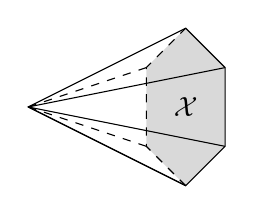
\begin{tikzpicture}[baseline=(P)]
		\coordinate (A) at (0, 1);
		\coordinate (B) at (0.5, 0.5);
		\coordinate (C) at (0.5, -0.5);
		\coordinate (D) at (0, -1);
		\coordinate (E) at (-0.5, -0.5);
		\coordinate (F) at (-0.5, 0.5);
		\coordinate (O) at (-2, 0);
		\coordinate (P) at (0, -0.1);	% For the baseline
		
		\fill[gray!50, opacity=0.6] (A) -- (B) -- (C) -- (D) -- (E) -- (F) --cycle;
		\draw (O) -- (A) -- (B) -- (C) -- (D) --cycle;
		\draw (O) -- (B);
		\draw (O) -- (C);
		\draw (O) -- (D);
		\draw[dashed] (D) -- (E) -- (F) -- (A);
		\draw[dashed] (O) -- (E);
		\draw[dashed] (O) -- (F);
		\node at (0, 0) {$\mathcal{X}$};
	\end{tikzpicture}\]
	作为一则简单练习, 请读者说明 $|X^{\lhd}| \simeq \Cone_{\mathrm{top}}(|X|) \simeq |X^{\rhd}|$. 这表明定义 \ref{def:cone-simplicial} 的锥名副其实, 左锥和右锥的差别仅在于定向.
\end{example}

通过将空间剖分为单纯形集, 可以萃取许多重要的拓扑性质, 这一进路被贴切地称为``组合拓扑学''. 进一步的讨论与实例可见 \cite[第六章]{You}.

\begin{definition}[奇异集函子]
	\index[sym1]{Sing@$\mathrm{Sing}$}
	\index{qiyiji@奇异集 (singular set)}
	对任意拓扑空间 $E$, 定义单纯形集 $\mathrm{Sing}(E)$ 使得
	\[ \mathrm{Sing}(E)_n := \Hom_{\cate{Top}}(|\Delta^n|, E), \quad n \in \Z_{\geq 0}, \]
	而 $d_i: \mathrm{Sing}(E)_n \to \mathrm{Sing}(E)_{n-1}$ (或 $s_j: \mathrm{Sing}(E)_n \to \mathrm{Sing}(E)_{n+1}$) 是沿着 $|\mathrm{d}^i|: |\Delta^{n-1}| \to |\Delta^n|$ (或 $|\mathrm{s}^j|: |\Delta^{n+1}| \to |\Delta^n|$) 的拉回, 称之为 $E$ 对应的奇异 (单纯形) 集. 这给出函子
	\[ \mathrm{Sing}: \cate{Top} \to \cate{sSet}. \]
\end{definition}

\begin{theorem}\label{prop:geom-Sing-adjunction}
	几何实现是奇异集的左伴随, 换言之, 有互逆映射
	\[\begin{tikzcd}[row sep=tiny]
		\Hom_{\cate{Top}}(|X|, E) \arrow[leftrightarrow, r, "1:1"] & \Hom_{\cate{sSet}}(X, \mathrm{Sing}(E)) \\
		\varphi \arrow[mapsto, r] & {\left[ X_n \xrightarrow{x \mapsto \varphi \circ i_{n, x}} \Hom_{\cate{Top}}(|\Delta^n|, E) \right]} \\
		\displaystyle\varinjlim_{(n, x)} \left( |\Delta^n| \xrightarrow{\psi_n(x)} E \right) & \psi = {\left[ \psi_n: X_n \to \Hom_{\cate{Top}}(|\Delta^n|, E) \right]}_{n \geq 0} , \arrow[mapsto, l]
	\end{tikzcd}\]
	其中 $X \in \Obj(\cate{sSet})$ 而 $E \in \Obj(\cate{Top})$.
\end{theorem}
\begin{proof}
	回忆到 $|X| = \varinjlim_{n, x} |\Delta^n|$. 我们有典范同构
	\begin{align*}
		\Hom_{\cate{Top}}\left( \varinjlim_{n, x} |\Delta^n| , E \right) & \rightiso \varprojlim_{n, x} \Hom_{\cate{Top}}(|\Delta^n|, E) = \varprojlim_{n, x} \mathrm{Sing}(E)_n \\
		& \rightiso \varprojlim_{n, x} \Hom_{\cate{sSet}}\left( \Delta^n, \mathrm{Sing}(E) \right) \\
		\varphi & \mapsto \left( \psi_n(x) := \varphi \circ i_{n, x} \right)_{n, x}. 
	\end{align*}
	
	任何 $\psi: X \to \mathrm{Sing}(E)$ 确定的态射族 $(\psi_n(x))_{n, x}$ 皆满足相容性, 亦即属于上式右侧的 $\varprojlim$. 若能说明指定态射 $\psi$ 相当于指定相容态射族, 证明便告完成, 然而这正是注记 \ref{rem:simplicial-density} 所确保的.
\end{proof}

\begin{remark}
	对于同伦论的研究, \S\ref{sec:closed-monoidal} 提及的 $\cate{CGHaus}$ 或许是比 $\cate{Top}$ 更方便的范畴. 由于包含函子 $\cate{CGHaus} \to \cate{Top}$ 有右伴随 $k$, 因而保 $\varinjlim$, 而 $|\Delta^n|$ 是紧生成 Hausdorff 空间, 故几何实现 (或奇异集) 中的黏合 (或取 $\Hom$) 可在 $\cate{CGHaus}$ 中操作\footnote{需要说明的是所论 $\varinjlim$ 在 $\cate{CGHaus}$ 中存在, 这步是拓扑的, 参见 \cite[III.1.8, III.2.1]{GZ67}.}. 定理 \ref{prop:geom-Sing-adjunction} 中的伴随对因之分成两段, 且以相同的符号记为
	\[\begin{tikzcd}
		\cate{sSet} \arrow[shift left, r, "{|\cdot|}"] & \cate{CGHaus} \arrow[shift left, r, "\text{包含函子}"] \arrow[shift left, l, "\mathrm{Sing}"] & \cate{Top} \arrow[shift left, l, "k"] .
	\end{tikzcd}\]
\end{remark}

对于任两个单纯形集 $X$ 和 $Y$, 它们的积定义为逐项积:
\begin{gather*}
	(X \times Y)_n = X_n \times Y_n, \\
	d_i(x, y) = (d_i(x), d_i(y)), \\
	s_j(x, y) = (s_j(x), s_j(y)).
\end{gather*}
这既是 $\cate{sSet} = \cate{Set}^{\simpDelta^{\opp}}$ 中的积, 又是在定义 \ref{def:monoidal-sObj} 中取幺半范畴 $(\cate{Set}, \times)$ 的产物. 尽管两者都是缘自范畴论的定义, 但以下的基本结果说明它们也承载几何意义.

\begin{theorem}\label{prop:realization-product}
	对于单纯形集 $X$ 和 $Y$, 我们有 $\cate{CGHaus}$ 中的典范同构
	\[ |X \times Y| \simeq |X| \times |Y|. \]
	推而广之, $\cate{CGHaus}$ 版本的 $|\cdot|$ 保有限 $\varprojlim$. 如果要求 $X$ 和 $Y$ 其中之一仅有有限多个非退化单纯形, 则 $|X \times Y| \simeq |X| \times |Y|$ 在 $\cate{Top}$ 中也成立. 
\end{theorem}

一般情形的证明颇费力, 可见 \cite[Chapter III]{GZ67} 或 \cite{Dri03}. 同构对几何实现的 $\cate{Top}$ 版本一般而言并不成立; 注意到定理对 $\cate{Top}$ 版本给出的条件并非最优.

\begin{corollary}
	记 $\cate{Grp}$ 为群范畴, 若单纯形集 $X$ 可以升级为 $\cate{sGrp}$ 的对象, 则 $|X|$ 也自然地具有拓扑群的结构; 对于其他代数结构也有类似的结果.
\end{corollary}

基于定理 \ref{prop:realization-product}, 我们有理由为 $\cate{sSet}$ 中的态射 $f, g: X \rightrightarrows Y$ 定义从 $g$ 到 $f$ 的同伦为态射 $H: X \times \Delta^1 \to X$, 使得下图交换:
\begin{equation}\label{eqn:simplicial-homotopy-prep}
	\begin{tikzcd}
		X \times \Delta^0 \arrow[d, "{\identity_X \times \mathrm{d}^0}"'] \arrow[r, "\sim"] & X \arrow[d, "f"] \\
		X \times \Delta^1 \arrow[r, "H" description] & Y \\
		X \times \Delta^0 \arrow[u, "{\identity_X \times \mathrm{d}^1}"] \arrow[r, "\sim"'] & X \arrow[u, "g"']
	\end{tikzcd}
\end{equation}

作为特例, $X \times \Delta^1 \xrightarrow{\text{投影}} X \xrightarrow{f} Y$ 的合成给出从 $f$ 到自身的常值同伦. 然而这般定义的同伦并非等价关系: 简单的例子足以说明它不满足对称性. 在同伦论中, 一般会要求 $Y$ 具有额外的性质, 比如是所谓的 Kan 复形. 此时同伦关系具有期望中的性质, 从而可以组合地开展同伦群, 弱等价等概念的研究.

尽管本书不证明定理 \ref{prop:realization-product}, 但针对 $X = \Delta^p$ 和 $Y = \Delta^q$ 的简单特例不妨多说几句. 比方说, 如何分类 $\Delta^p \times \Delta^q$ 的非退化单纯形? 问题的答案非但有助于理解积的几何实现, 相关构造也是之后需要的.

首先, 任两个偏序集 $S_1$ 和 $S_2$ 的积 $S_1 \times S_2$ 通过 $(a_1, a_2) \leq (b_1, b_2) \iff a_1 \leq b_1, \; a_2 \leq b_2$ 成为偏序集, 这也相当于将它们对应的范畴取积.

\begin{definition}\label{def:pq-shuffle}
	\index{pq-chongzu@$(p, q)$-重组 ($(p, q)$-shuffle)}
	设 $p, q \in \Z_{\geq 0}$. 所谓 \emph{$(p, q)$-重组}, 意谓一个保序单映射 $\sigma: [p+q] \to [p] \times [q]$.
\end{definition}

对任意 $n \in \Z_{\geq 0}$, 指定保序映射 $\sigma: [n] \to [p] \times [q]$ 相当于指定一对保序映射 $\sigma_-: [n] \to [p]$ 和 $\sigma_+: [n] \to [q]$; 这也相当于指定 $\Delta^p \times \Delta^q$ 的一个 $n$-单纯形. 要求 $\sigma$ 单相当于要求 $i \mapsto (\sigma_-(i), \sigma_+(i))$ 的轨迹不停顿 ($i = 0, \ldots, n$). 对于 $n = p+q$ 的情形, 状况图解为:
\begin{equation}\label{eqn:pq-shuffle-diag}
	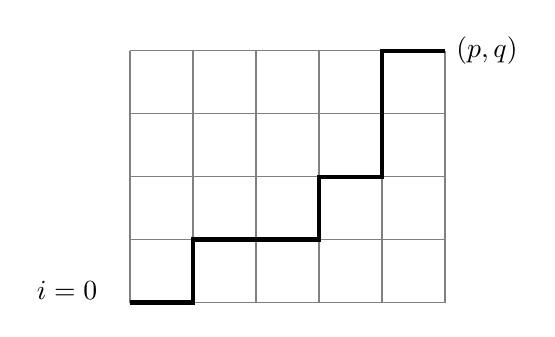
\begin{tikzpicture}[scale=0.8, baseline=(O)]
		\draw[thin, gray] (0, 0) grid (5, 4);
		\node at (-1, 0.2) {$i=0$};
		\draw[ultra thick] (0, 0) -- (1, 0) -- (1, 1) -- (2, 1) -- (3, 1) -- (3, 2) -- (4, 2) -- (4, 3) -- (4, 4) -- (5, 4) node[right] {$(p, q)$};
		\coordinate (O) at (0, 2);
	\end{tikzpicture}
	\quad
	\text{恰好移动 $p+q$ 步.}
\end{equation}
于是对于 $(p, q)$-重组 $\sigma$ 可以定义
\begin{align*}
	I_\pm & := \left\{ 1 \leq i \leq p+q : \sigma_\pm(i-1) < \sigma_\pm(i) \right\} \\
	& = \left\{ 1 \leq i \leq p+q : \sigma_\pm(i-1) = \sigma_\pm(i) - 1 \right\} \\
	& = \left\{ 1 \leq i \leq p+q: \sigma_\mp(i-1) = \sigma_\mp(i) \right\},
\end{align*}
它们满足 $I_+ \sqcup I_- = \{1, \ldots, p+q \}$. 子集 $I_+$ (或 $I_-$) 对应 \eqref{eqn:pq-shuffle-diag} 的上行 (或右行) 部分, 故 $(p, q)$-重组的另一种观点是视之为 $p$ 个符号 $\rightarrow$ 和 $q$ 个符号 $\uparrow$ 的排列, 共有 $\binom{p+q}{p}$ 种. 这些观察顺带说明 $\sigma_+$ 和 $\sigma_-$ 对于 $(p, q)$-重组是保序满射.

\begin{proposition}
	设 $p, q \in \Z_{\geq 0}$. 考虑 $\Delta^p \times \Delta^q$ 的 $n$-单纯形, 亦即保序映射 $\sigma: [n] \to [p] \times [q]$. 命 $(p_i, q_i) := \sigma(i)$, $(p', q') := (p_n - p_0, q_n - q_0)$, 则 $\sigma$ 非退化当且仅当下述条件成立:
	\begin{itemize}
		\item $p' + q' = n$;
		\item $\sigma$ 分解为 $(p', q')$-重组 $\sigma': [n] \to [p'] \times [q']$ 和形如 $f \times g$ 的保序单射 $[p'] \times [q'] \hookrightarrow [p] \times [q]$.
	\end{itemize} 
\end{proposition}
\begin{proof}
	让 $\sigma$ 对应到保序映射对 $(\sigma_-, \sigma_+)$. 按类似图 \eqref{eqn:pq-shuffle-diag} 的方式考虑 $i \mapsto (p_i, q_i)$ 的轨迹, $\sigma$ 非退化相当于说轨迹不停顿. 其余都是明白的.
\end{proof}

基于非退化单纯形的描述, 读者不妨发挥想象力来揣摩 $|\Delta^p \times \Delta^q| \simeq |\Delta^p| \times |\Delta^q|$ 在 $(p, q) = (1, 1)$ 和 $(2, 1)$ 时的道理. 例如下图是将 $|\Delta^2| \times |\Delta^1|$ 剖分为 $3$ 个四面体的结果, 对应于 $3 = \binom{3}{2}$ 个 $(2, 1)$-重组.

\begin{center}\begin{tikzpicture}[yscale=0.8]
	\coordinate (A) at (0, 0);
	\coordinate (B) at (2.2, 0.5);
	\coordinate (C) at (0.8, -0.5);
	\coordinate (P) at ($(A) + (0, -3)$);
	\coordinate (Q) at ($(B) + (0, -3)$);
	\coordinate (R) at ($(C) + (0, -3)$);

	\draw ($(A) + (-5, -0.3)$) -- ($(B) + (-5, -0.3)$) -- ($(Q) + (-5, -0.3)$) -- ($(R) + (-5, -0.3)$) -- ($(P) + (-5, -0.3)$) --cycle;
	\draw ($(A) + (-5, -0.3)$) -- ($(C) + (-5, -0.3)$) -- ($(B) + (-5, -0.3)$);
	\draw ($(C) + (-5, -0.3)$) -- ($(R) + (-5, -0.3)$);
	\draw[dashed] ($(P) + (-5, -0.3)$) -- ($(Q) + (-5, -0.3)$);
	
	\draw[-Latex] ($(B)!0.5!(Q) + (-4.5, -0.5)$) -- ($(B)!0.5!(Q) + (-3, -0.5)$);
	
	\draw (A) -- (B) -- (C) --cycle;
	\draw (A) -- (P) -- (C);
	\draw (P) -- (B);
	
	\draw[fill=white] ($(P) + (0.2, -1.2)$) -- ($(B) + (0.2, -1.2)$) -- ($(R) + (0.2, -1.2)$) --cycle;
	\draw[fill=white] ($(R) + (0.2, -1.2)$) -- ($(Q) + (0.2, -1.2)$) -- ($(B) + (0.2, -1.2)$) --cycle;
	
	\draw[fill=white] ($(P) + (0.1, -0.6)$) -- ($(R) + (0.1, -0.6)$) -- ($(C) + (0.1, -0.6)$) --cycle;
	\draw[fill=white] ($(R) + (0.1, -0.6)$) -- ($(B) + (0.1, -0.6)$) -- ($(C) + (0.1, -0.6)$) --cycle;
\end{tikzpicture}\end{center}

\begin{definition}\label{def:pq-shuffle-sgn}
	设 $\sigma$ 为 $(p, q)$-重组, 其符号定义为
	\[ \sgn(\sigma) := (-1)^{|I_\sigma|}, \quad I_\sigma := \left\{ (i, j) \in I_- \times I_+ : i > j \right\}. \]
\end{definition}

若将 $\sigma$ 视同 $p$ 个 $\rightarrow$ 和 $q$ 个 $\uparrow$ 的排列, 则 $I_\sigma$ 便是所有出现``错排'' $(\uparrow, \rightarrow)$ 的数对 $(j, i)$, 其中 $j < i$. 简单的组合学练习足以说明存在唯一的 $\tau \in \mathfrak{S}_{p+q}$ 将这般排列还原为形如 $\rightarrow \cdots \rightarrow \uparrow \cdots \uparrow$ 的样式, 而不打乱 $I_+$ 和 $I_-$ 内部的顺序, 而定义 \ref{def:pq-shuffle-sgn} 相当于说 $\sgn(\sigma) = \sgn(\tau)$.

对于 $(p, q)$-重组 $\sigma$, 调换 $\sigma_-$ 和 $\sigma_+$ 的角色给出 $(q, p)$-重组 $\sigma'$. 上述诠释和基本的组合学论证表明
\begin{equation}\label{eqn:shuffle-sign-0}
	\sgn(\sigma) = (-1)^{pq} \sgn(\sigma').
\end{equation}

准此要领, 类似地定义 $(p, q, r)$-重组为保序单射 $\sigma = (\sigma_-, \sigma_0, \sigma_+): [p+q+r] \to [p] \times [q] \times [r]$, 或理解为符号 $\rightarrow$, $\nearrow$, $\uparrow$ 的排列, 并且定义 $\sgn(\sigma)$ 为 $(-1)^{|I_\sigma|}$, 其中 $I_\sigma$ 由所有对应于 $(\rightarrow, \nearrow, \uparrow)$ 的奇排列的数组 $k > j > i$ 构成. 同样标准的组合学练习表明若 $(p, q, r)$-重组 $\sigma$ 有分解
\[ [p+q+r] \xrightarrow{\sigma_1} [p+q] \times [r] \xrightarrow{\sigma_2 \times \identity_{[r]}} [p] \times [q] \times [r], \]
则 $\sigma_1$ 是 $(p+q, r)$-重组, $\sigma_2$ 是 $(p, q)$-重组, 而且
\begin{equation}\label{eqn:shuffle-sign-1}
	\sgn(\sigma) = \sgn(\sigma_1) \sgn(\sigma_2).
\end{equation}
对于分解 $[p+q+r] \to [p] \times [q+r] \to [p] \times [q] \times [r]$ 自然也有对应的陈述.

等式 \eqref{eqn:shuffle-sign-0} 和 \eqref{eqn:shuffle-sign-1} 的本质都是组合学, 详细验证留作本章习题. 这些观察将在 \S\ref{sec:bisimplicial} 用到.

\section{Dold--Kan 对应}\label{sec:Dold-Kan}
遵循代数拓扑学的惯例, 我们将对加性范畴 $\mathcal{A}$ 考虑其上的链复形范畴 (定义 \ref{def:complex}), 记为 $\cate{Ch}(\mathcal{A})$, 连同其子范畴
\[ \cate{Ch}_{\geq 0}(\mathcal{A}) := \left\{ A = (A_n, \partial_n)_{n \in \Z} : \text{链复形}, \; \forall n < 0, \; A_n = 0 \right\}, \]
其中 $\partial_n = \partial^A_n: A_n \to A_{n-1}$. 对于 $\cate{Ch}_{\geq 0}(\mathcal{A})$ 显然只需指定资料 $(A_n)_{n \geq 0}$ 和 $(\partial_n)_{n \geq 1}$. 同理可以定义 $\cate{Ch}_{\geq m}(\mathcal{A})$; 请参照定义 \ref{def:cplx-cat-variant} 的上链复形版本.
\index[sym1]{ChA@$\cate{Ch}(\mathcal{A})$}

适当扩大所取的 Grothendieck 宇宙, 不妨假定 $\mathcal{A}$ 是加性小范畴, 见 \cite[假设 1.5.2]{Li1}. 从 $\mathcal{A}$ 可以定义单纯形对象范畴 $\cate{s}\mathcal{A}$; 对应于 $0$ 的常值单纯形对象仍记为 $0 \in \Obj(\cate{s}\mathcal{A})$. 本节旨在初步地明确这些范畴之间的关系, 更精确地说, 我们将定义三个函子
\[\begin{tikzcd}
	\cate{Ch}_{\geq 0}(\mathcal{A}) \arrow[r, "\Gamma" description] & \cate{s}\mathcal{A} \arrow[bend left, l, "{\mathrm{N}}"] \arrow[bend right, l, "{\mathrm{C}}"']
\end{tikzcd}\]
其中 $\mathrm{N}$ 仅在 $\mathcal{A}$ 为 Abel 范畴时方有定义, 而 $\mathrm{C}$ 和 $\mathrm{N}$ 都可以扩及注记 \ref{rem:semisimplicial} 所谓的半单纯形对象; 换言之, 它们不涉及退化态射.

我们的处理方式取法 \cite[\S 1.2]{LuHA}. 首务是明确相关定义.

\begin{definition}[非正规化链复形]\label{def:unnormalized-chain}
	\index{feizhengguihualianfuxing@非正规化链复形 (unnormalized chain complex)}
	\index{Moore lianfuxing@Moore 链复形 (Moore chain complex)}
	\index[sym1]{CX@$\mathrm{C}X$}
	对于 $\mathcal{A}$ 中的半单纯形对象 $X$ 和每个 $n \in \Z_{\geq 1}$, 定义
	\[ \partial_n := \sum_{i=0}^n (-1)^i d_i: X_n \to X_{n-1}; \]
	这使得 $(X_n)_{n \geq 0}$ 连同 $(\partial_n)_n$ 构成 $\cate{Ch}_{\geq 0}(\mathcal{A})$ 的对象, 称为 $X$ 给出的\emph{非正规化链复形}或 \emph{Moore 链复形}, 记为 $\mathrm{C}X$; 因此 $(\mathrm{C}X)_n = X_n$.
\end{definition}

必须说明当 $n > 1$ 时 $\partial_{n-1}\partial_n = 0$; 诚然, \eqref{eqn:simplicial-identity} 中的 $i < j \implies d_i d_j = d_{j-1} d_i$ 蕴涵
\begin{multline*}
	\partial_{n-1} \partial_n = \sum_{i=0}^{n-1} \sum_{j=0}^n (-1)^{i+j} d_i d_j \\
	= \sum_{0 \leq i < j \leq n} (-1)^{i+j} d_{j-1} d_i + \sum_{n-1 \geq i \geq j \geq 0} (-1)^{i+j} d_i d_j = 0.
\end{multline*}
此构造对 $X$ 显然是典范的, 给出函子 $\mathrm{C}$.

\begin{example}\label{eg:classifying-space-std-cplx}
	取交换环 $\Bbbk$ 和 $\mathcal{A} = \Bbbk\dcate{Mod}$. 给定群 $\Gamma$, 例 \ref{eg:classifying-space} 给出对应的单纯形集 $\mathrm{E}\Gamma$; 定义 $\Bbbk\dcate{Mod}$ 上的单纯形对象 $\Bbbk\mathrm{E}\Gamma$, 它的 $n$ 次项是以 $\mathrm{E}\Gamma$ 为基的自由 $\Bbbk$-模, $d_i$ 和 $s_i$ 则按线性延拓. 兹断言 $\mathrm{C}(\Bbbk \mathrm{E}\Gamma)$ 正是定义 \ref{def:resolution-trivial-module} 介绍的链复形 $\mathsf{L} := (\mathsf{L}_n, \partial'_n)_n$. 首先, $\mathsf{L}_n$ 按定义是以 $\Gamma^{n+1}$ 为基的自由 $\Bbbk$-模. 取从 $(\mathrm{E}\Gamma)_n = \Gamma^{n+1}$ 到 $\mathsf{L}_n$ 的映射
	\[ \left( g_1, \ldots, g_{n+1} \right) \mapsto \left(g_1 \cdots g_{n+1}, \; \ldots , \; g_n g_{n+1}, \; g_{n+1}\right). \]
	它线性地延拓到 $(\Bbbk\mathrm{E}\Gamma)_n$ 上. 请读者验证 $\sum_i (-1)^i d_i$ 依此对应到 $\partial'_n: \mathsf{L}_n \to \mathsf{L}_{n-1}$, 给出所求同构.
	
	此外, $\Gamma$ 通过 $(g_1, \ldots, g_{n+1}) \xmapsto{g} (g_1, \ldots, g_n, g_{n+1}g)$ 右作用于每个 $(\mathrm{E}\Gamma)_n$; 这反映在 $\mathsf{L}_n$ 的基上, 化作 $(g_0, \ldots, g_n) \xmapsto{g} (g_0 g, \ldots, g_n g)$; 于是我们得到定义 \ref{def:resolution-trivial-module} 赋予 $\mathsf{L}$ 的右 $\Gamma$-作用. 有鉴于此, 对链复形 $\mathrm{C}(\Bbbk\mathrm{E}\Gamma)$ 和 $\mathsf{L}$ 逐项取 $\Gamma$-余不变量的产物也相互同构, 而前者又相当于对 $\mathrm{E}\Gamma$ 逐项取商再取自由 $\Bbbk$-模. 这导致
	\[ \mathrm{C}(\Bbbk\mathrm{B}\Gamma) \simeq \mathsf{L} \dotimes{\Bbbk[\Gamma]} \Bbbk, \]
	张量积涉及增广同态 $\Bbbk[\Gamma] \to \Bbbk$; 作为推论, 群的同调 (定义 \ref{def:group-coh-ho}) 便诠释为
	\[ \Hm_n(\mathrm{B}\Gamma; \Bbbk) := \Hm_n \mathrm{C}(\Bbbk\mathrm{B}\Gamma) \simeq \Hm_n(\Gamma, \Bbbk), \quad n \in \Z_{\geq 0}. \]
	
	左式出现了单纯形集的同调, 这是定义 \ref{def:simplicial-set-homology} 即将介绍的一般构造. 本章习题将对 $\mathsf{L}$ 的正规化版本 $\overline{\mathsf{L}}$ 给出类似的同构, 它对应于定义 \ref{def:normalized-cplx} 行将讨论的正规化链复形 $\mathrm{N}(\Bbbk\mathrm{E}\Gamma)$.
\end{example}

\begin{definition}\label{def:DK-Gamma}
	取定 $\cate{Ch}_{\geq 0}(\mathcal{A})$ 的对象 $(A_n, \partial_n)_{n \geq 0}$. 按以下方式定义 $\cate{s}\mathcal{A}$ 的对象 $\Gamma(A)$.
	\[ (\Gamma A)_n := \bigoplus_{t: [n] \twoheadrightarrow [k]} A_k. \]
	
	对于 $\simpDelta$ 的任意态射 $f: [m] \to [n]$, 对应的 $f^*: (\Gamma A)_n \to (\Gamma A)_m$ 相对于上述直和分解表为以下矩阵 
	\[ \left( \Phi_{u, t} : A_k \to A_l \right)_{\substack{ u: [m] \twoheadrightarrow [l] \\ t: [n] \twoheadrightarrow [k] }}, \]
	按以下方式确定: 给定 $t: [n] \twoheadrightarrow [k]$, 作 $tf$ 的满--单分解
	\begin{equation}\label{eqn:Dold-Kan-epi-mono}\begin{tikzcd}[row sep=tiny]
		& {[n]} \arrow[twoheadrightarrow, rd, "t"] & \\
		{[m]} \arrow[ru, "f"] \arrow[twoheadrightarrow, rd, "u"'] & & {[k]} \\
		& {[l]} \arrow[hookrightarrow, ru, "v"'] &
	\end{tikzcd}\end{equation}
	\begin{itemize}
		\item 若 $l = k$, 命 $\Phi_{u, t} = \identity$;
		\item 若 $l = k-1$ 而 $v = \mathrm{d}^0$ (遗漏 $0$ 的保序单射), 命 $\Phi_{u, t} = \partial_k: A_k \to A_{k-1}$;
		\item 其余情形命 $\Phi_{u, t} = 0$.
	\end{itemize}
	留意到当 $f$ 和 $t$ 给定, 至多仅有唯一的 $u$ 使 $\Phi_{u, t} \neq 0$.
\end{definition}

关于 $\Gamma A \in \Obj(\cate{s}\mathcal{A})$ 的验证比较琐碎, 在此略过. 核心是 $(\Gamma A)_n$ 的直和项 $A_n$ 和它们在保序单映射下的行为, 其他低次直和项 $A_k$ 皆来自满态射 $[n] \twoheadrightarrow [k]$ 诱导的退化, 一般情形下 $f^*$ 的定义不过是体现此思路.

上述构造是典范的, 给出函子 $\Gamma: \cate{Ch}_{\geq 0}(\mathcal{A}) \to \cate{s}\mathcal{A}$.

\begin{definition}\label{def:normalized-cplx}
	\index{zhengguihualianfuxing@正规化链复形 (normalized chain complex)}
	\index[sym1]{NX@$\mathrm{N}X$}
	设 $\mathcal{A}$ 是 Abel 范畴. 对 $\mathcal{A}$ 中的半单纯形对象 $X$ 和所有 $n \in \Z_{\geq 0}$ 和 $0 \leq k \leq n$ 定义
	\begin{align*}
		(\mathrm{N} X)_n & := \bigcap_{i=1}^n \Ker\left[ d_i: X_n \to X_{n-1} \right], \quad n \geq 1, \\
		(\mathrm{N} X)_0 & := X_0.
	\end{align*}

	连同 $X_n \xrightarrow{d_0} X_{n-1}$ 所诱导的态射族 $\mathrm{N}X_n \to \mathrm{N}X_{n-1}$ (请用 \eqref{eqn:simplicial-identity} 验证), 合理地记为 $\partial_n$, 它们构成 $\cate{Ch}_{\geq 0}(\mathcal{A})$ 的对象 $\mathrm{N}X$, 称为 $X$ 对应的\emph{正规化链复形}.
\end{definition}

\begin{proposition}\label{prop:Dold-Kan-u}
	对如上之 $X$ 和每个 $n \geq 0$, 记 $u_n: (\mathrm{N}X)_n \hookrightarrow X_n$ 为自然嵌入, 则 $(u_n)_{n \geq 0}$ 构成 $\cate{Ch}_{\geq 0}(\mathcal{A})$ 中的单态射 $u: \mathrm{N}X \to \mathrm{C}X$, 它对 $X$ 满足函子性.
\end{proposition}
\begin{proof}
	直接来自 $\mathrm{N}X$ 和 $\mathrm{C}X$ 的定义.
\end{proof}

后续几则结果是 Dold--Kan 定理 \ref{prop:Dold-Kan} 的必要铺垫.

\begin{lemma}\label{prop:DK-N-unit}
	设 $\mathcal{A}$ 是 Abel 范畴, 则对所有 $A \in \Obj(\cate{Ch}_{\geq 0}(\mathcal{A}))$ 和 $n \geq 0$ 皆有 $\mathrm{N}\Gamma(A)_n = A_n$. 这给出函子的同构 $\eta: \identity_{\cate{Ch}_{\geq 0}(\mathcal{A})} \rightiso \mathrm{N}\Gamma$.
\end{lemma}
\begin{proof}
	给定 $t: [n] \twoheadrightarrow [k]$, 注意到当 $k < n$ 时, 总可以取 $1 \leq i \leq n$ 使得 $t^{-1}(t(i))$ 至少有两个元素, 从而 $t \mathrm{d}^i$ 满, 使下图交换:
	\[\begin{tikzcd}[row sep=tiny]
		& {[n]} \arrow[twoheadrightarrow, rd, "t"] & \\
		{[n-1]} \arrow[ru, "{\mathrm{d}^i}"] \arrow[twoheadrightarrow, rd, "{t\mathrm{d}^i}"'] & & {[k]} \\
		& {[k]} \arrow[ru, "{\identity}"'] &
	\end{tikzcd}\]
	代入定义 \ref{def:DK-Gamma} 遂知 $\mathrm{N}\Gamma(A)_n$ 包含于 $\identity: [n] \to [n]$ 对应的直和项 $A_n$. 然而易证该定义进一步蕴涵 $\mathrm{N}\Gamma(A)_n = A_n$, 而且 $\mathrm{N}\Gamma(A)_{n+1} \to \mathrm{N}\Gamma(A)_n$ 正是 $\partial_{n+1}: A_{n+1} \to A_n$. 证毕.
\end{proof}

\begin{lemma}\label{prop:GammaN-adjunction}
	设 $\mathcal{A}$ 是 Abel 范畴, 则先前定义的函子给出伴随对
	\[\begin{tikzcd}
		\Gamma: \cate{Ch}_{\geq 0}(\mathcal{A}) \arrow[shift left, r] & \cate{s}\mathcal{A} : \mathrm{N} \arrow[shift left, l]
	\end{tikzcd}\]
	\begin{itemize}
		\item 对应的单位态射是引理 \ref{prop:DK-N-unit} 的同构 $\eta$;
		\item 余单位态射 $\epsilon: \Gamma \mathrm{N}\to \identity_{\cate{s}\mathcal{A}}$ 描述如下: 给定 $t: [n] \twoheadrightarrow [k]$, 在 $\Gamma\mathrm{N}(X)_n$ 中相应的直和项 $(\mathrm{N}X)_k$ 上, $\epsilon_{X, n}$ 是 $(\mathrm{N}X)_k \subset X_k \xrightarrow{t^*} X_n$.
	\end{itemize}
\end{lemma}
\begin{proof}
	给定 $A \in \Obj(\cate{Ch}_{\geq 0}(\mathcal{A}))$ 和 $X \in \Obj(\cate{s}\mathcal{A})$, 首要目标是证
	\[ \Hom_{\cate{s}\mathcal{A}}(\Gamma(A), X) \xrightarrow{\mathrm{N}} \Hom_{\cate{Ch}_{\geq 0}(\mathcal{A})}(\mathrm{N}\Gamma(A), \mathrm{N}(X)) \xrightarrow{\eta_A^*} \Hom_{\cate{Ch}_{\geq 0}(\mathcal{A})}(A, \mathrm{N}(X)) \]
	的合成为双射. 其逆具体定义如下. 给定 $\phi = (\phi_n)_{n \geq 0}: A \to \mathrm{N}(X)$, 定义态射
	\[ \Phi_n: (\Gamma A)_n = \bigoplus_{t: [n] \twoheadrightarrow [k]} A_k \to X_n \]
	使得它在对应 $t: [n] \twoheadrightarrow [k]$ 的直和项上是
	\[ A_k \xrightarrow{\phi_k} (\mathrm{N}X)_k \subset X_k \xrightarrow{t^*} X_n \]
	的合成. 对于如上之 $t$ 和任意的 $f: [m] \to [n]$, 作 $tf$ 的满--单分解如 \eqref{eqn:Dold-Kan-epi-mono}, 并考虑 $\mathcal{A}$ 中的图表 (参见定义 \ref{def:DK-Gamma}):
	\[\begin{tikzcd}[column sep=large]
		A_k \arrow[r, "\phi_k"] \arrow[d, "{\Phi_{u, t}}"'] & (\mathrm{N}X)_k \arrow[hookrightarrow, r] \arrow[d, "{v^*|_{(\mathrm{N}X)_k}}"] & X_k \arrow[r, "{t^*}"] \arrow[d, "{v^*}"] & X_n \arrow[d, "{f^*}"] \\
		A_l \arrow[r, "\phi_l"'] & (\mathrm{N}X)_l \arrow[hookrightarrow, r] & X_l \arrow[r, "{u^*}"'] & X_m
	\end{tikzcd}\]
	左侧方块因正规化链复形 $\mathrm{N}X$ 的定义而交换, 中间方块显然交换, 右侧方块因 $tf = vu$ 交换. 因此 $\Phi = (\Phi_n)_n$ 是 $\cate{s}\mathcal{A}$ 的态射.
	
	关于 $\eta_A^* \mathrm{N}$ 和 $\phi \mapsto \Phi$ 互逆的验证不过是例行公事. 在 $\phi \mapsto \Phi$ 的描述中取 $\phi = \identity_{\mathrm{N}X}$, 结果正是断言中的 $\epsilon$.
\end{proof}

\begin{lemma}\label{prop:DK-Ab}
	取 $\mathcal{A} = \cate{Ab}$, 则 $\Gamma$ 是等价; 精确地说, 伴随对
	$\begin{tikzcd}
		\Gamma: \cate{Ch}_{\geq 0}(\cate{Ab}) \arrow[shift left, r] & \cate{s}\cate{Ab} : \mathrm{N} \arrow[shift left, l]
	\end{tikzcd}$
	是 \cite[定理 2.6.12]{Li1} 所谓的伴随等价.
\end{lemma}
\begin{proof}
	要点在于验证引理 \ref{prop:GammaN-adjunction} 描述的余单位态射 $\epsilon$ 为同构. 选定 $X \in \Obj(\cate{s}\mathcal{A})$, 兹断言 $\epsilon_{X, n}: \Gamma (\mathrm{N}X)_n \to X_n$ 对每个 $n \geq 0$ 皆单. 设 $x = (x_t)_t$ 属于左式, 其中 $t$ 遍历保序满射 $[n] \twoheadrightarrow [k]$. 给定 $t$, 定义保序单射
	\begin{align*}
		s = s_t : [k] & \hookrightarrow [n] \\
		i & \mapsto \min t^{-1}(i) ,
	\end{align*}
	它满足 $ts = \identity_{[k]}$. 现在假定 $x \neq 0$, 记
	\[ S := \left\{t: x_t \neq 0 \right\} \neq \emptyset. \]
	取最小的 $k$ 使得存在属于 $S$ 的 $t: [m] \twoheadrightarrow [k]$, 再取如此之 $t$ 使 $\sum_{i=0}^k \min t^{-1}(i)$ 尽量小, 并构造 $s$. 今将往证 $s^*(\epsilon_{X, n}(x)) = x_t \in X_k$, 以此说明 $\epsilon_{X, n}(x) \neq 0$.
	
	基于 $\epsilon_{X, n}$ 的具体描述, 仅须对 $t': [n] \twoheadrightarrow [k']$ 证明 $s^* (t')^*(x_{t'}) \neq 0$ 蕴涵 $t = t'$ 即可. 命 $u := t's: [k] \to [k']$. 当 $t' \notin S$ 时 $x_{t'} = 0$, 故以下设 $t' \in S$ 满足 $s^* (t')^*(x_{t'}) = u^* (x_{t'}) \neq 0$.
	
	由于 $t$ 保序而且满, $\min t^{-1}(0) = 0$, 对 $t'$ 亦然, 故 $u(0) = 0$. 又由 $x_{t'} \in (\mathrm{N}X)_{k'}$ 可推知仅当 $\Image(u) \supset \{1, \ldots, k'\}$ 时才可能有 $u^* (x_{t'}) \neq 0$. 故以下可设 $u$ 满, $k$ 的取法遂蕴涵 $k' = k$ 而 $u = \identity$.
	
	综之, $t'\left( \min t^{-1}(i) \right) = i$ 对 $i = 0, \ldots, k$ 皆成立, 故 $\min (t')^{-1}(i) \leq \min t^{-1}(i)$. 回顾 $t$ 的取法可得 $\min (t')^{-1}(i) = \min t^{-1}(i)$ 对所有 $0 \leq i \leq k$ 成立; 稍加思索, 可知这相当于说 $t = t'$. 至此证得 $\epsilon_{X, n}$ 单.
	
	以下对 $n$ 递归地证明 $\epsilon_{X, n}$ 满. 兹断言对所有 $0 \leq i \leq n$ 皆有
	\[ \Image\left( \epsilon_{X, n} \right) \supset X(i)_n := \bigcap_{i < j \leq n} \Ker(d_j) \subset X_n. \]
	
	当 $i = 0$ 时 $X(i)_n = (\mathrm{N}X)_n$, 上式容易从 $\epsilon_{X, n}$ 的具体描述导出, 而我们的目标是 $i=n$. 设 $n \geq i \geq 1$ 而 $y \in X(i)_n$. 关于 $n-1$ 的递归假设和 $\epsilon_{X, n}$ 的描述蕴涵
	\[ s_{i-1} d_i(y) \in s_{i-1}\left( \Image\left(\epsilon_{X, n-1}\right) \right) \subset \Image\left( \epsilon_{X, n} \right). \]

	另一方面, 单纯形等式 \eqref{eqn:simplicial-identity} 蕴涵
	\begin{gather*}
		d_i s_{i-1} d_i = d_i, \\
		j > i \implies d_j s_{i-1} d_i = s_{i-1} d_{j-1} d_i = s_{i-1}  d_i d_j.
	\end{gather*}
	故 $y - s_{i-1} d_i(y) \in X(i-1)_n$, 而关于 $i-1$ 的递归假设说明它属于 $\Image\left( \epsilon_{X, n} \right)$. 综之 $y \in \Image\left( \epsilon_{X, n} \right)$, 明所欲证.
\end{proof}

\begin{theorem}[A.\ Dold, D.\ Kan]\label{prop:Dold-Kan}
	\index{Dold-Kan duiying@Dold--Kan 对应 (Dold--Kan correspondence)}
	对于任意加性范畴 $\mathcal{A}$, 函子 $\Gamma: \cate{Ch}_{\geq 0}(\mathcal{A}) \to \cate{s}\mathcal{A}$ 是全忠实的.
	\begin{itemize}
		\item 若 $\mathcal{A}$ 还是 \S\ref{sec:direct-sum} 提及的 Karoubi 范畴, 亦即所有幂等元都有核, 则 $\Gamma$ 是范畴等价.
		\item 若进一步要求 $\mathcal{A}$ 是 Abel 范畴 (因而也是 Karoubi 范畴), 则 $\mathrm{N}$ 是 $\Gamma$ 的拟逆函子,
		$\begin{tikzcd}
			\Gamma: \cate{Ch}_{\geq 0}(\mathcal{A}) \arrow[shift left, r] & \cate{s}\mathcal{A} : \mathrm{N} \arrow[shift left, l]
		\end{tikzcd}$
		是伴随等价, 伴随对的单位和余单位态射由引理 \ref{prop:GammaN-adjunction} 描述.
	\end{itemize}
\end{theorem}
\begin{proof}
	考虑函子
	\[ \tilde{h}_{\mathcal{A}}: \mathcal{A} \to \tilde{\mathcal{A}}^\wedge := \cate{Ab}^{(\mathcal{A}^{\opp})}, \quad Y \mapsto \Hom_{\mathcal{A}}(\cdot, Y). \]
	它和忘却函子 $\cate{Ab} \to \cate{Set}$ 合成等于 \S\ref{sec:Yoneda} 回顾的米田嵌入 $h_{\mathcal{A}}: \mathcal{A} \to \mathcal{A}^\wedge$. 函子 $\tilde{h}_{\mathcal{A}}$ 是全忠实的, 这点不过是 $\cate{Ab}$-充实版本的米田引理, 但也可以从原版推导: 对任意 $Y_1, Y_2 \in \Obj(\mathcal{A})$, 合成映射
	\[ \Hom_{\mathcal{A}}(Y_1, Y_2) \to \Hom_{\tilde{\mathcal{A}}^\wedge}\left(\tilde{h}_{\mathcal{A}}(Y_1), \tilde{h}_{\mathcal{A}}(Y_2) \right) \to \Hom_{\mathcal{A}^\wedge}\left( h_{\mathcal{A}}(Y_1), h_{\mathcal{A}}(Y_2)\right) \]
	已知是双射, 但第二段明显是单射, 由此可知两段皆为双射.
	
	命题 \ref{prop:functor-cat-Abel} 表明 $\tilde{\mathcal{A}}^\wedge$ 自然地成为 Abel 范畴. 以相同的符号标记 $\tilde{h}_{\mathcal{A}}$ 在链复形和单纯形对象上诱导的函子, 考虑图表:
	\begin{equation*}\begin{tikzcd}
		\cate{Ch}_{\geq 0}(\mathcal{A}) \arrow[d, "{\tilde{h}_{\mathcal{A}}}"'] \arrow[r, "\Gamma"] & \cate{s}\mathcal{A} \arrow[d, "{\tilde{h}_{\mathcal{A}}}"] \\
		\cate{Ch}_{\geq 0}(\tilde{\mathcal{A}}^\wedge) \arrow[r, "\Gamma"'] & \cate{s}\tilde{\mathcal{A}}^\wedge
	\end{tikzcd}\end{equation*}
	此图精确到典范同构是交换的. 上一段的观察说明两个垂直箭头全忠实, 而逐对象地应用关于 $\cate{Ab}$ 的引理 \ref{prop:DK-Ab}, 可见第二行是范畴等价. 于是第一行的 $\Gamma$ 全忠实.
	
	对于任意函子 $F: \mathcal{C} \to \mathcal{C}'$, 我们称 $X' \in \Obj(\mathcal{C}')$ 属于 $F$ 的本质像, 如果存在 $X \in \cate{Obj}(\mathcal{C})$ 使得 $X' \simeq FX$. 搭配引理 \ref{prop:DK-Ab} 对 $\cate{Ch}_{\geq 0}(\cate{Ab}) \to \cate{s}\cate{Ab}$ 的拟逆的描述, 便能得到以下结论: $X \in \Obj(\cate{s}\mathcal{A})$ 属于 $\Gamma$ 的本质像当且仅当 $\mathrm{N} \tilde{h}_{\mathcal{A}}(X)_n$ 对每个 $n \geq 0$ 皆属于 $\tilde{h}_{\mathcal{A}}: \mathcal{A} \to \tilde{\mathcal{A}}^\wedge$ 的本质像.
	
	注意到 $\tilde{h}_{\mathcal{A}}: \mathcal{A} \to \tilde{\mathcal{A}}^\wedge$ 保有限直和.
	当 $\mathcal{A}$ 是 Karoubi 范畴时, $\mathcal{A} \to \tilde{\mathcal{A}}^\wedge$ 的本质像因而对萃取直和项保持封闭; 既然 $\mathrm{N} \tilde{h}_{\mathcal{A}}(X)_n$ 是 $\Gamma\mathrm{N} \tilde{h}_{\mathcal{A}}(X)_n \simeq h_{\mathcal{A}}(X)_n$ 的直和项, 此时 $\Gamma$ 全忠实本质满, 从而是等价.
	
	最后, 伴随等价定理 \cite[定理 2.6.12]{Li1} 确保 $\Gamma: \cate{Ch}_{\geq 0}(\mathcal{A}) \to \cate{s}\mathcal{A}$ 的拟逆总能扩充为其右伴随. 当 $\mathcal{A}$ 是 Abel 范畴时, 引理 \ref{prop:GammaN-adjunction} 已经说明 $\mathrm{N}$ 是 $\Gamma$ 的右伴随, 因而是 $\Gamma$ 的拟逆. 明所欲证.
\end{proof}

\begin{convention}
	基于此, 当 $\mathcal{A}$ 是 Karoubi 范畴时, 可以选定 $\Gamma: \cate{Ch}_{\geq 0}(\mathcal{A}) \to \cate{s}\mathcal{A}$ 的拟逆函子, 并且合理地记之为 $\mathrm{N}$.
\end{convention}

虽然 $\mathrm{N}X$ 的初始定义是 $\mathrm{C}X$ 的子对象, 但是它也可以理解为商, 后者在很多场合更加方便. 以下便来说明这一点.

考虑 Karoubi 范畴 $\mathcal{A}$ 和 $X \in \Obj(\cate{s}\mathcal{A})$. 对所有 $n \geq 0$ 定义 $\mathcal{A}$ 中的态射 $\Psi_n$, 其刻画是使下图对所有 $0 \leq j < n$ 交换:
\[\begin{tikzcd}
	\bigoplus_{0 \leq i < n} X_{n-1} \arrow[r, "\Psi_n"] & X_n \\
	X_j \arrow[hookrightarrow, u, "\text{直和项}"] \arrow[ru, "{s_j}"'] &
\end{tikzcd}\]
因此考虑 $\Coker(\Psi_n)$ (亦即 $\Psi_n$ 和 $0$ 的余等化子) 相当于从 $X_n$ 抹去所有退化部分, 至少当 $\mathcal{A}$ 是 Abel 范畴时可作此观; 次一结果说明 $\Coker(\Psi_n)$ 不只存在, 还通过命题 \ref{prop:Dold-Kan-u} 的自然嵌入 $u: \mathrm{N}X \to \mathrm{C}X$ 等同于 $(\mathrm{N}X)_n$, 这就提供了看待 $\mathrm{N}X$ 的另一视角.

\begin{proposition}\label{prop:Dold-Kan-v}
	在上述情境中, $\Coker(\Psi_n)$ 存在并且典范同构于 $(\mathrm{N}X)_n$. 考虑相应的合成 $v_n: X_n \twoheadrightarrow \Coker(\Psi_n) \rightiso (\mathrm{N}X)_n$, 则 $(v_n)_n$ 给出态射 $v: \mathrm{C}X \to \mathrm{N}X$, 它对 $X$ 有函子性, 并且对自然嵌入 $u: \mathrm{N}X \hookrightarrow \mathrm{C}X$ 满足 $vu = \identity_{\mathrm{N}X}$.
\end{proposition}
\begin{proof}
	鉴于定理 \ref{prop:Dold-Kan}, 不妨假设 $X = \Gamma A$, 其中 $A \in \Obj(\cate{Ch}_{\geq 0}(\mathcal{A}))$. 于是 $\Psi_n$ 表作
	\[ \bigoplus_{0 \leq i < n} \bigoplus_{t: [n-1] \twoheadrightarrow [k]} A_k \to \bigoplus_{t': [n] \twoheadrightarrow [k] } A_k. \]
	回忆函子 $\Gamma$ 的定义 \ref{def:DK-Gamma} 可见 $\Psi_n$ 在左式的 $(i, t)$-直和项按下述方式作用: 取 $[n] \xrightarrow{\mathrm{s}^i} [n-1] \xrightarrow{t} [k]$ 的合成, 这仍是保序满射, 记为 $t'$, 而 $A_k$ 恒等地映至右式的 $t'$-直和项 $A_k$.
	
	观察到 $t': [n] \twoheadrightarrow [k]$ 来自这样的 $(i, t)$ 当且仅当 $k < n$. 以引理 \ref{prop:DK-N-unit} 的 $\eta$ 定义 $v_n$ 为合成 $(\Gamma A)_n \xrightarrow{\text{投影}} A_n \xrightarrow[\sim]{\eta} (\mathrm{N}\Gamma A)_n$. 综上可见
	\[ [\text{商}: (\Gamma A)_n \to \Coker \Psi_n] \simeq [v_n: (\Gamma A)_n \twoheadrightarrow (\mathrm{N}\Gamma A)_n ] . \]
	
	展开定义可见 $v_n u_n = \identity_{(\mathrm{N}\Gamma A)_n}$ 几近同义反复. 接着来说明 $(v_n)_n$ 给出 $\cate{Ch}_{\geq 0}(\mathcal{A})$ 中的态射 $v$, 这相当于说下图外框交换
	\[\begin{tikzcd}[column sep=large]
		(\Gamma A)_n \arrow[r, "{\sum_i (-1)^i d^{\Gamma A}_i}"] \arrow[d, "\text{投影}"'] & (\Gamma A)_{n-1} \arrow[d, "\text{投影}"] \\
		A_n \arrow[r, "{\partial^A_n}"] \arrow[d, "\eta"'] & A_{n-1} \arrow[d, "\eta"] \\
		(\mathrm{N}\Gamma A)_n \arrow[r, "{\partial^{\mathrm{N}\Gamma A}_n}"'] & (\mathrm{N}\Gamma A)_{n-1}
	\end{tikzcd}\]
	下半部交换是因为 $\eta$ 是态射, 上半部交换则是 $d^{\Gamma A}_i$ 定义的直接操练 (在定义 \ref{def:DK-Gamma} 中取 $f = \mathrm{d}^i$). 最后, $v$ 显然对 $X$ 有函子性.
\end{proof}

下一个目标是对 Abel 范畴的情形更精密地比较 $\mathrm{C}$ 和 $\mathrm{N}$. 对于链复形之间的态射有同伦的概念, 见定义 \ref{def:homotopy} 和注记 \ref{rem:Hom-chain-cplx}. 链复形之间的态射若在同调层次诱导同构, 则称为拟同构.

\begin{theorem}\label{prop:Dold-Kan-N-C}
	设 $\mathcal{A}$ 为 Abel 范畴, $X \in \Obj(\cate{s}\mathcal{A})$, 则引理 \ref{prop:Dold-Kan-u} 的 $u: \mathrm{N}X \to \mathrm{C}X$ 和命题 \ref{prop:Dold-Kan-v} 的 $v: \mathrm{C}X \to \mathrm{N}X$ 皆是拟同构.
\end{theorem}
\begin{proof}
	已知 $vu = \identity_{\mathrm{N}X}$, 证 $v$ 是拟同构即可. 由于 $v$ 有右逆, 因而满, 链复形的长正合列 (命题 \ref{prop:long-exact-sequence-ses}) 将问题化为证 $\Ker(v)$ 零调. 鉴于定理 \ref{prop:Dold-Kan}, 以下不妨设 $X = \Gamma A$, 其中 $A \in \Obj(\cate{Ch}_{\geq 0}(\mathcal{A}))$. 因此
	\begin{gather*}
		(\mathrm{C}X)_n = \bigoplus_{t: [n] \twoheadrightarrow [k]} A_k, \\
		\partial_n : (\mathrm{C}X)_n \to (\mathrm{C}X)_{n-1}.
	\end{gather*}
	
	给定 $n \geq 0$ 和 $i \in \Z$, 记 $(\mathrm{C}^{\leq i} X)_n$ 为 $(\mathrm{C}X)_n$ 中由满足
	\[ \exists \; j, \quad \max\{n-i, 1\} \leq j \leq n, \quad t(j) = t(j-1) \]
	的直和项截出的子对象. 我们有 $i \leq i' \implies (\mathrm{C}^{\leq i} X)_n \subset (\mathrm{C}^{\leq i'} X)_n$.

	因为 $v_n$ 不外是向 $t = \identity_{[n]}$ 的直和项作投影, 当 $i \geq n-1$ 时 $(\mathrm{C}^{\leq i} X)_n = \Ker(v_n)$. 以下来说明
	\begin{equation}\label{eqn:Dold-Kan-N-C-aux0}
		\left( (\mathrm{C}^{\leq i} X)_n \right)_{n \geq 0} \;\text{给出}\; \mathrm{C}X \;\text{的子链复形}\; \mathrm{C}^{\leq i} X.
	\end{equation}

	为了证明这点, 选定满足前述条件的 $t: [n] \twoheadrightarrow [k]$ 和 $\max\{n-i, 1\} \leq j \leq n$. 今后记 $d_i = d_i^X$, $s_j = s_j^X$. 对任意 $0 \leq h \leq n$, 在图表 \eqref{eqn:Dold-Kan-epi-mono} 中取 $m = n-1$ 和 $f = \mathrm{d}^h : [n-1] \hookrightarrow [n]$.
	\begin{itemize}
		\item 设 $h \notin \{j-1, j\}$, 命 $j' := (\mathrm{d}^h)^{-1}(j)$, 则 $u: [n-1] \twoheadrightarrow [l]$ 满足 $u(j') = u(j'-1)$, 而且易见 $n - 1 - i \leq j' \leq n-1$. 此时 $(-1)^h d_h: X_n \to X_{n-1}$ 将 $A_k$ 映到 $u$ 在 $(\mathrm{C}^{\leq i} X)_{n-1}$ 中确定的直和项.
		\item 承上, 若进一步要求 $h \geq n-i-1$, 则 $j'$ 的范围还可以细化为 $n-i \leq j' \leq n-1$; 换言之, 此时 $A_k$ 的像落在 $(\mathrm{C}^{\leq i-1} X)_{n-1}$.
		\item 对于 $h \in \{j-1, j\}$ 的情形, 请读者验证 $t\mathrm{d}^{j-1} = t\mathrm{d}^j$; 由此可得 $d_{j-1}, d_j: X_n \rightrightarrows X_{n-1}$ 在 $t$ 对应的直和项 $A_k$ 上相同, $(-1)^{j-1} d_{j-1}$ 和 $(-1)^j d_j$ 在此相消.
	\end{itemize}
	这就确立了 \eqref{eqn:Dold-Kan-N-C-aux0}; 第二和第三点还顺带给出同余式
	\begin{equation}\label{eqn:Dold-Kan-N-C-aux}
		\sum_{h=0}^n (-1)^h d_h \equiv \sum_{h=0}^{n-i-2} (-1)^h d_h \pmod{ \mathrm{C}^{\leq i-1} X }.
	\end{equation}

	综上, 问题化约为证 $\mathrm{C}^{\leq i} X$ 零调. 命
	\[ D := \mathrm{C}^{\leq i} X / \mathrm{C}^{\leq i-1} X. \]
	留意到 $\mathrm{C}^{< -1} X = 0$. 链复形的长正合列遂将问题归结为递归地证明 $D$ 零调 ($i \geq 0$).
	
	为了证明 $D$ 零调. 考虑态射族
	\begin{gather*}
		(-1)^{n-i-1} s_{n-i-1}: X_n \to X_{n+1}, \quad n \geq i+1.
	\end{gather*}
	简单的验证说明它们保持 $(\mathrm{C}^{\leq i-1} X)_\bullet$ 和 $(\mathrm{C}^{\leq i} X)_\bullet$ (这是最优选取), 从而诱导
	\[ h_n: D_n \to D_{n+1}. \]
	
	我们将 $s_k$ 的定义按零延拓到所有 $k \in \Z$, 借此将 $h_n$ 的定义按零延拓到 $n \leq i$ 的情形; 观察到 $n \leq i \implies D_n = 0$, 因此这是唯一合理的选择. 兹断言
	\[ \partial^D_{n+1} h_n + h_{n-1} \partial^D_n = \identity_{D_n}, \quad n \in \Z. \]
	这将说明 $D$ 零调. 首先是应用 \eqref{eqn:Dold-Kan-N-C-aux} 得到
	\[ \partial^D_n = \sum_{j=0}^{n-i-2} (-1)^j d_j \;\bmod\; \mathrm{C}^{\leq i-1}(X)_{n-1}. \]
	搭配 \eqref{eqn:simplicial-identity} 可见当 $n \geq i+1$ 时
	\begin{align*}
		\partial^D_{n+1} h_n & = (-1)^{n-i-1} \sum_{j=0}^{n-i-1} (-1)^j d_j s_{n-i-1} \; \bmod\; \mathrm{C}^{\leq i-1}(X)_n \\
		& = (-1)^{n-i-1} \sum_{j=0}^{n-i-2} (-1)^j s_{n-i-2} d_j + \identity_{\mathrm{C}^{\leq i}(X)_n} \;\bmod\; \mathrm{C}^{\leq i-1}(X)_n \\
		& = -h_{n-1} \partial^D_n + \identity_{D_n}.
	\end{align*}
	等式在 $n \leq i$ 时也平凡地成立. 断言得证.
\end{proof}

\begin{remark}
	理所当然, 我们也希望对复形范畴 $\cate{C}(\mathcal{A})$ 或者其子范畴 $\cate{C}_{\leq 0}(\mathcal{A})$, $\cate{C}_{\geq 0}(\mathcal{A})$ 获取本节各种定理的相应版本, 特别是 Dold--Kan 对应. 对此至少有两种简单进路: 一是镜射, 二是倒转或对偶.
	\begin{enumerate}
		\item 如注记 \ref{rem:cochain-vs-chain} 所述, $\cate{C}(\mathcal{A})$ 和 $\cate{Ch}(\mathcal{A})$ 通过 $X^n = X_{-n}$ 和 $d^n = \partial_{-n}$ 彼此对应. 本节的所有结果都能借此搬运到复形上, 例如定理 \ref{prop:Dold-Kan} 的镜射版本是 $\cate{C}_{\leq 0}(\mathcal{A})$ 和 $\cate{s}\mathcal{A}$ 之间的伴随等价.
		\item 另一种方法是考虑余单纯形范畴 $\cate{cs}\mathcal{A}$. 我们有范畴等价
		\[ \cate{cs}\mathcal{A} \simeq \cate{s}\left(\mathcal{A}^{\opp}\right)^{\opp} \simeq \cate{Ch}_{\geq 0}(\mathcal{A}^{\opp})^{\opp} \simeq \cate{C}_{\geq 0}(\mathcal{A}), \]
		最后一步是反转箭头的产物, 如注记 \ref{rem:cochain-vs-chain}.
	\end{enumerate}
	关于正规化复形等操作也都能类似地翻译到复形范畴中.
\end{remark}

\section{同调计算}\label{sec:homology-computation}
函子 $\mathrm{C}$ 或 $\mathrm{N}$ 的经典应用是定义单纯形集的同调, 这与代数拓扑学的研究息息相关.

\begin{definition}\label{def:free-simplicial-Ab}
	对任意 $K \in \Obj(\cate{sSet})$, 定义 $\Z K \in \Obj(\cate{sAb})$ 使得 $(\Z K)_n$ 是以 $K_n$ 为基的自由 $\Z$-模, 而其上的 $d_i, s_j$ 来自 $K$ 带有的映射. 这给出函子 $\Z(\cdot): \cate{sSet} \to \cate{sAb}$.
\end{definition}

\begin{proposition}\label{prop:free-simplicial-Ab-adjunction}
	我们有自然的伴随对
	$\begin{tikzcd}
		\Z(\cdot): \cate{sSet} \arrow[shift left, r] & \cate{sAb}: \text{忘却} \arrow[shift left, l]
	\end{tikzcd}$.
\end{proposition}
\begin{proof}
	函子 $\Z(\cdot)$ 和忘却都是逐次地定义的. 一切化为自由--忘却伴随对 $\cate{Set} \leftrightarrows \cate{Ab}$.
\end{proof}

对于所有 $X \in \Obj(\cate{sAb})$, 指定态射 $\Z\Delta^n \to X$ 因而便相当于指定 $X_n$ 的元素.

此外, $\Z(X \times Y) \simeq \Z X \otimes \Z Y$, 右式的 $\otimes$ 代表逐次地取 $X_n \dotimes{\Z} Y_n$.

\begin{definition}\label{def:simplicial-set-homology}
	\index[sym1]{Hn}
	\index[sym1]{Hnn}
	对于单纯形集 $K$ 和任意 $n \in \Z_{\geq 0}$, 记 $\Hm_n(K; \Z) := \Hm_n\left(\mathrm{C}(\Z K) \right)$, 称为 $K$ 的 $n$ 次同调群; 这给出一族函子 $\Hm_n(\cdot; \Z): \cate{sSet} \to \cate{Ab}$.
	\begin{itemize}
		\item 推而广之, 可以定义系数为 $\Z$-模 $M$ 的同调 $\Hm_n(K; M) := \Hm_n\left(\mathrm{C}(\Z K) \otimes M \right)$, 其中 $\cdot \otimes M$ 代表将链复形逐项地取 $\cdot \dotimes{\Z} M$ 的产物.
	
		\item 系数为 $M$ 的上同调定义为 $\Hm^n(K; M) := \Hm^n\left( \Hom_{\Z}(\mathrm{C}(\Z K), M) \right)$, 括号内视作复形. 根据 $\Z(\cdot)$ 的泛性质, 复形的 $n$ 次项也可以等同于
		\[ \mathrm{Maps}(K_n, M) := \left\{ \text{映射}\; K_n \to M \right\}, \]
		它按照逐点运算成为 $\Z$-模, 微分同态则等同于 $\sum_i (-1)^i (d_i)^*$.
	\end{itemize}
\end{definition}

若在上述定义中以 $\mathrm{N}(\Z K)$ 代 $\mathrm{C}(\Z K)$, 得到的同调群 (或上同调) 群是典范同构的, 这是定理 \ref{prop:Dold-Kan-N-C} 的推论. 采用 $\mathrm{N}(\Z K)$ 有时更为简单, 这是因为命题 \ref{prop:Dold-Kan-v} 导致
\[ \mathrm{N}(\Z K)_n = \bigoplus_{x \in K^{\mathrm{nd}}_n} \Z x, \]
此处 $K^{\mathrm{nd}}_n \subset K_n$ 代表非退化单纯形所成子集, 而 $\mathrm{N}(\Z K)_n \to \mathrm{N}(\Z K)_{n-1}$ 是先取 $\sum_{i=0}^n (-1)^i d_i$ 再向 $K^{\mathrm{nd}}_{n-1}$ 部分作投影. 例如
\begin{align*}
	\mathrm{N}(\Z \Delta^0) & = \Z\; \text{置于 $0$ 次项}, \\
	\mathrm{C}(\Z\Delta^0) & = \left[ \cdots \xrightarrow{1} \Z \xrightarrow{0} \Z \xrightarrow{1} \Z \xrightarrow{0} \Z \right].
\end{align*}

\begin{example}\label{eg:homology-poset-e}
	作为一则有用的特例, 考虑有下界 $e$ 的非空偏序小集 $(Q, \leq)$. 这给出保序映射
	\[ [0] \xrightarrow{0 \mapsto e} Q \to [0]. \]
	将 $Q$ 视同范畴, 取例 \ref{eg:nerve-cat} 介绍的脉 $S := \mathrm{N}(Q)$; 根据脉的原初定义, 我们又有 $\mathrm{N}([n]) = \Delta^n$. 于是得到 $\cate{sSet}$ 的态射
	\[ \Delta^0 \xrightarrow{i} S \xrightarrow{q} \Delta^0, \quad qi = \identity_{\Delta^0}. \]
	由此进一步得到
	\begin{gather*}
		\Z = \mathrm{N}(\Z \Delta^0) \xrightarrow{\mathrm{N}i} \mathrm{N}(\Z S) \xrightarrow{\mathrm{N}q} \Z,
	\end{gather*}
	其中 $\Z$ 视同链复形, 置于 $0$ 次项. 我们断言 $\mathrm{N}i$ 和 $\mathrm{N}q$ 在链复形的同伦范畴中互逆; 特别地 $\Hm_0(Q; M) \simeq \Z$, 而 $n \neq 0$ 时 $\Hm_n(Q; M) = \{0\}$.
	
	既然 $qi = \identity$, 问题只在给出从 $\mathrm{N}i\mathrm{N}q$ 到 $\identity$ 的同伦. 对所有 $n \geq 0$, 观察到 $S_n^{\mathrm{nd}}$ 的元素是 $Q$ 中形如 $q_0 < \cdots < q_n$ 的链; 命
	\begin{align*}
		h_n: S^{\mathrm{nd}}_n & \to S^{\mathrm{nd}}_{n+1} \cup \{0\}, \quad n \geq 0, \\
		q_0 < \cdots < q_n & \mapsto \begin{cases}
			e < q_0 < \cdots < q_n, & q_0 \neq e, \\
			0, & q_0 = e.
		\end{cases}
	\end{align*}
	将此线性地延拓到 $\Z S^{\mathrm{nd}}_n \simeq (\mathrm{N}S)_n$. 容易验证它具备同伦所需的条件, 细节留给读者练手.
\end{example}

同调的计算离不开同伦. 在 Dold--Kan 对应之下, 链复形的同伦反映单纯形对象的同伦, 后者的定义可以组合地给出.

\begin{definition}[单纯形同伦]\label{def:simplicial-homotopy}
	\index{tonglun!单纯形 (simplicial)}
	设 $X$ 和 $Y$ 是范畴 $\mathcal{C}$ 中的单纯形对象, $f, g: X \rightrightarrows Y$ 是一对态射. 从 $g$ 到 $f$ 的单纯形同伦意谓一族态射
	\[ h_i = h^n_i: X_n \to Y_{n+1}, \quad 0 \leq i \leq n \]
	简记为 $h$, 所需条件是
	\begin{align*}
		d_0 h_0 & = f_n, \\
		d_{n+1} h_n & = g_n, \\
		d_i h_j & = \begin{cases}
			h_{j-1} d_i, & 0 \leq i < j \\
			d_i h_{i-1}, & 1 \leq i = j \\
			h_j d_{i-1} & i > j+1,
		\end{cases} \\
		s_i h_j & = \begin{cases}
			h_{j+1} s_i, & i \leq j \\
			h_j s_{i-1}, & i > j.
		\end{cases}
	\end{align*}
\end{definition}

% Reference: Weibel, Theorem 8.3.12
上述定义是组合的, 然而它在 $\mathcal{C} = \cate{Set}$ 情形和基于拓扑直观的 \eqref{eqn:simplicial-homotopy-prep} 是一回事. 何以故? 对所有 $n \in \Z_{\geq 0}$, 将 $(\Delta^1)_n$ 具体表作 $\{\alpha_{-1}, \ldots, \alpha_n\}$, 其中 $\alpha_i: [n] \to [1]$ 映 $\leq i$ 的数为 $0$, 其余映为 $1$, 因此指定 $H_n: (X \times \Delta^1)_n \to Y_n$ 相当于指定 $H^n_{-1}, \ldots, H^n_n: X_n \to Y_n$.
\begin{itemize}
	\item 给定单纯形同伦的资料 $(h^n_i)_{i, n}$, 定义 $H^n_{-1} = g$, $H^n_n = f$, 并且对 $0 \leq i \leq n-1$ 定义 $H^n_i = d_{n+1} h^n_i$.
	\item 给定交换图表 \eqref{eqn:simplicial-homotopy-prep} 的资料 $H$, 定义 $h^n_i := H^{n+1}_{i} s_i: X_n \to Y_{n+1}$.
\end{itemize}
例行的验证说明双向映射良定义, 互为逆.

对于 $\mathcal{C} = \cate{Ab}$ 的情形, 只要将 \eqref{eqn:simplicial-homotopy-prep} 中的 $X \times \Delta^i$ 换成 $X \otimes \Z\Delta^i$, 在 $\cate{sAb}$ 中操作, 则相同论证通行无阻. 下述结果因之是毫不意外的.

\begin{proposition}
	考虑 $\cate{s}\mathcal{A}$ 中的一对态射 $f, g: X \rightrightarrows Y$. 若 $h$ 是从 $g$ 到 $f$ 的单纯形同伦, 则 $\left( \sum_{j=0}^n (-1)^j h^n_j \right)_{n \geq 0}$ 给出 $\mathrm{C}f, \mathrm{C}g: \mathrm{C}X \rightrightarrows \mathrm{C}Y$ 之间的同伦.
\end{proposition}
\begin{proof}
	照例将 $X$ 和 $Y$ 的各个面态射统一记为 $d_i$ 的形式, 并省略 $h_j$ 的上标, 这不会导致混淆. 我们有 $\Hom_{\mathcal{A}}(X_n, Y_n)$ 中的等式
	\begin{multline*}
		\sum_{i=0}^{n+1} (-1)^i d_i \sum_{j=0}^n (-1)^j h_j + \sum_{j=0}^{n-1} (-1)^j h_j \sum_{i=0}^n (-1)^i d_i \\
		= f_n - g_n
		+ \sum_{\substack{0 \leq i \leq n+1 \\ 0 \leq j \leq n \\ (i,j) \neq (0, 0), (n+1, n)}} (-1)^{i+j} d_i h_j
		+ \sum_{\substack{0 \leq i \leq n \\ 0 \leq j \leq n-1}} (-1)^{i+j} h_j d_i .
	\end{multline*}
	将末式的第一个和改写为
	\begin{align*}
		\sum_{\substack{0 \leq i \leq n+1 \\ i < j \leq n}} (-1)^{i+j} h_{j-1} d_i
		+ \sum_{i=1}^n d_i h_i - \sum_{i=1}^n d_i h_{i-1} 
		+ \sum_{\substack{1 \leq i \leq n+1 \\ 0 \leq j < i-1}} (-1)^{i+j} h_j d_{i-1} \\
		= -\sum_{\substack{0 \leq i \leq n \\ i \leq j \leq n-1}} (-1)^{i+j} h_j d_i
		- \sum_{\substack{0 \leq i \leq n \\ 0 \leq j < i}} (-1)^{i+j} h_j d_i ;
	\end{align*}
	此处用到 $1 \leq i \leq n \implies d_i h_i = d_i h_{i-1}$. 这消去第二个和, 留下 $f_n - g_n$.
\end{proof}

我们接着考虑增广半单纯形对象 (注记 \ref{rem:semisimplicial}) 和它们对应的链复形, 这些结果将在 \S\ref{sec:bar-resolution} 用上. 如无另外说明, 增广半单纯形对象 $X$ 的增广态射统一记为 $\epsilon: X_0 \to X_{-1}$ 之形.

\begin{definition}\label{def:augmented-C-cplx}
	\index[sym1]{CXaug@$\mathrm{C}^{\mathrm{aug}} X$}
	对于加性范畴 $\mathcal{A}$ 上的增广半单纯形对象 $X$, 对应的 $\mathrm{C}X$ 可以扩充为链复形
	\begin{equation*}
		\begin{gathered}
			\mathrm{C}^{\mathrm{aug}} X := \left[ \cdots \xrightarrow{\partial_3} X_2 \xrightarrow{\partial_2} X_1 \xrightarrow{\partial_1} X_0 \xrightarrow{\partial_{-1} := \epsilon} X_{-1} \to 0 \to \cdots \right] , \\
			\partial_n := \sum_{i=0}^n (-1)^i d_i : X_n \to X_{n-1}, \quad n \geq 1.
		\end{gathered}
	\end{equation*}
\end{definition}

从 $d_0 \epsilon = d_1 \epsilon$ 可见 $\mathrm{C}^{\mathrm{aug}} X$ 确实是 $\cate{Ch}_{\geq -1}(\mathcal{A})$ 的对象; 它也能视同 $\cate{Ch}_{\geq 0}(\mathcal{A})$ 中的态射
\[ \epsilon: \mathrm{C} X \to \underbracket{X_{-1}}_{\text{置于 $0$ 次}}, \quad \text{在 $0$ 次项为 $\epsilon$, 其余为 $0$.} \]

\begin{definition}\label{def:contractible-aug}
	\index{kesuo@可缩 (contractible)}
	设 $X$ 是任意范畴 $\mathcal{C}$ 上的增广半单纯形对象. 若存在态射族 $k_n: X_n \to X_{n+1}$, 其中 $n \in \Z_{\geq -1}$, 使下述条件成立, 则分别称 $X$ \emph{左可缩}或\emph{右可缩}:
	\begin{center}\begin{tabular}{|c|c|} \hline
		左可缩 & 右可缩 \\ \hline
		$\epsilon k_{-1} = \identity_{X_{-1}}$ & $\epsilon k_{-1} = \identity_{X_{-1}}$ \\
		$d_0 k_n = \identity_{X_n}$ & $d_{n+1} k_n = \identity_{X_n}$ \\
		$d_i k_n = k_{n-1} d_{i-1}\; \left(1 \leq i \leq n+1, \; n \geq 1\right)$ & $d_i k_n = k_{n-1} d_i \; \left(0 \leq i \leq n, \; n \geq 1 \right)$ \\
		$d_1 k_0 = k_{-1} \epsilon$ & $d_0 k_0 = k_{-1} \epsilon$ \\ \hline
	\end{tabular}\end{center}
\end{definition}

请读者验证左和右可缩性在注记 \ref{rem:simpDelta-order-reversal} 的意义下是倒序对偶的. 此外, 两者都是``绝对''性质: 若 $X$ 左 (或右) 可缩, 相应的资料取为 $(k_n)_{n \geq -1}$, 则对任何函子 $F: \mathcal{C} \to \mathcal{D}$, 资料 $(Fk_n)_{n \geq -1}$ 使得 $X$ 对 $F$ 的像左 (或右) 可缩.

\begin{example}\label{eg:classifying-contractible}
	对于任意幺半群 $\Gamma$, 将例 \ref{eg:classifying-space} 介绍的 $\mathrm{E}\Gamma$ 作成增广单纯形集, 使得 $(\mathrm{E}\Gamma)_{-1} = \{1\}$, 增广态射 $\epsilon: (\mathrm{E}\Gamma)_0 \to (\mathrm{E}\Gamma)_{-1}$ 是常值映射. 这是右可缩的: 对 $n \geq -1$ 定义 $k_n: (\mathrm{E}\Gamma)_n \to (\mathrm{E}\Gamma)_{n+1}$ 为 $(g_1, \ldots, g_{n+1}) \mapsto (g_1, \ldots, g_n, 1)$. 它平凡地满足 $\epsilon k_{-1} = \identity$; 只要展开定义, $d_{n+1} k_n = \identity$, $d_i k_n = k_{n-1} d_i$ (当 $0 \leq i \leq n$, $n \geq 1$) 和 $d_0 k_0 = k_{-1} \epsilon$ 的验证也都毫无困难.
	
	若取交换环 $\Bbbk$, 并以例 \ref{eg:classifying-space-std-cplx} 等同链复形 $\mathrm{C}(\Bbbk\mathrm{E}\Gamma)$ 和定义 \ref{def:resolution-trivial-module} 的链复形 $\mathsf{L} = (\mathsf{L}_n, \partial'_n)_n$, 则增广给出的 $\mathsf{L} \to \Bbbk$ 无非命题 \ref{prop:trivial-mod-resolution} 给出的解消. 鉴于下一则结果, $\mathrm{E}\Gamma$ (从而 $\Bbbk\mathrm{E}\Gamma$) 的可缩性便为 $\mathsf{L} \to \Bbbk$ 为拟同构这一事实提供了拓扑解释.
\end{example}

\begin{proposition}\label{prop:contractible-null-homotopic}
	设 $\mathcal{A}$ 是加性范畴, $X$ 是 $\mathcal{A}$ 中的左可缩或右可缩增广半单纯形对象, 则从 $\mathrm{C}^{\mathrm{aug}} X$ 到其自身的恒等态射是零伦的.
\end{proposition}
\begin{proof}
	先论左可缩情形, 取其定义中的态射族 $k_n: X_n \to X_{n+1}$. 对 $n < -1$ (或 $n < 0$) 的情形定义 $k_n = 0$ (或 $\partial_n = 0$), 另外定义 $\partial_0 = \epsilon$. 我们希望以 $\left(k_n\right)_n$ 见证零伦, 亦即证
	\[ \partial_{n+1} k_n + k_{n-1} \partial_n = \identity_{X_n}. \]
	
	当 $n < -1$ 时两边皆为 $0$, 当 $n = -1$ 时左式为 $\identity_{X_{-1}}$, 当 $n = 0$ 时左式为 $d_0 k_0 - d_1 k_0 + k_{-1}\epsilon = \identity_{X_0}$. 当 $n \geq 1$ 时计算左式给出
	\begin{multline*}
		\sum_{i=0}^{n+1} (-1)^i d_i k_n + \sum_{i=0}^n (-1)^i k_{n-1} d_i \\
		= \identity_{X_n} + \sum_{i=1}^{n+1} (-1)^i k_{n-1}d_{i-1} + \sum_{i=0}^n (-1)^i k_{n-1}d_i = \identity_{X_n}.
	\end{multline*}
	
	对于右可缩的情形, 改取 $\left((-1)^{n+1} k_n\right)_n$ 即可.
\end{proof}

\section{杠构造}\label{sec:bar-resolution}
\index{ganggouzao@杠构造 (bar construction)}
定义 \ref{def:monad} 说明了何谓范畴 $\mathcal{C}$ 上的单子, 以及其对偶版本余单子. 本节的起点是从单子 (或余单子) 制造 $\End(\mathcal{C})$ 中的增广余单纯形 (或单纯形) 对象的一种思路. 由此可以合理地解释同调代数中许多基本构造, 包括本节末尾将回顾的 Hochschild 同调与上同调 (例 \ref{eg:HH-comonad}).

\begin{example}\label{eg:monad-simplicial}
	设 $(T, \mu, \eta)$ 是范畴 $\mathcal{C}$ 上的单子, 亦即自函子范畴 $\End(\mathcal{C}) = \mathcal{C}^{\mathcal{C}}$ 上的代数. 注记 \ref{rem:walking-algebra} 的``游走代数''构造给出相应的幺半函子
	\[ \cate{FinOrd} \to \End(\mathcal{C}), \quad \mathbf{n} \mapsto T^n , \]
	亦即 $\End(\mathcal{C})$ 中的增广余单纯形对象. 对偶地, 范畴 $\mathcal{D}$ 上的余单子 $(L, \delta, \epsilon)$ 给出 $\End(\mathcal{D})$ 中的增广单纯形对象, 此处 $\delta: L \to L^2$ 而 $\epsilon: L \to \identity_{\mathcal{D}}$.
	
	\begin{itemize}
		\item 本节主要考虑余单子在 $\mathcal{D}$ 上给出的增广单纯形对象. 精确地说, 它的 $n$ 次项是 $L^{n+1}$, 面与退化态射容易写下为
		\begin{align*}
			d_i := L^i \epsilon L^{n-i}: L^{n+1} & \to L^n, \\
			s_j := L^j \delta L^{n-j}: L^{n+1} & \to L^{n+2}, \quad 0 \leq i, j \leq n ;
		\end{align*}
		增广对象的 $-1$ 次项是恒等函子. 注意到 $d_0$ 的公式在 $n=0$ 时仍有意义, 给出增广态射 $\epsilon: L \to \identity_{\mathcal{D}}$.
	
		\item 相应地, $\mathcal{C}$ 上的增广余单纯形对象以 $T^{n+1}$ 为其 $n$ 次项, 而
		\begin{align*}
			d^i & : = T^i \eta T^{n-i}: T^n \to T^{n+1}, \\
			s^j & := T^j \mu T^{n-j}: T^{n+2} \to T^{n+1}, \quad 0 \leq i, j \leq n ;
		\end{align*}
		在 $n=0$ 时 $d^0$ 化为增广态射 $\eta: \identity_{\mathcal{C}} \to T$.
	\end{itemize}
\end{example}

单子或余单子的一个重要来源是伴随函子. 基于经典理论中的一些渊源 (请参考 \S\ref{sec:HH}), 这类构造统称为杠构造.

\begin{example}[杠构造: 伴随对]\label{eg:bar-adjunction}
	取定伴随对
	\[\begin{tikzcd}
		F : \mathcal{C} \arrow[shift left, r] & \mathcal{D}: G \arrow[shift left, l] ,
	\end{tikzcd} \quad \begin{array}{ll}
		\eta: \identity_{\mathcal{C}} \to GF & \text{单位} \\
		\epsilon: FG \to \identity_{\mathcal{D}} & \text{余单位}
	\end{array}\]
	依照例 \ref{eg:adjunction-monad}, 由此得到
	\begin{itemize}
		\item $\mathcal{C}$ 上的单子 $(T, \mu, \eta) := (GF, G\epsilon F, \eta)$, 对应的增广余单纯形对象记为
		\[ \mathrm{Cobar}(F, G): \cate{FinOrd} \to \End(\mathcal{C}); \]
		\item $\mathcal{D}$ 上的余单子 $(L, \delta, \varepsilon) := (FG, F\eta G, \epsilon)$, 对应的增广单纯形对象记为
		\[ \mathrm{Bar}(F, G): \cate{FinOrd}^{\opp} \to \End(\mathcal{D}). \]
	\end{itemize}
	对应的面与退化态射 (及其对偶版本) 已在例 \ref{eg:monad-simplicial} 描述.
	
	既然 $\mathrm{Bar}(F, G)$ (或 $\mathrm{Cobar}(F, G)$) 取值在函子范畴 $\End(\mathcal{D})$ (或 $\End(\mathcal{C})$), 对之可以逐次地左合成 (或右合成) $G$. 前者的产物是增广单纯形对象 $G\mathrm{Bar}(F, G): \cate{FinOrd}^{\opp} \to \mathcal{C}^{\mathcal{D}}$, 其通项是函子
	\begin{align*}
		G\mathrm{Bar}(F, G)_n & = GL^{n+1} = (GF)^{n+1} G \\
		& = T^{n+1}G: \mathcal{D} \to \mathcal{C}, \quad n \geq -1.
	\end{align*}

	面态射 $d_i: T^{n+1}G \to T^n G$ (当 $i=n=0$ 时理解为增广态射) 是
	\[d_i = \left\{\begin{array}{rll}
		G L^i \epsilon L^{n-i} & = T^i G \epsilon F T^{n-i-1} G & \\
		& = T^i \mu T^{n-i-1} G, & \text{若}\; 0 \leq i < n, \\
		G L^n \epsilon & = T^n G \epsilon , & \text{若}\; i = n.
	\end{array}\right.\]
	
	从 $n \geq 0$ 次项出发的退化态射 $s_j: T^{n+1}G \to T^{n+2}G$ 则表作
	\begin{align*}
		s_j = G L^j \delta L^{n-j} & =
		G L^j F \eta G L^{n-j} \\
		& = T^{j+1} \eta T^{n-j} G, \quad 0 \leq j \leq n.
	\end{align*}
	
	增广余单纯形对象 $\mathrm{Cobar}(F, G) G$ 也有相应的描述: 它的 $n$ 次项仍是 $T^{n+1} G = GL^{n+1}$, 而
	\begin{gather*}
		\left[ d^i: GL^n \to GL^{n+1} \right] =
		\begin{cases}
			GL^{i-1} \delta L^{n-i}, & 0 \leq i < n \\
			\eta GL^n , & i = n,
		\end{cases} \\
		\left[ s^j: GL^{n+2} \to GL^{n+1} \right] =
		GL^j \epsilon L^{n-j+1}, \quad 0 \leq j \leq n.
	\end{gather*}
	同样地, 当 $i=n=0$ 时 $d^0$ 应当理解为增广态射 $\eta G: G \to GFG = GL$.
\end{example}

建议初学的读者在此稍作停顿, 对于 $\Bbbk$-代数的同态 $f: A \to B$ 和伴随对
\[\begin{tikzcd}
	B \dotimes{A} (\cdot): A\dcate{Mod} \arrow[shift left, r] & B\dcate{Mod}: \text{忘却} \arrow[shift left, l]
\end{tikzcd}\]
描述 $\mathrm{Bar}$ (或 $\mathrm{Cobar}$) 在左 $B$-模 $M$ (或左 $A$-模 $N$) 处的取值, 再用定义 \ref{def:unnormalized-chain} 的函子 $\mathrm{C}$ 写下对应的链复形; 对于右模版本, 相应的余单子 (或单子) 在例 \ref{eg:comonad-change-ring} 已有完整描述.

\begin{example}[杠构造: 自由与忘却]\label{eg:bar-comonad}
	取定范畴 $\mathcal{C}$ 上的单子 $(T, \mu, \eta)$. 定义--命题 \ref{def:free-T-Alg} 给出伴随对
	\[\begin{tikzcd}
		\mathrm{Free}^T : \mathcal{C} \arrow[shift left, r, "\text{自由}"] & \mathcal{C}^T: U^T \arrow[shift left, l, "\text{忘却}"] ,
	\end{tikzcd}\]
	它确定的单子正是 $(T, \mu, \eta)$. 将此代入例 \ref{eg:bar-adjunction}, 给出增广单纯形对象
	\[ \mathrm{Bar}(T) := \mathrm{Bar}(\mathrm{Free}^T, U^T): \cate{FinOrd}^{\opp} \to \End(\mathcal{C}^T). \]
	
	在给定的 $(M, a) \in \Obj(\mathcal{C}^T)$ 上求值给出从 $\End(\mathcal{C}^T)$ 到 $\mathcal{C}^T$ 的函子. 逐次地施此于 $\mathrm{Bar}(T)$, 便有增广单纯形对象
	\[ \mathrm{Bar}(M, a): \cate{FinOrd}^{\opp} \to \mathcal{C}^T .\]
	
	以下考察 $U^T \mathrm{Bar}(M, a): \cate{FinOrd}^{\opp} \to \mathcal{C}$, 这也是 $U^T \mathrm{Bar}(T)$ 在 $(M, a)$ 取值的产物.
	\begin{itemize}
		\item 代入例 \ref{eg:bar-adjunction} 可见 $U^T \mathrm{Bar}(M, a)$ 的通项是
		\[ U^T \mathrm{Bar}(M, a)_n = T^{n+1} U^T (M, a) = T^{n+1} M, \quad n \geq -1. \]
		\item 仍记 $(\mathrm{Free}^T, U^T)$ 的余单位为 $\epsilon$. 定义--命题 \ref{def:free-T-Alg} 的证明已验证
		\[ \left[ \epsilon_{(M, a)} : \mathrm{Free}^T U^T (M, a) = (TM, \mu_M) \to (M, a) \right] = a, \]
		因而 $U^T \mathrm{Bar}(M, a)$ 的面态射是
		\begin{equation*}
			\left[ d_i: T^{n+1}M \to T^n M \right] = \begin{cases}
				T^i \mu_{T^{n-i-1} M}, & 0 \leq i < n \\
				T^n a, & i = n.
			\end{cases}
		\end{equation*}
		上式在 $i = n = 0$ 时也有意义, 给出增广态射, 即 $a: TM \to M$.
		\item 它的退化态射是
		\[ \left[ s_j: T^{n+1} M \to T^{n+2} M \right] =
		T^{j+1} \eta_{T^{n-j} M}, \quad 0 \leq j \leq n .\]
	\end{itemize}
	
	综上, $U^T \mathrm{Bar}(M, a)$ 可以简练地表作
	\begin{equation}\label{eqn:bar-simplicial-resolution}
		\begin{tikzcd}[column sep=large]
			\cdots \arrow[r, shift left=3, "{\mu_{T^2 M}}"] \arrow[r, shift left=1] \arrow[r, shift right=1] \arrow[r, shift right=3, "{T^3 a}"'] & T^3 M \arrow[r, shift left=2.5, "\mu_{TM}"] \arrow[r, "{T\mu_M}" description] \arrow[r, shift right=2.5, "{T^2 a}"'] & T^2 M \arrow[r, shift left, "{\mu_M}"] \arrow[shift right, r, "Ta"'] & TM \arrow[r, "a"] & M .
		\end{tikzcd}
	\end{equation}
	
	先前抽象地说明了这些箭头满足单纯形等式 \eqref{eqn:simplicial-identity}, 尽管直接计算也没有本质的困难. 此外, 例 \ref{eg:T-split-fork} 说明图表右端将 $a: TM \to M$ 实现为余等化子.
\end{example}

杠构造给出的增广单纯形对象 \eqref{eqn:bar-simplicial-resolution} 可以粗略地设想为 $M$ 的某种替代品. 为了阐明这点, 不妨考虑以下问题. 设 $\Gamma$ 为群, 赋予独点集 $\{\mathrm{pt}\}$ 平凡的右 $\Gamma$-作用, 试问:
\[ \text{如何理解``商空间''}\; \{\mathrm{pt}\} / \Gamma ? \]
若用商集或商拓扑空间的素朴定义, 答案当然是无聊的; 一般而言, 非自由作用总会抹除原空间的信息. 但是实践中的种种要求促使人们对非自由的商寻求更精细的定义.

为此, 我们记 $\cated{Set}\Gamma$ 为全体右 $\Gamma$-小集形成的范畴, 并考虑自由--忘却伴随对 $\cate{Set} \leftrightarrows \cated{Set}\Gamma$. 杠构造从独点右 $\Gamma$-集 $\{\mathrm{pt}\}$ 产出 $\cated{Set}\Gamma$ 的单纯形对象, 它正是例 \ref{eg:classifying-space} 介绍的单纯形集 $\mathrm{E}\Gamma$; 细节验证划入本章习题. 一旦领略这一事实, 并且承认杠构造在此确实胜任 $\{\mathrm{pt}\}$ 的替代品, 则 $\{\mathrm{pt}\}/\Gamma$ 就有理由取为 $(\mathrm{E}\Gamma) / \Gamma \simeq \mathrm{B}\Gamma$ --- 这是对自由作用取商, 给出 $\Gamma$ 的分类空间; 它比素朴的商集更合理, 也往往更有用.

在何种意义下能说例 \ref{eg:bar-adjunction}, \ref{eg:bar-comonad} 的增广单纯形对象给出原对象的某种替代品, 或称``解消''? 思路来自拓扑学, 具体内涵涉及定义 \ref{def:contractible-aug} 所谓的可缩性. 一则相关结果如下.

\begin{proposition}\label{prop:bar-contractible}
	考虑例 \ref{eg:bar-adjunction} 的情境: 取定伴随对
	\[\begin{tikzcd}
		F : \mathcal{C} \arrow[shift left, r] & \mathcal{D}: G \arrow[shift left, l] ,
	\end{tikzcd} \quad \begin{array}{ll}
		\eta: \identity_{\mathcal{C}} \to GF & \text{单位} \\
		\epsilon: FG \to \identity_{\mathcal{D}} & \text{余单位}
	\end{array}\]
	以此得到 $\End(\mathcal{D})$ 中的增广单纯形对象 $\mathrm{Bar}(F, G)$. 此时 $G\mathrm{Bar}(F, G)$ 左可缩.
\end{proposition}
\begin{proof}
	沿用例 \ref{eg:bar-adjunction} 的符号, 如 $T = GF$ 和 $\mu: T^2 \to T$ 等. 回忆到 $G \mathrm{Bar}(F, G)_n = T^{n+1} G$. 对所有 $n \geq -1$, 我们取
	\[ k_n := \eta T^{n+1}G: T^{n+1}G \to T^{n+2}G . \]
	继续回忆 $G \mathrm{Bar}(F, G)$ 的 $d_i: T^{n+1} G \to T^n G$ 是 $T^i \mu T^{n-i-1} G$ (若 $0 \leq i < n$) 或 $T^n G\epsilon$ (若 $i=n$), 增广态射是 $G\epsilon: TG \to G$ (注意: 与定义 \ref{def:contractible-aug} 的符号不同). 关于左可缩的条件逐一验证如下.

	首先, 伴随对的一般性质给出 $(G\epsilon) k_{-1} = (G\epsilon)(\eta G) = \identity_G$.
	
	其次, $(T, \mu, \eta)$ 是单子, 故 $\mu(\eta T) = \identity_T$. 当 $n \geq 0$ 时两边右合成 $T^n G$, 即得 $d_0 k_n = \mu T^n G \cdot \eta T^{n+1} G = \identity_{T^{n+1} G}$.
	
	最后, 基于 $\eta$ 的函子性, 当 $1 \leq i \leq n+1$ 时下图交换:
	\[\begin{tikzcd}[column sep=large]
		T^{n+1} G \arrow[r, "{k_n = \eta T^{n+1}G}" inner sep=0.6em] \arrow[d, "{d_{i-1} = \varphi}"'] & T^{n+2}G \arrow[d, "{d_i = T\varphi}"] \\
		T^n G \arrow[r, "{k_{n-1} = \eta T^n G}"' inner sep=0.6em] & T^{n+1} G
	\end{tikzcd} \quad
		\varphi := \begin{cases}
			T^{i-1} \mu T^{n-i} G, & 1 \leq i \leq n \\
			T^n G\epsilon, & i = n+1.
	\end{cases}\]
	这便给出 $d_1 k_0 = k_{-1} (G\epsilon)$ (当 $i=1$ 而 $n = 0$) 和 $d_i k_n = k_{n-1} d_{i-1}$ (当 $n \geq 1$). 明所欲证.
\end{proof}

虽然 $G\mathrm{Bar}(F, G)$ 可缩未必蕴涵 $\mathrm{Bar}(F, G)$ 可缩, 命题 \ref{prop:bar-contractible} 对此后的应用已然足够. 本章习题将介绍更多关于可缩性的结果, 

对于加性范畴的情形, ``解消''的实质还能够转译到链复形的层次, 从而以线性代数来理解. 首先, 加性范畴中的增广单纯形对象 $X$ 按定义 \ref{def:augmented-C-cplx} 给出链复形 $\mathrm{C}X$ 的增广 $\mathrm{C}^{\mathrm{aug}} X$. 若一个链复形的恒等态射零伦, 则简称该链复形零伦.

\begin{theorem}\label{prop:bar-null-homotopic}
	取定加性范畴 $\mathcal{A}$ 和伴随对
	\[\begin{tikzcd}
		F : \mathcal{A} \arrow[shift left, r] & \mathcal{B}: G, \arrow[shift left, l]
	\end{tikzcd}\]
	以此构造 $\End(\mathcal{B})$ (或 $\mathcal{A}^{\mathcal{B}}$) 中的增广单纯形对象 $\mathrm{Bar}(F, G)$ (或 $G \mathrm{Bar}(F, G)$).
	\begin{itemize}
		\item 留意到 $\mathcal{A}^{\mathcal{B}}$ 是加性范畴 (见 \S\ref{sec:Abel-cat-def} 前半部). 定义 \ref{def:augmented-C-cplx} 的链复形 $\mathrm{C}^{\mathrm{aug}} \left( G \mathrm{Bar}(F, G) \right)$ 零伦.
		\item 对任意 $Y \in \Obj(\mathcal{B})$, 将 $\mathrm{Bar}(F, G)$ (或
		 $G \mathrm{Bar}(F, G)$) 逐次地在 $Y$ 求值, 给出 $\mathcal{B}$ (或 $\mathcal{A}$) 中的增广单纯形对象 $\mathrm{Bar}(Y)$ (或 $G \mathrm{Bar}(Y)$), 则 $\mathcal{A}$ 上的链复形 $\mathrm{C}^{\mathrm{aug}} \left( G \mathrm{Bar}(Y) \right)$ 零伦.
	\end{itemize} 
\end{theorem}
\begin{proof}
	命题 \ref{prop:bar-contractible} 已说明 $G\mathrm{Bar}(F, G)$ 左可缩. 既然可缩条件是绝对的, 应用求值函子 $\mathrm{ev}_Y: \mathcal{A}^{\mathcal{B}} \to \mathcal{A}$ 的产物 $G\mathrm{Bar}(Y)$ 自然也左可缩. 对此二者应用命题 \ref{prop:contractible-null-homotopic}.
\end{proof}

现在设 $\mathcal{A}$ 和 $\mathcal{B}$ 都是加性范畴. 给定如定理 \ref{prop:bar-null-homotopic} 所述的伴随对和 $Y \in \Obj(\mathcal{B})$, 由于 $\mathrm{Bar}(Y)_{-1} = Y$, 摊平 $\mathrm{C}^{\mathrm{aug}}(\mathrm{Bar}(Y))$ 便有 $\cate{Ch}_{\geq 0}(\mathcal{B})$ 中的态射
\begin{equation}\label{eqn:bar-resolution}
	\epsilon_Y: \mathrm{C}(\mathrm{Bar}(Y)) \to Y;
\end{equation}
它对 $Y$ 是典范的, 零次部分正是 $\mathrm{Bar}(Y)$ 的增广态射 $\epsilon_Y : FG(Y) \to Y$, 故记法合理.

\begin{corollary}\label{prop:bar-exactness-G}
	考虑 Abel 范畴之间的伴随对\footnote{此处 $F$, $G$ 必然是加性函子, 见推论 \ref{prop:automatic-additivity}.}
	$\begin{tikzcd}
		F : \mathcal{A} \arrow[shift left, r] & \mathcal{B}: G \arrow[shift left, l]
	\end{tikzcd}$
	和 $Y \in \Obj(\mathcal{B})$, 对 \eqref{eqn:bar-resolution} 逐项取 $G$ 给出的态射
	\[ G\epsilon_Y: \mathrm{C}(G\mathrm{Bar}(Y)) \to GY \]
	是 $\cate{Ch}(\mathcal{A})$ 中的拟同构.
\end{corollary}
\begin{proof}
	定理 \ref{prop:bar-null-homotopic} 蕴涵 $\mathrm{C}^{\mathrm{aug}}(G\mathrm{Bar}(Y))$ 零调, 证毕.
\end{proof}

\begin{example}[模的杠解消和 Hochschild 同调/上同调]\label{eg:HH-comonad}
	\index{gangfuxing}
	\index[sym1]{BR}
	\index[sym1]{B'R}
	\index[sym1]{HH}
	令 $\Bbbk$ 为交换环, $R$ 为 $\Bbbk$-代数. 记 $\otimes := \otimes_{\Bbbk}$. 根据例 \ref{eg:comonad-change-ring}, 伴随对
	\[\begin{tikzcd}
		R \otimes (\cdot): \Bbbk\dcate{Mod} \arrow[shift left, r] & R\dcate{Mod}: \text{忘却} \arrow[shift left, l]
	\end{tikzcd}\]
	所确定的余单子是 $R\dcate{Mod}$ 的自函子 $L: M \mapsto R \otimes M$. 对右 $R$-模当然也有相应理论, 此处不赘.
	
	现在施行杠构造: 对于所有左 $R$-模 $M$, 我们有 $\cate{Ch}_{\geq 0}(R\dcate{Mod})$ 中的典范态射
	\[ \epsilon_M: \mathrm{C}(\mathrm{Bar}(M)) \to M; \]
	这是拟同构, 缘由是推论 \ref{prop:bar-exactness-G} 确保 $\epsilon_M$ 在 $\Bbbk\dcate{Mod}$ 层次是拟同构. 详言之,
	\[ \mathrm{C}(\mathrm{Bar}(M))_n = L^{n+1}(M) = R^{\otimes (n+1)} \otimes M. \]
	根据例 \ref{eg:monad-simplicial} 和例 \ref{eg:comonad-change-ring} 对 $L \to \identity$ 的描述 (即``乘进''), 映射 $L^{n+1}(M) \to L^n (M)$ 表作
	\begin{multline*}
		\partial_n: r_0 \otimes \cdots \otimes r_n \otimes x \mapsto \\
		\sum_{k=0}^{n-1} (-1)^k \cdots \otimes r_k r_{k+1} \otimes \cdots \otimes x + (-1)^n r_0 \otimes \cdots \otimes r_{n-1} \otimes r_n x,
	\end{multline*}
	其中 $x \in M$ 而 $r_i \in R$. 上式在 $n=0$ 时也有意义 ($r_0 \otimes x \mapsto r_0 x$), 于是得到增广版本 $\epsilon: \mathrm{C}(\mathrm{Bar}(M)) \to M$, 即 $\mathrm{C}^{\mathrm{aug}}(\mathrm{Bar}(R))$.
	
	目光转向特例 $M = R$. 此时
	\begin{align*}
		\mathrm{C}(\mathrm{Bar}(R))_n & = R^{\otimes (n+2)} = R \otimes R^{\otimes n} \otimes R, \\
		\partial_n(r_0 \otimes \cdots \otimes r_{n+1}) & = \sum_{k=0}^n (-1)^k \cdots \otimes r_k r_{k+1} \otimes \cdots.
	\end{align*}

	虽然 $\mathrm{C}(\mathrm{Bar}(R))$ 及其增广 $\mathrm{C}^{\mathrm{aug}}(\mathrm{Bar}(R))$ 按定义是左 $R$-模的链复形, 以上描述使它们升级为 $(R, R)$-双模的链复形, 方法是让 $R$ 左乘在 $R \otimes R^{\otimes n} \otimes R$ 首位, 右乘在末位. 这种升级并非巧合: 因为 $\mathrm{C}^{\mathrm{aug}}(\mathrm{Bar}(\cdot))$ 是函子, 所以 $R$ 作为左 $R$-模的任何自同态 (譬如右乘) 都自然地提升到整个杠构造上.
	
	对照定义 \ref{def:bar-Hochschild}, 立见此即定义 Hochschild 同调与上同调时使用的链复形:
	\[ \mathrm{C}(\mathrm{Bar}(R)) = \mathsf{B} R, \quad \mathrm{C}^{\mathrm{aug}}(\mathrm{Bar}(R)) = \mathsf{B}' R. \]
	顺带注意到引理 \ref{prop:HH-bar-exactness} 不过是定理 \ref{prop:bar-null-homotopic} 的一则特例.
	
	记 $R^e := R \otimes R^{\opp}$, 依约定 \ref{con:Re-R-R} 等同左 $R^e$-模, $(R, R)$-双模和右 $R^e$-模. 由此观之, 双模 $M$ 的 Hochschild 同调 $\HHm_\bullet(M)$ (或上同调 $\HHm^\bullet(M)$) 是 $M \dotimes{R^e} R$ (或 $\Hom_{R^e}(R, M)$) 的某种导出版本, 相当于以杠解消将双模 $R$ 代换为 $\mathrm{C}(\mathrm{Bar}(R))$, 然后计算同调 (或上同调).
	
	这种代换思路遍布于导出函子与导出范畴的研究, 但又和此处场景稍异: 在\CHref{sec:cplx}和\CHref{sec:triangulated-derived-cat}的框架下, 用以代换 $R$ 的应当是它作为双模的平坦解消 (或投射解消), 由此得出 $\Tor^{R^e}_\bullet(M, R)$ (或 $\Ext^\bullet_{R^e}(R, M)$), 又或者是它们在导出范畴中的本体. 例 \ref{eg:HH-Tor} (或例 \ref{eg:HH-Ext}) 说明了在 $R$ 为平坦 (或投射) $\Bbbk$-模的前提下, 它们自然同构于 $\HHm_\bullet(M)$ (或 $\HHm^\bullet(M)$), 一般情形则未必如此.
\end{example}

\begin{example}[杠解消和群的同调]\label{eg:group-H-comonad}
	设 $\Gamma$ 为群. 对群代数 $R := \Bbbk[\Gamma]$ 延续例 \ref{eg:HH-comonad} 的讨论, 此时的 $M$ 相当于 \S\ref{sec:G-mod} 所谓的左 $\Gamma$-模. 回忆到 $(\cdot)_{\Gamma}: \Gamma\dcate{Mod} \to \Bbbk\dcate{Mod}$ 代表余不变量函子, 兹断言 $\epsilon_M: \mathrm{C}(\mathrm{Bar}(M)) \to M$ 是 $\Gamma\dcate{Mod}$ 中的 $(\cdot)_{\Gamma}$-零调解消 (约定 \ref{con:F-acyclic}). 拟同构性质已知. 为了说明每个 $\mathrm{Bar}(M)_n = \Bbbk[\Gamma]^{\otimes (n+1)} \otimes M$ 皆是 $(\cdot)_{\Gamma}$-零调的, 首先由 Shapiro 引理 (定理 \ref{prop:Shapiro}) 得知对于任意 $\Bbbk$-模 $P$, 我们有
	\[ \Hm_k(\Gamma, \Bbbk[\Gamma] \otimes P ) = \Hm_k\left( \Gamma, \iInd^{\Gamma}_{\{1\}}(P) \right) \simeq \Hm_k(\{1\}, P), \]
	而右式在 $k > 0$ 时恒为 $0$; 施此于 $P = \Bbbk[\Gamma]^{\otimes n} \otimes M$ 即得断言.
	
	因此推论 \ref{prop:acyclic-resolution} 蕴涵 $\Hm_n(\Gamma, M) \simeq \Hm_n \left( \mathrm{C}((\mathrm{Bar}(M)_{\Gamma}) \right)$; 此处的函子 $(\cdot)_{\Gamma}$ 既可以取在单纯形对象上, 也可以相同地取在对应的链复形上. 这就将群的同调诠释为本章习题所谓的余单子同调. 更精确地说, 对 $\mathrm{Bar}(M)_n$ 取 $\Gamma$-余不变量相当于以 $\Bbbk[\Gamma] \twoheadrightarrow \Bbbk$ 缩并 $\Bbbk[\Gamma]^{\otimes (n+1)} \otimes M$ 的第一个张量位, 给出 $\Bbbk[\Gamma]^{\otimes n} \otimes M$, 而 $\mathrm{Bar}(M)_{n, \Gamma} \to \mathrm{Bar}(M)_{n-1, \Gamma}$ 按此表作
	\begin{multline*}
		g_1 \otimes \cdots \otimes g_n \otimes x \mapsto g_2 \otimes \cdots \otimes g_n \otimes x + \sum_{k=1}^{n-1} (-1)^k \cdots \otimes g_k g_{k+1} \otimes \cdots \otimes x \\
		+ (-1)^n g_1 \otimes \cdots g_{n-1} \otimes g_n x,
	\end{multline*}
	其中 $g_i \in \Gamma$ 而 $x \in M$. 对照命题 \ref{prop:grouph-chain}, 立见 $\mathrm{C}(\mathrm{Bar}(M))_{\Gamma}$ 正是计算 $\Hm_n(\Gamma, M)$ 的标准链复形.
\end{example}

\section{双单纯形对象}\label{sec:bisimplicial}
首先引入一些广泛的定义. 对 $\simpDelta$ 的一族对象 $[m_1], \ldots, [m_n]$, 今后将 $(\simpDelta)^n$ 的对象 $([m_1], \ldots, [m_n])$ 另记为 $[m_1] \times \cdots \times [m_n]$ 以便排版.

\begin{definition}
	\index{shuangdanchunxingduixiang@双单纯形对象 (bisimplicial object)}
	设 $\mathcal{C}$ 为任意范畴, $n \in \Z_{\geq 1}$. 形如 $X: (\simpDelta^{\opp})^n \to \mathcal{C}$ (或 $\simpDelta^n \to \mathcal{C}$) 的函子称为 $\mathcal{C}$ 中的 $n$ 重单纯形对象 (或 $n$ 重余单纯形对象); 态射理解为它们作为函子的态射. 当 $n=2$ 时, 相应的对象称为双单纯形 (或双余单纯形) 对象. 我们将 $n$ 重单纯形对象 (或 $n$ 重余单纯形对象) $X$ 在 $[m_1] \times \cdots \times [m_n]$ 处的取值记为 $X_{m_1, \ldots, m_n}$ (或 $X^{m_1, \ldots, m_n}$).
\end{definition}

因此 $n$ 重单纯形对象由一族对象 $X_{m_1, \ldots, m_n}$ (其中 $m_1, \ldots, m_n \in \Z_{\geq 0}$) 连同其间的面态射
\[ {}^k d_i: X_{m_1, \ldots, m_n} \to X_{\ldots, m_k - 1, \ldots}, \quad 1 \leq k \leq n, \quad 0 \leq i \leq m_k \]
和退化态射
\[ {}^k s_j: X_{m_1, \ldots, m_n} \to X_{\ldots, m_k + 1, \ldots}, \quad 1 \leq k \leq n, \quad 0 \leq j \leq m_k \]
确定, 条件是这些态射对每个 $k$ 须服从 \eqref{eqn:simplicial-identity}, 不同的 $k$ 对应的态射相交换; 这不外乎是定义 \ref{def:simplicial-obj} 的多元版本.

推而广之, 对于 $\simpDelta^n$ 的任意态射 $f: [m_1] \times \cdots \times [m_n] \to [m'_1] \times \cdots \times [m'_n]$, 相应地有拉回 $f^*: X_{m'_1, \ldots, m'_n} \to X_{m_1, \ldots, m_n}$. 至于 $n$ 重余单纯形的情况则是对偶的.

\begin{example}\label{eg:standard-n-fold-sSet}
	\index[sym1]{Deltapq@$\Delta^{p_1, \ldots, p_n}$}
	取 $\mathcal{C} = \cate{Set}$, 则一如定义 \ref{def:standard-simplicial-set}, 我们可以定义标准 $n$ 重单纯形集
	\[ \Delta^{p_1, \ldots, p_n} := \Hom_{\simpDelta^n}\left(\cdot, [p_1] \times \cdots \times [p_n] \right). \]
	再取 $\mathcal{C} = \cate{Ab}$, 则仿照定义 \ref{def:free-simplicial-Ab} 可对任意 $n$ 重单纯形集 $K$ 定义 $\cate{Ab}$ 中的 $n$ 重单纯形对象 $\Z K$; 指定态射 $\Z \Delta^{p_1, \ldots, p_n} \to X$ 相当于指定 $X_{p_1, \ldots, p_n}$ 的元素.
\end{example}

在 $\mathcal{C}$ 为小范畴的前提下, 所有 $n$ 重单纯形对象构成的范畴记为 $\cate{s}^n \mathcal{C}$. 于是 $\cate{s}^1 \mathcal{C} = \cate{s}\mathcal{C}$ 而当 $n > 1$ 时有 $\cate{s}^n \mathcal{C} = \cate{s}\left( \cate{s}^{n-1} \mathcal{C} \right) = \cate{s}^{n-1}\left(\cate{s}\mathcal{C}\right)$ 等等; $n$ 重余单纯形对象的情形依此类推.

注记 \ref{rem:semisimplicial} 所谓的半单纯形对象显然有 $n$ 重版本, 这相当于在上述定义中删除退化态射和相关条件.

\begin{definition}\label{def:bisimplicial-diagonal}
	\index{hanzi!对角 (diagonal)}
	符号如上. \emph{对角函子} $d: \cate{s}^n \mathcal{C} \to \cate{s}\mathcal{C}$ 映 $n$ 重单纯形对象 $X$ 为单纯形对象
	\[ d(X)_n := X_{n, \ldots, n}, \]
	其上的面态射和退化态射按 $d_i = \prod_k {}^k d_i$ 和 $s_j = \prod_k {}^k s_j$ 定义, 它在态射层次则按自明的方式定义; 等价的说法是 $d(X)$ 定为 $X$ 和对角嵌入 $\simpDelta^{\opp} \to (\simpDelta^{\opp})^n$ 的合成. 余单纯形对象的情形完全是对偶的.
\end{definition}

\begin{example}\label{eg:boxtimes-bisimplicial}
	取 $(\mathcal{C}, \otimes)$ 为幺半范畴, 譬如 $\cate{Set}$ 相对于积 $\times$. 对于 $X_1, \ldots, X_n \in \Obj(\cate{s}\mathcal{C})$, 按自明的方式可以定义 $\cate{s}^n \mathcal{C}$ 的对象, 使得其 $(m_1, \ldots, m_n)$ 次项是 $X_{1, m_1} \otimes \cdots \otimes X_{n, m_n}$. 记此 $n$ 重单纯形对象为
	\[ X_1 \boxtimes \cdots \boxtimes X_n \in \Obj(\cate{s}^n \mathcal{C}). \]
	
	不应混淆上式和定义 \ref{def:monoidal-sObj} 的 $X_1 \otimes \cdots \otimes X_n \in \Obj(\cate{s}\mathcal{C})$, 两者的关联是
	\[ X_1 \otimes \cdots \otimes X_n = d(X_1 \boxtimes \cdots \boxtimes X_n). \]
	一个基本例子是取幺半范畴 $(\cate{Set}, \times)$, 此时 $\Delta^{p_1} \boxtimes \cdots \boxtimes \Delta^{p_n} = \Delta^{p_1, \ldots, p_n}$, 而 $\Delta^{p_1} \otimes \cdots \otimes \Delta^{p_n} = \Delta^{p_1} \times \cdots \times \Delta^{p_n}$ (逐项取积给出的单纯形集).
\end{example}

一般的 $n$ 重单纯形对象在同伦论及其应用中不可或缺. 本节主要关心 Abel 范畴的情形, 聚焦 $n=2$ 的特例. 第一步是引进定义 \ref{def:unnormalized-chain} 的变体.

回顾定义 \ref{def:double-cplx} 的双复形, 或者更精确地说是它的链复形版本; 链双复形范畴记为 $\cate{Ch}^2(\cdots)$, 类似地定义 $\cate{Ch}^2_{\geq 0}(\cdots)$. 其次, 对双半单纯形对象引入符号
\[ \dhori_i := {}^1 d_i , \quad \dvert_i := {}^2 d_i, \]
表示沿着双半单纯形对象的``水平''和``垂直''两个方向的面态射; 对于双单纯形对象, 以类似模式标注退化态射 $\shori_j = {}^1 s_j$ 和 $\svert_j = {}^2 s_j$.

\begin{definition}
	\index{feizhengguihualianfuxing}
	\index[sym1]{CX2@$\mathrm{C}^2 X$}
	\index{shuangfuxing}
	设 $\mathcal{A}$ 为加性范畴, $X$ 为 $\mathcal{A}$ 中的双半单纯形对象. 对应的非正规化链双复形 (或称 Moore 链双复形) 是 $\left( X_{p, q} \right)_{p, q \in \Z_{\geq 0}}$ 连同资料
	\begin{align*}
		\phori_{p, q} & := \sum_{i=0}^p (-1)^i \dhori_i: X_{p, q} \to X_{p-1, q}, \\
		\pvert_{p, q} & := \sum_{i=0}^q (-1)^i \dvert_i: X_{p, q} \to X_{p, q-1},
	\end{align*}
	按惯例, $(p, q) \notin \Z_{\geq 0}^2$ 时 $X_{p,q} := 0$. 由此得到的链双复形记为 $\mathrm{C}^2 X \in \Obj(\cate{Ch}^2(\mathcal{A}))$.
\end{definition}

为了说明这确实是链双复形, 必须验证 $\phori_{p-1, q} \phori_{p, q} = 0$, $\pvert_{p, q-1} \pvert_{p, q} = 0$ 和 $\pvert_{p-1, q} \phori_{p, q} = \phori_{p, q-1} \pvert_{p, q}$: 前两者和定义 \ref{def:unnormalized-chain} 无异, 末者则是 $\dhori_i$ 和 $\dvert_j$ 交换的直接结论. 依此, 我们得到加性函子
\[ \mathrm{C}^2: \cate{s}^2 \mathcal{A} \to \cate{Ch}^2(\mathcal{A}). \]

既然 $(p, q) \notin \Z_{\geq 0}^2 \implies X_{p, q} = 0$, 现在可以合理地定义链全复形如下:
\[ (\tot X)_n := \bigoplus_{p+q = n} X_{p, q}, \quad
\begin{tikzcd}[column sep=large]
	(\tot X)_n \arrow[r, "{\partial_n}"] & (\tot X)_{n-1} \\
	X_{p,q} \arrow[hookrightarrow, u] \arrow[r, "{(\phori_{p, q}, \; (-1)^p \pvert_{p, q})}"' inner sep=0.8em] & X_{p-1, q} \oplus X_{p, q-1} . \arrow[hookrightarrow, u]
\end{tikzcd}\]
和定义 \ref{def:total-cplx} 全然相似的论证说明 $\tot X$ 确实是链复形. 合成函子 $\tot \circ \mathrm{C}^2: \cate{s}^2 \mathcal{A} \to \cate{Ch}_{\geq 0}(\mathcal{A})$ 有意义.
\index{quanfuxing}

对于 $\mathcal{A}$ 上的 $n$ 重单纯形对象亦可如法泡制, 以得到函子 $\mathrm{C}^n: \cate{s}^n \mathcal{A} \to \cate{Ch}^n(\mathcal{A})$ 和相应的链全复形; 参看注记 \ref{rem:k-fold-cplx}.

\begin{example}\label{eg:tensor-bisimplicial}
	设 $\mathcal{A}$ 具有幺半范畴的结构, 使得双函子 $\otimes: \mathcal{A} \times \mathcal{A} \to \mathcal{A}$ 对每个变元都是加性函子. 若 $C_1, C_2 \in \Obj(\cate{Ch}_{\geq 0}(\mathcal{A}))$, 自然可以构造链双复形 $C_1 \boxtimes C_2$, 使其 $(p, q)$ 次项是 $C_{1, p} \otimes C_{2, q}$, 而 $\phori$ 和 $\pvert$ 分别来自 $C_1$ 和 $C_2$. 若 $A, B \in \Obj(\cate{s}\mathcal{A})$, 则链双复形 $\mathrm{C}A \boxtimes \mathrm{C}B$ 和例 \ref{eg:boxtimes-bisimplicial} 的双单纯形对象 $A \boxtimes B$ 有以下简单关系
	\[ \mathrm{C}^2 (A \boxtimes B) = \mathrm{C}A \boxtimes \mathrm{C}B. \]
	附带一提, $\cate{Ch}_{\geq 0}(\mathcal{A})$ 对
	\[ C_1 \otimes C_2 := \tot(C_1 \boxtimes C_2) \]
	构成幺半范畴, 幺元显然是置于零次项的 $\munit$.
\end{example}

定义 \ref{def:bisimplicial-diagonal} 给出加性函子 $d: \cate{s}^2 \mathcal{A} \to \cate{s}\mathcal{A}$. 本节目标是在 $\mathcal{A}$ 为 Abel 范畴的前提下阐明函子
\[ \tot \circ \mathrm{C}^2 , \; \mathrm{C} \circ d: \; \cate{s}^2 \mathcal{A} \rightrightarrows \cate{Ch}_{\geq 0}(\mathcal{A}) \quad \text{的关系}. \]
这将涉及定义 \ref{def:pq-shuffle} 介绍的 $(p, q)$-重组 $\sigma$ 以及定义 \ref{def:pq-shuffle-sgn} 介绍的 $\sgn(\sigma)$.

\begin{definition}\label{def:Eilenberg-Zilber}
	\index{Eilenberg-Zilber yingshe@Eilenberg--Zilber 映射}
	\index{Alexander-Whitney yingshe@Alexander--Whitney 映射}
	设 $\mathcal{A}$ 为加性范畴, $X$ 为 $\mathcal{A}$ 中的双单纯形对象. 对于取定的 $(p, q) \in \Z_{\geq 0}^2$, 命 $n := p + q$.
	\begin{enumerate}[(i)]
		\item 定义 $\overline{\mathrm{EZ}}_{p, q}: X_{p, q} \to X_{n, n}$ 为
		\[ \overline{\mathrm{EZ}}_{p, q} := \sum_{\sigma: (p,q)\text{-重组}}
			\sgn(\sigma) \left( \sigma_- \times \sigma_+ : [n] \times [n] \to [p] \times [q] \right)^*,
		\]
		繁而不难的论证 (此处略去) 足以说明它们组合为链复形的态射, 称为\emph{重组态射}或 \emph{Eilenberg--Zilber 态射}:
		\[ \overline{\mathrm{EZ}}: \tot(\mathrm{C}^2 X) \to \mathrm{C}(dX). \]
		\item 定义 $\overline{\mathrm{AW}}_n := \sum_{p+q=n} \overline{\mathrm{AW}}_{p, q}: \mathrm{C}(dX)_n \to \tot(\mathrm{C}^2 X)_n$, 其中 $\overline{\mathrm{AW}}_{p,q}: X_{n, n} \to X_{p, q}$ 定为 $\left( \lambda^n_p \times \rho^n_q \right)^*$, 此处取
		\[\begin{array}{rl}
			\lambda^n_p: [p] \hookrightarrow [n], & i \mapsto i, \\
			\rho^n_q: [q] \hookrightarrow [n], & i \mapsto n - q + i.
		\end{array}\]
		类似地, 它们组合为链复形的态射 $\overline{\mathrm{AW}}: \mathrm{C}(dX) \to \tot(\mathrm{C}^2 X)$, 称为 \emph{Alexander--Whitney 态射}.
	\end{enumerate}
\end{definition}

这些态射不仅对 $X$ 具函子性, 对范畴 $\mathcal{A}$ (以及函子) 亦然. 它们起初是在拓扑学的背景下引入的, 关乎乘积空间的同调.

接着介绍 $\overline{\mathrm{EZ}}$ 和 $\overline{\mathrm{AW}}$ 的正规化版本.

设 $\mathcal{A}$ 是带幺半范畴结构的 Abel 范畴, 使得 $\otimes: \mathcal{A} \times \mathcal{A} \to \mathcal{A}$ 对每个变元皆具加性. 考虑 $A, B \in \Obj(\cate{s}\mathcal{A})$, 既然 $\mathrm{C}^2 (A \boxtimes B) = \mathrm{C} A \boxtimes \mathrm{C} B$, 故
\[ \mathrm{C}A \otimes \mathrm{C}B := \tot\left( \mathrm{C}A \boxtimes \mathrm{C}B \right) = \tot \, \mathrm{C}^2 (A \boxtimes B); \]
进一步引入简化的记法
\begin{gather*}
	A \otimes B := d(A \boxtimes B), \\
	\mathrm{N}A \otimes \mathrm{N}B := \tot\left( \mathrm{N}A \boxtimes \mathrm{N}B \right).
\end{gather*}

\begin{lemma}\label{prop:EZ-aux}
	\index[sym1]{EZ@$\overline{\mathrm{EZ}}, \mathrm{EZ}$}
	\index[sym1]{AW@$\overline{\mathrm{AW}}, \mathrm{AW}$}
	考虑如上的幺半 Abel 范畴 $\mathcal{A}$. 回忆到对任意 $Y \in \Obj(\cate{s}(\mathcal{A}))$, 命题 \ref{prop:Dold-Kan-v} 将 $\mathrm{N}Y$ 等同于 $\mathrm{C}Y / \text{退化部分}$. 依此, 态射 $\overline{\mathrm{AW}}$ 和 $\overline{\mathrm{EZ}}$ 皆通过下述交换图表唯一地分解:
	\[\begin{tikzcd}
		\mathrm{C}A \otimes \mathrm{C}B \arrow[r, "{\overline{\mathrm{EZ}}}"] \arrow[twoheadrightarrow, d] & \mathrm{C}(A \otimes B) \arrow[r, "{\overline{\mathrm{AW}}}"] \arrow[twoheadrightarrow, d] & \mathrm{C}A \otimes \mathrm{C}B \arrow[twoheadrightarrow, d] \\
		\mathrm{N}A \otimes \mathrm{N}B \arrow[r, "\mathrm{EZ}"'] & \mathrm{N}(A \otimes B) \arrow[r, "{\mathrm{AW}}"'] & \mathrm{N}A \otimes \mathrm{N}B .
	\end{tikzcd}\]
\end{lemma}
\begin{proof}
	对于 $\mathrm{AW}$, 关键在于对所有 $p, q \geq 0$ 和 $n := p + q$ 验证 $\simpDelta$ 中的态射等式
	\begin{align*}
		\lambda^n_p \circ \mathrm{s}^j & = \mathrm{s}^j \circ \lambda^{n+1}_{p+1}, \\
		\rho^n_q \circ \mathrm{s}^j & = \mathrm{s}^{j+n-q} \circ \rho^{n+1}_{q+1},
	\end{align*}
	关于 $j$ 的条件分别是 $0 \leq j \leq p$ 和 $0 \leq j \leq q$. 这没有本质困难.

	对于 $\mathrm{EZ}$, 设 $\sigma$ 是一个 $(p, q)$-重组, 而 $0 \leq j \leq p-1$. 考虑 $\overline{\mathrm{EZ}}_{p, q}$ 在 $\Image(s_j) \otimes B_q$ 上的限制. 根据先前对 $(p, q)$-重组的讨论可知存在唯一的 $0 \leq k < n := p+q$ 使得 $\sigma_-(k) = j$ 而 $\sigma_-(k+1) = j+1$, 而且此时 $\sigma_+(k+1) = \sigma_+(k)$. 这蕴涵 $\simpDelta$ 中的等式
	\begin{align*}
		\mathrm{s}^j \sigma_- \underbracket{\mathrm{d}^k \mathrm{s}^k}_{[n] \leftarrow [n]} & = \mathrm{s}^j \sigma_- : [n] \to [p-1] , \\
		\sigma_+ \mathrm{d}^k \mathrm{s}^k & = \sigma_+ : [n] \to [q] .
	\end{align*}

	沿着这些等式作拉回, 可见 $\overline{\mathrm{EZ}}_{p, q}|_{\Image(s_j) \otimes B_q}$ 包含于通过 $s_k$ 退化而来的部分. 对于 $0 \leq j \leq q-1$ 和 $\overline{\mathrm{EZ}}_{p, q}|_{A_p \otimes \Image(s_j)}$ 的情形也可以如法炮制.
\end{proof}

下述结果也称为广义 Eilenberg--Zilber 定理.

\begin{theorem}[S.\ Eilenberg, J.\ A.\ Zilber, P.\ Cartier]\label{prop:Eilenberg-Zilber}
	\index{Eilenberg-Zilber dingli@Eilenberg--Zilber 定理}
	设 $\mathcal{A}$ 为 Abel 范畴, $X \in \Obj(\cate{s}^2 \mathcal{A})$, 则以上定义的典范态射
	$\begin{tikzcd}
		\tot \left(\mathrm{C}^2(X)\right) \arrow[shift left, r, "\overline{\mathrm{EZ}}"] & \mathrm{C}(d(X)) \arrow[shift left, l, "\overline{\mathrm{AW}}"]
	\end{tikzcd}$
	在同调层次互逆; 因此它们皆是拟同构.
\end{theorem}
\begin{proof}
	% Reference: Kerodon, Proof of Theorem 2.5.7.14
	因为 $\cate{s}^2 \mathcal{A} \simeq \cate{s}(\cate{s}\mathcal{A})$ 而 $\cate{Ch}^2_{\geq 0}(\mathcal{A}) \simeq \cate{Ch}_{\geq 0}(\cate{Ch}_{\geq 0}(\mathcal{A}))$, Dold--Kan 对应有双重版本, 仍记为范畴等价 $\Gamma: \cate{Ch}^2_{\geq 0}(\mathcal{A}) \to \cate{s}^2 \mathcal{A}$. 以下不妨假设 $X = \Gamma A$, 其中 $A \in \Obj(\cate{Ch}^2_{\geq 0}(\mathcal{A}))$; 若 $p+q > n \implies A_{p, q} = 0$, 则称 $A$ 的次数 $\leq n$.
	
	首先假定 $\mathcal{A} = \cate{Ab}$, 它有来自张量积 $\otimes = \otimes_{\Z}$ 的幺半结构. 观察到函子 $\tot$, $\mathrm{C}^2$, $\mathrm{C}$ 和 $d$ 都是右正合加性函子, 而且它们保持任意直和. 典范态射 $\overline{\mathrm{EZ}}$ 和 $\overline{\mathrm{AW}}$ 同样和任意直和相容. 现在将 $A$ 写成有界子对象的滤过并, 而滤过 $\varinjlim$ 保持同调, 故问题化约到 $A$ 的次数 $\leq n$ 的情形, $n \geq 0$ 给定; 以下对 $n$ 递归地论证.
	
	对 $A$ 取暴力截断, 可得短正合列 $0 \to A' \to A \to A'' \to 0$, 其中
	\begin{compactitem}
		\item $A'$ 的次数 $\leq n-1$,
		\item $A''$ 的非零项全落在 $p+q=n$ 部分,
		\item 短正合列在每个次数 $(p, q)$ 上皆分裂.
	\end{compactitem}
	回忆函子 $\Gamma$ 的描述, 可知 $0 \to \Gamma A' \to \Gamma A \to \Gamma A'' \to 0$ 同样是 $\cate{s}^2 \cate{Ab}$ 中逐次分裂的短正合列; 严格来说, 此处需要 $\Gamma$ 的双重版本, 但样貌是类似的.
	
	综上可得链复形的行正合交换图表
	\[\begin{tikzcd}
		0 \arrow[r] & \tot\left( \mathrm{C}^2(\Gamma A') \right) \arrow[shift left, d, "\overline{\mathrm{EZ}}"] \arrow[r] & \tot\left( \mathrm{C}^2(\Gamma A) \right) \arrow[shift left, d] \arrow[r] & \tot\left( \mathrm{C}^2(\Gamma A'') \right) \arrow[shift left, d] \arrow[r] & 0 \\
		0 \arrow[r] & \mathrm{C}(d\Gamma A') \arrow[shift left, u, "\overline{\mathrm{AW}}"] \arrow[r] & \mathrm{C}(d\Gamma A) \arrow[shift left, u] \arrow[r] & \mathrm{C}(d\Gamma A'') \arrow[shift left, u] \arrow[r] & 0,
	\end{tikzcd}\]
	这将问题递归地化约到 $A''$ 情形. 事实上, 我们发现在递归假设之下, 原问题只关乎 $(A_{p, q})_{p+q=n}$.
	
	于是问题化约到 $A$ 是若干份 $C \otimes (\mathrm{N}(\Z\Delta^p) \boxtimes \mathrm{N}(\Z\Delta^q))$ 的直和的情形, 其中 $p+q=n$ 而 $C \in \Obj(\cate{Ab})$, 再化到仅有一份 $(p, q)$ 的情形, 最终从各种映射中提出 $\identity_C$ 以化约到 $C = \Z$ 的特例. 留意到 $\mathrm{N}(\Z\Delta^p)$ 中次数低于 $p$ 的部分对问题没有影响, 以 $q$ 代 $p$ 亦同. 相应地, $X = \Gamma A \simeq \Z(\Delta^p \times \Delta^q)$. 基于定理 \ref{prop:Dold-Kan-N-C} 和引理 \ref{prop:EZ-aux}, 问题化为证
	\begin{equation}\label{eqn:Eilenberg-Zilber-aux}
		\begin{tikzcd}
			\mathrm{N}(\Z\Delta^p) \otimes \mathrm{N}(\Z\Delta^q) \arrow[shift left, r, "\mathrm{EZ}"] & \mathrm{N}(\Z(\Delta^p \times \Delta^q)) \arrow[shift left, l, "\mathrm{AW}"]
		\end{tikzcd}
		\; \text{在同调层次互逆.}
	\end{equation}

	偏序集 $[p]$, $[q]$ 和 $[p] \times [q]$ 都有下界 $0$ 或 $(0, 0)$, 例 \ref{eg:homology-poset-e} 的同伦等价 $\mathrm{N}i$ 和 $\mathrm{N}q$ 此时适用. 容易验证有交换图表
	\begin{equation*}\begin{tikzcd}
		\Z \otimes \Z \arrow[d, "{\mathrm{N}i \otimes \mathrm{N}i}"'] \arrow[r, "\sim", "\text{标准}"'] & \Z \arrow[d, "{\mathrm{N}i}"] \arrow[r, "\sim", "\text{标准}"'] & \Z \otimes \Z \arrow[d, "{\mathrm{N}i \otimes \mathrm{N}i}"'] \\
		\mathrm{N}(\Z\Delta^p) \otimes \mathrm{N}(\Z\Delta^q) \arrow[r, "\mathrm{EZ}"'] & \mathrm{N}(\Z(\Delta^p \times \Delta^q)) \arrow[r, "\mathrm{AW}"'] & \mathrm{N}(\Z\Delta^p) \otimes \mathrm{N}(\Z\Delta^q)
	\end{tikzcd}\end{equation*}
	第一行皆置于零次项, 标准同构 $\Z \otimes \Z \simeq \Z$ 让 $1 \otimes 1$ 对应到 $1$. 事实上, 交换性的验证只涉及 $\mathrm{EZ}$ 和 $\mathrm{AW}$ 的 $0$ 次项, 毫无难度. 于是 \eqref{eqn:Eilenberg-Zilber-aux} 得证.
	
	现在放宽 $\mathcal{A}$ 的选取. 假设存在忠实正合函子 (命题 \ref{prop:faithful-exact}) $F: \mathcal{A} \to \cate{Ab}$. 按定义, 函子 $\tot$, $\mathrm{C}^2$, $\mathrm{C}$, $d$ 与 $F$ 相交换, 而 $\overline{\mathrm{EZ}}$ 和 $\overline{\mathrm{AW}}$ 显然也相容于 $F$. 忠实正合的性质遂将问题化约到 $\mathcal{A}= \cate{Ab}$ 的已知情形.
	
	若 $\mathcal{A}$ 有投射生成元, 譬如 $\mathcal{A} = \cated{Mod}R$ (其中 $R$ 是环), 则映向 $\cate{Ab}$ 的忠实正合函子总是存在. 对于一般的 Abel 范畴 $\mathcal{A}$, 函子 $F$ 的存在性需要 Freyd--Mitchell 定理 \ref{prop:FM} 来确保; 为此, 可适当扩大 Grothendieck 宇宙以确保 $\mathcal{A}$ 是小范畴.
\end{proof}

\begin{remark}[幺半结构]
	设 $\mathcal{A}$ 为幺半范畴, 而且 $\otimes$ 对每个变元都有加性. 引理 \ref{prop:EZ-aux} 的陈述中已经给出形如
	\[\begin{tikzcd}[row sep=tiny]
		\mathrm{C}A \otimes \mathrm{C}B \arrow[r, "{\overline{\mathrm{EZ}}}"] & \mathrm{C}(A \otimes B) \arrow[r, "{\overline{\mathrm{AW}}}"] & \mathrm{C}A \otimes \mathrm{C}B, \\
		\mathrm{N}A \otimes \mathrm{N}B \arrow[r, "\mathrm{EZ}"'] & \mathrm{N}(A \otimes B) \arrow[r, "{\mathrm{AW}}"'] & \mathrm{N}A \otimes \mathrm{N}B
	\end{tikzcd}\]
	的典范态射, $A, B \in \Obj(\cate{s}\mathcal{A})$; 广义 Eilenberg--Zilber 定理对 $X = A \boxtimes B$ 的特例断言它们在同调层次互逆. 回忆到 $\cate{Ch}_{\geq 0}(\mathcal{A})$ 此时也是幺半范畴 (例 \ref{eg:tensor-bisimplicial}), 而我们有自明的态射
	\[\begin{tikzcd}[column sep=large]
		\munit \;\text{置于零次项} \arrow[r, "\sim"] & \mathrm{N}(\mathrm{const}(\munit)) \arrow[shift left, r, "\text{包含}"] & \mathrm{C}(\mathrm{const}(\munit)). \arrow[shift left, l, "\text{商去退化部分}"]
	\end{tikzcd}\]
	
	从抽象的高度观之, 重组态射 (或 Alexander--Whitney 态射) 的意涵在于它赋予 $\mathrm{C}$, $\mathrm{N}$ 右松 (或左松) 幺半函子的结构, 见 \cite[注记 3.1.8]{Li1}. 对于重组态射, 这约略是说 $\overline{\mathrm{EZ}}_{p, q}$ 和 $\mathrm{EZ}_{p, q}$ 具有结合律并且和幺元兼容; $\overline{\mathrm{AW}}$ 和 $\mathrm{AW}$ 的情况则是对偶的. 这些断言同样是繁而不难的验证, 例如重组态射的结合律涉及 \eqref{eqn:shuffle-sign-1}, Alexander--Whitney 态射的情形更为简单.
	
	当 $\mathcal{A}$ 是对称幺半范畴时, $\overline{\mathrm{EZ}}$ 和 $\mathrm{EZ}$ 还保持 \eqref{eqn:Koszul-braiding} 介绍的 Koszul 辫结构; 以 $\overline{\mathrm{EZ}}$ 为例, 这相当于 $\mathcal{A}$ 中的交换图表
	\[\begin{tikzcd}
		(\mathrm{C}A)_p \otimes (\mathrm{C}B)_q \arrow[r, "{\overline{\mathrm{EZ}}_{p, q}}"] \arrow[d, "{(-1)^{pq} \mathrm{swap}}"'] & \mathrm{C}(A \otimes B)_{p+q} \arrow[d, "{\mathrm{C}(\mathrm{swap})}"] \\
		(\mathrm{C}B)_q \otimes (\mathrm{C}A)_p \arrow[r, "{\overline{\mathrm{EZ}}_{q, p}}"'] & \mathrm{C}(B \otimes A)_{q+p}
	\end{tikzcd}\]
	此处 $p, q \in \Z_{\geq 0}$, 左右两列的 $\mathrm{swap}$ 来自于 $\mathcal{A}$ 的辫结构 $c(X, Y): X \otimes Y \rightiso Y \otimes X$ 以及它在单纯形对象上逐项地诱导的作用, 不涉及正负号. 证明是定义和 \eqref{eqn:shuffle-sign-0} 的直接应用. 与此相反, $\overline{\mathrm{AW}}$ 和 $\mathrm{AW}$ 则未必兼容辫结构.
	
	大而化之地说, 定理 \ref{prop:Dold-Kan} 的 Dold--Kan 对应函子 $\mathrm{N}$ 及其非正规化版本 $\mathrm{C}$ 在右松和左松这两种意义下都是幺半的, 所需资料分别由重组态射和 Alexander--Whitney 态射提供; 当 $\mathcal{A}$ 是对称幺半范畴时, 右松幺半函子结构还具有对称性. 双松幺半函子的概念 \cite[Chapters 3, 5]{AM10} 可对这些结构作更精确的界定.
	
%	重组态射的对称性更为 Koszul 辫结构提供了一个先验的解释: 单纯形对象层次的 $\mathrm{swap}: A \otimes B \to B \otimes A$ 是完全合理的定义, 不涉及正负号, 而它通过 Dold--Kan 对应反映为链复形上的 Koszul 辫结构; 于是 Koszul 辫结构中的 $(-1)^{pq}$ 是理所应然的.
\end{remark}

\section{闭结构}\label{sec:closed-simplicial}
本节的目标是说明如何使 $\cate{sSet}$ 和 $\cate{sAb}$ 成为定义 \ref{def:Cartesian-closed} 所述的 Cartesius 闭范畴. 换言之, 我们希望将 $\Hom$ 集升级为合适的单纯形对象. 我们将首先考虑单纯集范畴 $\cate{sSet}$, 然后研究 $\cate{sAb}$ 的版本, 并通过 Dold--Kan 对应和 $\Hom$ 链复形作比较; 最后一步需要 \S\ref{sec:bisimplicial} 的结果.

\begin{definition}\label{def:internal-Hom-sSet}
	对 $X, Y \in \Obj(\cate{sSet})$, 定义 $\iHom(X, Y) = \iHom_{\cate{sSet}}(X, Y) \in \Obj(\cate{sSet})$ 如下:
	\[ \iHom(X, Y)_n := \Hom_{\cate{sSet}}\left( X \times \Delta^n, Y \right), \quad n \in \Z_{\geq 0}, \]
	而对 $\simpDelta$ 的任意态射 $f: [m] \to [n]$, 定义 $f^*: \iHom(X, Y)_m \to \iHom(X, Y)_n$ 为沿
	\[ \identity_X \times f : X \times \Delta^m \to X \times \Delta^n \]
	的拉回. 另外定义求值态射
	\[ \mathrm{ev}_{X, Y}: \iHom(X, Y) \times X \to Y \]
	如下: $(\varphi, x) \in \Hom_{\cate{sSet}}(X \times \Delta^n, Y) \times X_n$ 的像是 $\mathrm{ev}_{X, Y, n}(\varphi, x) := \varphi(x, \identity_{[n]}) \in Y_n$ (回忆到 $(\Delta^n)_n = \End_{\simpDelta}([n])$).
\end{definition}

必须验证 $\mathrm{ev}_{X, Y}$ 确实是 $\cate{sSet}$ 的态射. 这毫不困难: 给定 $f: [m] \to [n]$ 和 $(\varphi, x) \in \iHom(X, Y)_n \times X_n$, 我们有
\begin{align*}
	\mathrm{ev}_{X, Y, m} \left( f^*(\varphi), f^*(x) \right) & = ((\identity_X \times f)^* \varphi)\left( f^*(x), \identity_{[m]} \right) \\
	& = \varphi(\underbracket{f^*(x), \; f}_{\in X_m \times (\Delta^n)_m }) = \varphi\left( f^*(x), f^* \identity_{[n]} \right) \\
	& = f^*\left( \varphi(x, \identity_{[n]}) \right) = f^* \left(\mathrm{ev}_{X, Y, n}(\varphi, x)\right).
\end{align*}

当 $X, Y$ 变动, 这给出函子 $\iHom: \cate{sSet}^{\opp} \times \cate{sSet} \to \cate{sSet}$, 而 $\mathrm{ev}$ 对 $X$ 和 $Y$ 是典范的.

\begin{proposition}\label{prop:sSet-closed}
	对所有 $X, Y, Z \in \Obj(\cate{sSet})$, 我们有典范双射
	\[\begin{tikzcd}
		\Hom_{\cate{sSet}}\left(X, \iHom(Y, Z) \right) \arrow[r, "1:1"] & \Hom_{\cate{sSet}}\left( X \times Y, Z \right).
	\end{tikzcd}\]
	它映 $g: X \to \iHom(Y, Z)$ 为以下态射的合成
	\[ X \times Y \xrightarrow{g \times \identity_Y} \iHom(Y, Z) \times Y \xrightarrow{\mathrm{ev}_{Y, Z}} Z. \]
	它映 $h: X \times Y \to Z$ 为如下态射: 设 $n \in \Z_{\geq 0}$ 而 $x \in X_n$, 对应于态射 $\iota_x: \Delta^n \to X$, 则 $x$ 的像是以下合成
	\[ Y \times \Delta^n \xrightarrow{\identity_Y \times \iota_x} Y \times X \xrightarrow[\sim]{\text{换位}} X \times Y \xrightarrow{h} Z . \]
\end{proposition} 
\begin{proof}
	例行公事.
\end{proof}

\begin{corollary}
	命题 \ref{prop:sSet-closed} 的双射使 $\cate{sSet}$ 对双函子 $\iHom$ 成为定义 \ref{def:Cartesian-closed} 所谓的 Cartesius 闭范畴.
\end{corollary}
\begin{proof}
	回忆到 $\cate{sSet}$ 中的积无非是单纯形集的积 $X \times Y$ 等, 剩下的仅是比较 \eqref{eqn:closed-monoidal-adj0} 和命题 \ref{prop:sSet-closed} 的典范双射.
\end{proof}

闭幺半范畴的一般理论 (见 \S\ref{sec:closed-monoidal}) 给出典范态射 $\iHom(X, Y) \times X \to Y$: 它是 $\identity$ 对
\[ \End_{\cate{sSet}}\left( \iHom(X, Y) \right) \xrightarrow{1:1} \Hom_{\cate{sSet}}\left( \iHom(X, Y) \times X, Y \right) \]
的像. 展开定义可见它正是先前定义的 $\mathrm{ev}_{X, Y}$.

\begin{example}
	命题 \ref{prop:nerve-ff} 说明脉函子 $\mathrm{N}$ 将 $\cate{Cat}$ 全忠实地嵌入 $\cate{sSet}$. 如何将 $\iHom$ 反映在范畴层次? 答案很简单: 对所有小范畴 $\mathcal{C}$ 和 $\mathcal{D}$, 我们有典范同构
	\[ \iHom\left( \mathrm{N}\mathcal{C}, \mathrm{N}\mathcal{D} \right) \simeq \mathrm{N}\left( \mathcal{D}^{\mathcal{C}} \right). \]
	诚然, $\mathrm{N}$ 映范畴的积为单纯形集的积, $\mathrm{N}([n]) = \Delta^n$, 于是由于 $\cate{Cat}$ 也是 Cartesius 闭的,
	\begin{multline*}
		\Hom_{\cate{sSet}}\left( \mathrm{N}\mathcal{C} \times \Delta^n, \mathrm{N}\mathcal{D} \right) = \Hom_{\cate{sSet}}\left( \mathrm{N}(\mathcal{C} \times [n]), \mathrm{N}\mathcal{D} \right) \\
		\simeq \Hom_{\cate{Cat}}\left( \mathcal{C} \times [n], \mathcal{D} \right) \simeq \Hom_{\cate{Cat}}\left( [n], \mathcal{D}^{\mathcal{C}} \right) = \mathrm{N}\left( \mathcal{D}^{\mathcal{C}} \right)_n.
	\end{multline*}
	不难想见, 对于 $\simpDelta$ 的任意态射 $f: [m] \to [n]$, 两边的拉回相匹配.
\end{example}

现在考虑 $\cate{sAb}$. 回忆到它有来自 $\otimes := \otimes_{\Z}$ 的对称幺半结构 (即: 逐项取张量积). 对所有 $X \in \Obj(\cate{sAb})$ 和 $K \in \Obj(\cate{sSet})$, 定义
\[ X \otimes K := X \otimes \Z K \; \in \Obj(\cate{sAb}); \]
特别地, $X \otimes \Delta^n$ 有意义. 这给出双函子 $\cate{sAb} \times \cate{sSet} \to \cate{sAb}$.

\begin{definition}
	对 $X, Y \in \Obj(\cate{sAb})$, 定义 $\iHom(X, Y) = \iHom_{\cate{sAb}}(X, Y) \in \Obj(\cate{sAb})$ 如下: $\iHom(X, Y)_n := \Hom_{\cate{sAb}}(X \otimes \Delta^n, Y)$, 拉回态射和定义 \ref{def:internal-Hom-sSet} 相仿.
\end{definition}

\begin{proposition}\label{prop:sAb-closed}
	对所有 $X, Y, Z \in \Obj(\cate{sAb})$, 我们有典范的交换图表
	\[\begin{tikzcd}
		\Hom_{\cate{sSet}}\left(X, \iHom_{\cate{sSet}}(Y, Z) \right) \arrow[r, "1:1"] & \Hom_{\cate{sSet}}\left( X \times Y, Z \right) \\
		\Hom_{\cate{sAb}}\left(X, \iHom_{\cate{sAb}}(Y, Z) \right) \arrow[r, "1:1"'] \arrow[phantom, u, "\subset" description, sloped] & \Hom_{\cate{sAb}}\left( X \otimes Y, Z \right) \arrow[hookrightarrow, u]
	\end{tikzcd}\]
\end{proposition}
\begin{proof}
	图表第一行是命题 \ref{prop:sSet-closed} 的内容. 右侧垂直箭头将 $\Hom_{\cate{sAb}}(X \otimes Y, Z)$ 嵌入为 $\Hom_{\cate{sSet}}\left( X \times Y, Z \right)$ 的双线性部分, 左侧嵌入的像则是所有使态射族
	\[ \varphi_n: X_n \to \Hom_{\cate{sSet}}(Y \times \Delta^n, Z) \]
	对所有 $n \in \Z_{\geq 0}$ 满足
	\begin{itemize}
		\item $\varphi_n(x): Y \times \Delta^n \to Z$ 对变元 $Y$ 满足加性 ($x \in X_n$), 亦即通过 $\Hom_{\cate{sAb}}(Y \otimes \Delta^n, Z)$ 分解;
		\item 分解出的 $\varphi_n: X_n \to \Hom_{\cate{sAb}}(Y \otimes \Delta^n, Z)$ 是加性的
	\end{itemize}
	所给出的 $\varphi: X \to \iHom_{\cate{sSet}}(Y, Z)$.
	展开定义, 易见两者相互对应.
\end{proof}

事实上, $\cate{sAb}$ 是加性范畴, 而 $\Hom_{\cate{sAb}}\left(X, \iHom_{\cate{sAb}}(Y, Z) \right) \simeq \Hom_{\cate{sAb}}\left( X \otimes Y, Z \right)$ 是 $\Z$-模同态.

\begin{corollary}
	设 $X, Y \in \Obj(\cate{sAb})$ 而 $K \in \Obj(\cate{sSet})$, 我们有典范的 $\Z$-模同构
	\begin{align*}
		\Hom_{\cate{sAb}}(X \otimes K, Y) & \simeq \Hom_{\cate{sSet}}\left( K, \iHom_{\cate{sAb}}(X, Y) \right) \\
		& \simeq \Hom_{\cate{sAb}}\left( X, \iHom_{\cate{sSet}}(K, Y) \right);
	\end{align*}
	根据泛性质, 末项的 $\iHom_{\cate{sSet}}(K, Y)$ 自然地等同于 $\iHom_{\cate{sAb}}(\Z K, Y)$ 在 $\cate{sSet}$ 中的像, 因而升级为 $\cate{sAb}$ 的对象.
\end{corollary}
\begin{proof}
	命题 \ref{prop:sAb-closed} 给出
	\begin{align*}
		\Hom_{\cate{sAb}}(X \otimes K, Y) & \simeq \Hom_{\cate{sAb}}(\Z K \otimes X, Y) \\
		& \simeq \Hom_{\cate{sAb}}\left( \Z K, \iHom_{\cate{sAb}}(X, Y) \right),
	\end{align*}
	然而 $\Z(\cdot)$ 的伴随性质表明末项是 $\Hom_{\cate{sSet}}\left( K, \iHom_{\cate{sAb}}(X, Y) \right)$. 同理, $\Hom_{\cate{sAb}}(X \otimes K, Y) \simeq \Hom_{\cate{sAb}}\left( X, \iHom_{\cate{sAb}}(\Z K, Y) \right)$.
\end{proof}

\begin{corollary}
	命题 \ref{prop:sAb-closed} 的典范双射使 $(\cate{sAb}, \otimes)$ 对双函子 $\iHom$ 成为定义 \ref{def:closed-monoidal-cat} 所谓的闭幺半范畴.
\end{corollary}

一如单纯形集的情形, 闭幺半范畴的一般理论给出典范的求值态射
\[ \mathrm{ev}_{X, Y}: \iHom_{\cate{sAb}}(X, Y) \otimes X \to Y, \]
它有类似于定义 \ref{def:internal-Hom-sSet} 的具体描述, 这不外是操演定义.

不妨在 Dold--Kan 对应 (定理 \ref{prop:Dold-Kan}) 的视角下探究 $\iHom_{\cate{sAb}}$ 与 $\Hom$ 复形的联系. 两者各自是闭幺半范畴 $\cate{sAb}$ 和 $\cate{Ch}_{\geq 0}(\cate{Ab})$ 的内 $\Hom$. 正规化链复形函子 $\mathrm{N}: \cate{sAb} \to \cate{Ch}_{\geq 0}(\cate{Ab})$ 虽是等价, 却非幺半函子, 所以不能简单地引申出 $\mathrm{N}\iHom_{\cate{sAb}}(X, Y)$ 与 $\Hom^\bullet(\mathrm{N}X, \mathrm{N}Y)$ 同构. 尽管如此, \S\ref{sec:bisimplicial} 的结果仍然给出一对典范态射
\begin{equation}\label{eqn:Hom-N}\begin{tikzcd}
	\mathrm{N}\iHom_{\cate{sAb}}\left( X, Y \right) \arrow[shift left, r] & \Hom^\bullet\left( \mathrm{N}X, \mathrm{N}Y \right). \arrow[shift left, l]
\end{tikzcd}\end{equation}
\begin{itemize}
	\item 基于 $\cate{Ch}_{\geq 0}(\cate{Ab})$ 的闭幺半结构, 从左至右相当于指定态射
	\[ \mathrm{N}\iHom_{\cate{sAb}}\left( X, Y \right) \otimes \mathrm{N}X \to \mathrm{N}Y, \]
	取之为合成
	\[ \mathrm{N}\iHom_{\cate{sAb}}\left( X, Y \right) \otimes \mathrm{N}X \xrightarrow{\mathrm{EZ}} \mathrm{N}\left( \iHom_{\cate{sAb}}(X, Y) \otimes X \right) \xrightarrow{\mathrm{N}(\mathrm{ev}_{X, Y})} \mathrm{N}Y. \]
	\item 应用 $\mathrm{N}$ 的左伴随 $\Gamma$ (同时也是拟逆), 从右至左相当于指定态射
	\[ \Gamma\Hom^\bullet(\mathrm{N}X, \mathrm{N}Y) \to \iHom_{\cate{sAb}}(X, Y), \]
	而基于 $\cate{sAb}$ 的闭幺半结构, 这也相当于指定态射 $\Gamma\Hom^\bullet(\mathrm{N}X, \mathrm{N}Y) \otimes X \to Y$, 具体取法是使得它对 $\mathrm{N}$ 的像等于合成
	\begin{multline*}
		\mathrm{N}\left(\Gamma \Hom^\bullet(\mathrm{N}X, \mathrm{N}Y) \otimes X\right) \xrightarrow{\mathrm{AW}} \mathrm{N}\Gamma \Hom^\bullet(\mathrm{N}X, \mathrm{N}Y) \otimes \mathrm{N}X \\
		\simeq \Hom^\bullet(\mathrm{N}X, \mathrm{N}Y) \otimes \mathrm{N}X \xrightarrow{\text{求值}} \mathrm{N}Y.
	\end{multline*}
\end{itemize}

上述构造的实质在于 $\mathrm{N}$ 既是右松也是左松幺半函子. 假若 $\mathrm{N}$ 是幺半函子 (等价地说, 假若 $\mathrm{EZ}$ 和 $\mathrm{AW}$ 皆为同构), 则抽象论证将说明 \eqref{eqn:Hom-N} 互逆; 但实际情况并非如此. 不过广义 Eilenberg--Zilber 定理 \ref{prop:Eilenberg-Zilber} 断言 $\mathrm{EZ}$ 和 $\mathrm{AW}$ 在同调层次互逆, 由此遂推知 $\Hom$ 复形和 $\iHom_{\cate{sAb}}$ 有如下联系.

\begin{proposition}
	对所有 $X, Y \in \Obj(\cate{sAb})$, 态射对 \eqref{eqn:Hom-N} 在同调的层次互逆.
\end{proposition}

若取交换环 $\Bbbk$, 以对称幺半范畴 $\Bbbk\dcate{Mod}$ 代 $\cate{Ab}$ 并考虑其上的单纯形对象, 则类似的结果依然成立.

\begin{remark}
	关于 $\iHom$ 的定义可推及一般的加性范畴 $\mathcal{A}$, 这是因为在 $\iHom_{\cate{sAb}}(X, Y)_n$ 的描述中,
	\[ \left( X \otimes \Z \Delta^n\right)_k = X_k \otimes \left( \bigoplus_{u: [k] \to [n]} \Z \right) \simeq \bigoplus_{u: [k] \to [n]} X_k, \]
	末项只涉及有限直和而不涉及任何元素, 而映射 $d_i$, $s_j$ 等在直和表法中也有简单表述. 由此遂可定义双函子
	\[ \iHom_{\mathcal{A}}: (\cate{s}\mathcal{A})^{\opp} \times \cate{s}\mathcal{A} \to \cate{s}\mathcal{A}, \]
	它对每个变元都具有加性.
\end{remark}

\section{重访映射锥}\label{sec:mapping-cone-revisited}
如 \S\ref{sec:mapping-cone} 和 \S\ref{sec:derived-cat} 所见, 映射锥 $\Cone(f)$ 在复形理论和导出范畴的研究中不可或缺. 本节的目的是通过 Dold--Kan 对应予以诠释, 阐述映射锥之所以为``锥''. 更精确地说, 行将探究的是映射锥的链复形版本, 见注记 \ref{rem:cone-chain}.

先从拓扑学中的映射锥和映射柱说起. 考虑连续映射 $F: \mathcal{X} \to \mathcal{Y}$, 其中 $\mathcal{X} \neq \emptyset$, 对应的映射柱是商空间
\begin{equation*}
	\Cyl_{\mathrm{top}}(F) := \dfrac{(\mathcal{X} \times [0, 1]) \sqcup \mathcal{Y}}{\forall x \in \mathcal{X}, \; (x, 1) \sim f(x)},
\end{equation*}
此处的 $\times$ (或 $\sqcup$) 是为拓扑空间的乘积 (或无交并). 映射锥则定义为
\begin{equation*}\begin{aligned}
	\Cone_{\mathrm{top}}(F) & := \dfrac{(\mathcal{X} \times [0, 1]) \sqcup \mathcal{Y}}{\forall x \in \mathcal{X}, \; (x, 1) \sim F(x), \; (x, 0) \sim (\star, 0)} \\
	& \simeq \dfrac{\Cyl_{\mathrm{top}}(F)}{\forall x \in \mathcal{X}, \; (x, 0) \sim (\star, 0)},
\end{aligned}\end{equation*}
其中 $\star \in \mathcal{X}$ 是任选的点. 直观地看, $\mathcal{X} \times [0,1]$ 可设想为横截面为 $\mathcal{X}$ 的筒, $\Cyl_{\mathrm{top}}(F)$ 相当于将 $\mathcal{X} \times [0, 1]$ 的筒底以 $F$ 黏合到 $\mathcal{Y}$, 而 $\Cone_{\mathrm{top}}(F)$ 进而将筒顶收缩为一点. 示意如下.

\[ \Cyl_{\mathrm{top}}(F) = 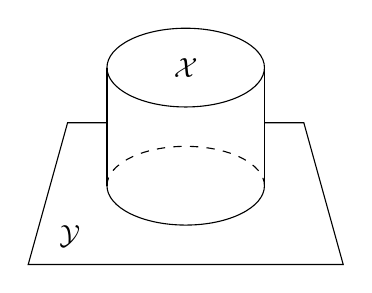
\begin{tikzpicture}[baseline=(O)]
	\draw (1, 1.5) ellipse[x radius=1, y radius=0.5] node {$\mathcal{X}$};
	\draw (0, 0) arc[start angle=180, end angle=360, x radius=1, y radius=0.5];
	\draw[dashed] (0, 0) arc[start angle=180, end angle=0, x radius=1, y radius=0.5];
	\draw (2, 1.5) -- (2, 0);
	\draw (0, 1.5) -- (0, 0);
	\draw (0, 0.8) -- (-0.5, 0.8) -- (-1, -1) node[xshift=1.5em,  yshift=1em] {$\mathcal{Y}$} -- (3, -1) -- (2.5, 0.8) -- (2, 0.8);
	\coordinate (O) at (0, 0.5);
\end{tikzpicture} \quad
	\Cone_{\mathrm{top}}(F) = 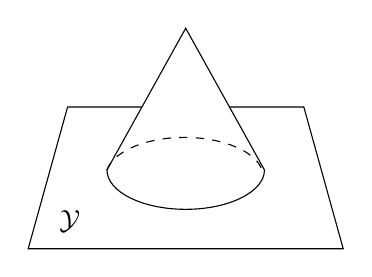
\begin{tikzpicture}[baseline=(O)]
	\draw (0, 0.8) -- (-0.5, 0.8) -- (-1, -1) node[xshift=1.5em,  yshift=1em] {$\mathcal{Y}$} -- (3, -1) -- (2.5, 0.8) --cycle;
	\filldraw[fill=white] (1, 1.8) -- (0, 0) arc[start angle=180, end angle=360, x radius=1, y radius=0.5] --cycle;
	\draw[dashed] (0, 0) arc[start angle=170, end angle=10, x radius=1, y radius=0.5];
	\coordinate (O) at (0, 0.5);
\end{tikzpicture}\]

单纯形集是剖析拓扑空间的一种具体手段. 稍加精确地说, 定理 \ref{prop:geom-Sing-adjunction} 给出伴随对
\[\begin{tikzcd}
	{|\cdot|}: \cate{sSet} \arrow[shift left, r] & \cate{Top}: \mathrm{Sing}, \arrow[shift left, l]
\end{tikzcd}\]
而且两端在某种精确意义下实现相互等价的同伦理论; 若以 $\cate{CGHaus}$ 代替 $\cate{Top}$, 前述构造同样适用. 我们现在着手将先前的讨论翻译到 $\cate{sSet}$ 中. 为此不妨就假定
\[ \mathcal{X} = |X|, \quad \mathcal{Y} = |Y|, \quad F = |f|: |X| \to |Y|, \]
其中 $f: X \to Y$ 是 $\cate{sSet}$ 的态射. 就单纯形集的立场, 映射锥比映射柱更容易解释. 我们先从 $\mathcal{X}$ 的锥 $\Cone_{\mathrm{top}}(\mathcal{X}) := \Cone_{\mathrm{top}}(\identity_{\mathcal{X}})$ 切入. 在 $\mathcal{X} = |X|$ 的前提下, $\Cone_{\mathrm{top}}(\mathcal{X}) \simeq |X^{\lhd}| \simeq |X^{\rhd}|$ (例 \ref{eg:cone-realization}). 以下将聚焦于 $X$ 的左锥 $X^{\lhd} = \Delta^0 \star X$ 和对应的链复形.
\index{danchunxingji!锥 (cone)}

对任意单纯形集 $Z$, 其中的非退化 $n$-单纯形构成集合 $Z^{\mathrm{nd}}_n$. 记 $\{\mathrm{pt}\} = (\Delta^0)_0 = (\Delta^0)^{\mathrm{nd}}_0$. 命题 \ref{prop:join-nd} 或拓扑直观表明
\begin{equation}\label{eqn:Cone-X-aux1}
	(\Delta^0 \star X)^{\mathrm{nd}}_n = \begin{cases}
		X^{\mathrm{nd}}_n \sqcup \left( \{ \mathrm{pt} \} \times X^{\mathrm{nd}}_{n-1} \right), & n > 0 \\
		\{\mathrm{pt}\} \sqcup X_0, & n = 0.
	\end{cases}
\end{equation}

代入 \eqref{eqn:join-formulas} 和其上讨论的一般公式, 可见当 $n \geq 1$ 时 $d_i: (\Delta^0 \star X)_n \to (\Delta^0 \star X)_{n-1}$ 在子集 $\{\mathrm{pt}\} \times X_{n-1}$ 和 $X_n$ 上的限制是
\begin{equation}\label{eqn:Cone-X-aux2}\begin{gathered}
	\begin{tikzcd}[column sep=small,
		/tikz/execute at end picture={
			\node [rectangle, draw, fit=(A) (B)] {};
			\node at ($(A)!.5!(C) + (0, 0.8)$) {$1 \leq i \leq n$};
		}]
		|[alias=A]| \{\mathrm{pt}\} \times X_{n-1} \arrow[d, "{\identity \times d_{i-1}}"'] & |[alias=C]| X_n \arrow[d, "{d_i}"] \\
		\{\mathrm{pt}\} \times X_{n-2} & |[alias=B]| X_{n-1}
	\end{tikzcd} \quad
	\begin{tikzcd}[column sep=small,
		/tikz/execute at end picture={
			\node [rectangle, draw, fit=(A) (B)] {};
			\node at ($(A)!.5!(C) + (0, 0.8)$) {$i=0$};
		}]
		|[alias=A]| \{\mathrm{pt}\} \times X_{n-1} \arrow[rd, "{\mathrm{pr}_2}"] & |[alias=C]| X_n \arrow[d, "{d_0}"] \\
		\{\mathrm{pt}\} \times X_{n-2} & |[alias=B]| X_{n-1}
	\end{tikzcd}
\end{gathered}\end{equation}
当 $n=1$ 时, 上式的 $\{\mathrm{pt}\} \times X_{n-2}$ 应理解为 $\{\mathrm{pt}\}$.

由于我们的目标是链复形, 下一步是将问题通过定义 \ref{def:free-simplicial-Ab} 的函子 $\Z(\cdot)$ 作线性化, 再以 Dold--Kan 对应过渡到链复形
\begin{equation*}
	\mathrm{N}(\Z X^{\lhd}) \simeq \mathrm{C}(\Z X^{\lhd}) \big/ \text{退化部分} \quad \text{(命题 \ref{prop:Dold-Kan-v})};
\end{equation*}
既然 $\mathrm{C}(\Z X^{\lhd})$ 的链复形结构来自 $\partial_n := \sum_{i=0}^n (-1)^i d_i$, 结合 \eqref{eqn:Cone-X-aux1}, \eqref{eqn:Cone-X-aux2} 连同注记 \ref{rem:cone-chain} 对 $\Cone(\identity_{\mathrm{N}X})$ 的描述, 可得链复形的短正合列
\[ 0 \to \underbracket{\Z\{\mathrm{pt}\}}_{\text{零次项}} \to \mathrm{N}(\Z X^{\lhd}) \to \Cone(\identity_{\mathrm{N}X}) \to 0. \]

其次, 函子 $|\cdot|$ 和 $\mathrm{N}$ 保推出图表, 这是因为它们分别是左伴随以及等价, 而推出图表在拓扑中的意义是黏合. 因此若对 $f: X \to Y$ 定义
\begin{equation*}
	\Cone_{\mathrm{s}}(f) := X^{\lhd} \dsqcup{X, f} Y,	
\end{equation*}
则有
\[\begin{tikzcd}
	\mathcal{X} \arrow[d, "F"'] \arrow[r, "{\text{底部}}"] & \Cone_{\mathrm{top}}(\mathcal{X}) \arrow[d] \\
	\mathcal{Y} \arrow[r] & \Cone_{\mathrm{top}}(F) \arrow[phantom, lu, "\boxplus" description]
\end{tikzcd} \xleftarrow{|\cdot|} \begin{tikzcd}
	X \arrow[d, "f"'] \arrow[r, "\text{典范}"] & X^{\lhd} \arrow[d] \\
	Y \arrow[r] & \Cone_{\mathrm{s}}(f) \arrow[phantom, lu, "\boxplus" description]
\end{tikzcd} \xrightarrow{\mathrm{N}} \begin{tikzcd}
	\mathrm{N}X \arrow[d, "{\mathrm{N}f}"'] \arrow[r] & \mathrm{N}X^{\lhd} \arrow[d] \\
	\mathrm{N}Y \arrow[r] & \mathrm{N}\Cone_{\mathrm{s}}(f) \arrow[phantom, lu, "\boxplus" description]
\end{tikzcd}\]
这一系列操作提示 $\Cone_{\mathrm{top}}(F)$ 的线性代数化身应当是 $\mathrm{N}\Cone_{\mathrm{s}}(f)$.

\begin{proposition}\label{prop:Cone-comparison}
	\index{yingshezhui}
	符号同上, 我们有链复形的典范短正合列
	\[ 0 \to \underbracket{\Z\{\mathrm{pt}\}}_{\text{零次项}} \to \mathrm{N}\Cone_{\mathrm{s}}(f) \to \Cone(\mathrm{N}f) \to 0. \]
\end{proposition}
\begin{proof}
	推出不触及 $\mathrm{N}X^{\lhd}$ 的子链复形 $\Z\{\mathrm{pt}\}$ (对应锥的顶点), 而它将 $n$ 次项的所有 $X_n$ 换成 $Y_n$, 并将 \eqref{eqn:Cone-X-aux2} 的投影 $\mathrm{pr}_2$ 换成 $f_{n-1} \mathrm{pr}_2$. 因此在商 $\Cone(\identity_{\mathrm{N}X})$ 的层次, 推出的产物无非是 $\Cone(\mathrm{N}f)$; 参阅注记 \ref{rem:cone-chain}.
\end{proof}

\begin{remark}
	映射柱 $\Cyl_{\mathrm{top}}(F)$ 及其链复形版本也可以作类似的会通, 而且此时不必再对顶点的贡献取商. 不过由于映射柱涉及单纯形集的乘积, 而 $\mathrm{N}$ 并非幺半函子, 所以拓扑学中一般是通过 CW 复形而非单纯形集来作解释, 乘积在 CW 复形的世界中更容易操作.
\end{remark}

综上, 链复形的映射锥是来自单纯形集 (或拓扑) 的映射锥对一份 $\Z$ 的商, 这份 $\Z$ 来自锥的顶点 $\mathrm{pt}$. 在链复形的研究中, 映射锥的主要意义是任何映射 $\phi: A \to B$ 都拓展为列:
\begin{equation}\label{eqn:cofiber-comparison-A}
	A \xrightarrow{\phi} B \to \Cone(\phi) \to A[-1] \xrightarrow{-f[-1]} B[-1] \to \cdots
\end{equation}

在拓扑情境下, 对应到 $\Cone(\phi) \to A[-1]$ 的映射是将 $\Cone_{\mathrm{top}}(F)$ 的底 $\mathcal{Y}$ 缩为一点, 收缩的产物记为 $S\mathcal{X}$; 这与 $\mathcal{Y}$ 无关 (见下图), 给出函子 $S$. 对应的映射列如
\begin{equation*}
	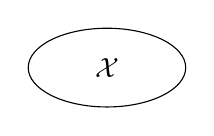
\begin{tikzpicture}[baseline=(O)]
		\draw (1, 0) ellipse[x radius=1, y radius=0.5] node {$\mathcal{X}$};
		\coordinate (O) at (0, 0);
	\end{tikzpicture}
	\xrightarrow{F}
	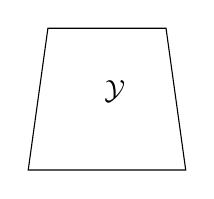
\begin{tikzpicture}[baseline=(O), xscale=0.5]
		\draw (0, 0.8) -- (-0.5, 0.8) -- (-1, -1) -- (3, -1) -- (2.5, 0.8) --cycle;
		\node at (1.2, 0) {$\mathcal{Y}$};
		\coordinate (O) at (0, 0.5);
	\end{tikzpicture}
	\xrightarrow{\text{嵌入}}
	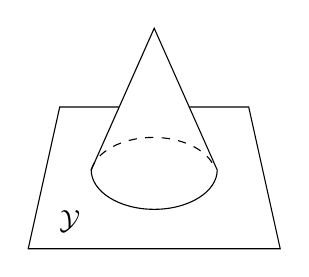
\begin{tikzpicture}[baseline=(O), xscale=0.8]
		\draw (0, 0.8) -- (-0.5, 0.8) -- (-1, -1) node[xshift=1.5em,  yshift=1em] {$\mathcal{Y}$} -- (3, -1) -- (2.5, 0.8) --cycle;
		\filldraw[fill=white] (1, 1.8) -- (0, 0) arc[start angle=180, end angle=360, x radius=1, y radius=0.5] --cycle;
		\draw[dashed] (0, 0) arc[start angle=170, end angle=10, x radius=1, y radius=0.5];
		\coordinate (O) at (0, 0.5);
	\end{tikzpicture}
	\xrightarrow{\text{缩}}
	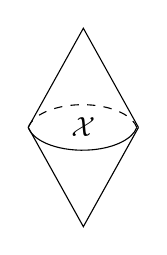
\begin{tikzpicture}[baseline=(O), xscale=0.7, yscale=0.7]
		\draw (2, 0) -- (1, 1.8) -- (0, 0);
		\draw[dashed] (0, 0) arc[start angle=170, end angle=10, x radius=1, y radius=0.5];
		\draw (0, 0) arc[start angle=190, end angle=350, x radius=1, y radius=0.5];
		\node at (1, 0) {$\mathcal{X}$};
		\draw (0, 0) -- (1, -1.8) -- (2, 0);
		\coordinate (O) at (0, 0.5);
	\end{tikzpicture}
	\to \cdots
\end{equation*}
称之为 $f$ 生成的\emph{上纤维列} (精确地说, 不带基点的版本). 若在 $\cate{sSet}$ 中操作, 对相应的列取链复形, 得到的大致是 \eqref{eqn:cofiber-comparison-A}. 之所以说``大致'', 缘由在于:
\begin{itemize}
	\item 映射 $S\mathcal{X} \to S\mathcal{Y}$ 不能单纯地取为 $S(F)$, 而须适当地翻转垂直坐标, 这在线性代数的层次对应到 \eqref{eqn:cofiber-comparison-A} 中的 $-f[-1]$; 详见拓扑学相关教材.
	\item 如命题 \ref{prop:Cone-comparison} 所见, 各种链复形包含多余的 $\Z$, 对应到 $\Cone_{\mathrm{top}}(F)$ 和 $S\mathcal{X}$ 等空间的顶点. 拓扑学中摆脱这些问题的方式是考虑带基点的空间, 然后在锥的拓扑构造中缩掉和基点相连的部分.
\end{itemize}

倘若暂时略去一切细节, 大而化之地说, 则 \S\ref{sec:derived-cat} 建立的导出范畴理论 (取 $\mathcal{A} = \cate{Ab}$) 也可视为同伦论\footnote{应当说是稳定同伦论, 因为链复形容许有负次项.}的一种略为粗糙的``线性化''.

由于相关问题涉及愈来愈多的拓扑学思想和方法, 为免离题万里, 我们就此打住.

\begin{Exercises}
	\item 证明对于任何范畴 $\mathcal{C}$, 例 \ref{eg:const-simplicial} 的构造 $C \mapsto \mathrm{const}(C)$ 给出全忠实函子 $\mathcal{C} \to \cate{s}\mathcal{C}$.
	
	\item 设 $X$ 是单纯形集, $x \in X_n$. 证明存在数列 $j_1 < \cdots < j_h$ 和一个非退化单纯形 $y$ 使得 $x = s_{j_h} \cdots s_{j_1} (y)$, 而且 $y$ 唯一.
	
	\begin{hint}
		难点在唯一性. 设 $Sy = x = S' y'$, 其中 $S$ 和 $S'$ 都具有断言中的形式, 则可取一系列面态射的合成 $D$ 使得 $y = DS y = DS' y'$; 将 $DS'$ 转换成 $\tilde{S}'\tilde{D}$ 的形式 (符号不言自明), 则 $y$ 非退化蕴涵 $\tilde{S}' = \identity$, 故 $y' = \tilde{D}y$. 运用对称性来推导 $y = y'$ 和 $\tilde{D} = \identity$.
	\end{hint}
	
	\item 说明在 $\cate{sSet}$ 中有如下图表, 上下两半分别交换 ($0 \leq i < j \leq n$):
	\[\begin{tikzcd}
		\Delta^{n-2} \arrow[d, "{\iota_{i < j}}"'] \arrow[r, "{\mathrm{d}^{j-1}}"] & \Delta^{n-1} \arrow[d, "\iota_i"] \arrow[rd, "{\mathrm{d}^i}"] & \\
		\bigsqcup_{0 \leq i' < j' \leq n} \Delta^{n-2} \arrow[shift left, r] \arrow[shift right, r] & \bigsqcup_{i' = 0}^n \Delta^{n-1} \arrow[r] & \partial \Delta^n \\
		\Delta^{n-2} \arrow[u, "{\iota_{i < j}}"] \arrow[r, "{\mathrm{d}^i}"'] & \Delta^{n-1} \arrow[u, "\iota_j"'] \arrow[ru, "{\mathrm{d}^j}"'] &
	\end{tikzcd}\]
	其中 $\bigsqcup$ 是在 $\cate{sSet} = \cate{Set}^{\simpDelta^{\opp}}$ 中逐项取的, 而 $\iota_{i < j}$ (或 $\iota_i$) 意谓向第 $i < j$ (或第 $i$) 项的嵌入; 中段的各个箭头由此交换性刻画. 进一步说明中间段是余等化子.
	
	类似地, 说明对所有 $0 \leq k \leq n$ 也同样有
	\[\begin{tikzcd}
		\Delta^{n-2} \arrow[d, "{\iota_{i < j}}"'] \arrow[r, "{\mathrm{d}^{j-1}}"] & \Delta^{n-1} \arrow[d, "\iota_i"] \arrow[rd, "{\mathrm{d}^i}"] & \\
		\bigsqcup_{\substack{0 \leq i' < j' \leq n \\ i', j' \neq k}} \Delta^{n-2} \arrow[shift left, r] \arrow[shift right, r] & \bigsqcup_{\substack{0 \leq i' \leq n \\ i' \neq k}} \Delta^{n-1} \arrow[r] & \Lambda^n_k \\
		\Delta^{n-2} \arrow[u, "{\iota_{i < j}}"] \arrow[r, "{\mathrm{d}^i}"'] & \Delta^{n-1} \arrow[u, "\iota_j"'] \arrow[ru, "{\mathrm{d}^j}"'] &
	\end{tikzcd}\]
	其中间段是余等化子, 要求 $i, j \neq k$. 试说明这些余等化子的拓扑意涵.
	
	\item 验证定义 \ref{def:simplicial-join} 的统联运算 $\star$ 有以下性质.
	\begin{enumerate}[(i)]
		\item 单纯形集对 $\star$ 自然地成为幺半范畴, 以取常值 $\emptyset$ 的空单纯形集为幺对象.
		\item 注记 \ref{rem:simpDelta-order-reversal} 的倒序对偶性给出 $\cate{sSet}$ 的自同构, 暂且记为 $X \mapsto \hat{X}$. 说明 $(X \star Y)^{\wedge} \simeq \hat{Y} \star \hat{X}$.
		\item 验证 $\Delta^p \star \Delta^q \simeq \Delta^{p+q+1}$.
	\end{enumerate}

	\item 说明精确到典范同胚, 对单纯形集取倒序对偶不改变几何实现.
	\begin{hint}
		从 $\Delta^n$ 的情形起步.
	\end{hint}

	\item 验证例 \ref{eg:cone-realization} 的断言.

	\item 设 $\mathcal{C}$ 和 $\mathcal{C}'$ 为范畴. 定义范畴 $\mathcal{C} \star \mathcal{C}'$ 如下:
	\begin{align*}
		\Obj(\mathcal{C} \star \mathcal{C}') & := \Obj(\mathcal{C}) \sqcup \Obj(\mathcal{C}'), \\
		\Hom_{\mathcal{C} \star \mathcal{C}'}(X, Y) & := \begin{cases}
			\Hom_{\mathcal{C}}(X, Y), & X, Y \in \Obj(\mathcal{C}) \\
			\Hom_{\mathcal{C}'}(X, Y), & X, Y \in \Obj(\mathcal{C}'), \\
			\text{独点集}, & X \in \Obj(\mathcal{C}), \; Y \in \Obj(\mathcal{C}'), \\
			\emptyset, & X \in \Obj(\mathcal{C}'), \; Y \in \Obj(\mathcal{C}).
		\end{cases}
	\end{align*}
	态射的合成与恒等态射有自明的定义. 证明单纯形集的统联运算 $\star$ 和例 \ref{eg:nerve-cat} 的脉函子有以下关系
	\[ \mathrm{N}(\mathcal{C}) \star \mathrm{N}(\mathcal{C}') \simeq \mathrm{N}(\mathcal{C} \star \mathcal{C}'). \]

	\item 为等式 \eqref{eqn:shuffle-sign-0} 和 \eqref{eqn:shuffle-sign-1} 给出较为详细的证明.
	
	\item 对任意范畴中的单纯形对象 $X$, 定义称为移位的单纯形对象 $\mathrm{Déc}_0 X$ 和 $\mathrm{Déc}^0 X$ 使得 $(\mathrm{Déc}_0 X)_n = (\mathrm{Déc}^0 X)_n = X_{n+1}$,
	\begin{gather*}
		d^{\mathrm{Déc}_0 X, n}_i = d^{X, n+1}_i, \quad s^{\mathrm{Déc}_0 X, n}_j = s^{X, n+1}_j, \\
		d^{\mathrm{Déc}^0 X, n}_i = d^{X, n+1}_{i+1}, \quad
		s^{\mathrm{Déc}^0 X, n}_j = s^{X, n+1}_{j+1}.
	\end{gather*}
	说明这是良定义的, 两者通过倒序对偶相联系 (注记 \ref{rem:simpDelta-order-reversal}), 而且对于加性范畴有 $\mathrm{C}(\mathrm{Déc}^0 X) = \mathrm{C}(X)[1]$ (参阅注记 \ref{rem:chain-cplx-translation}).
	\index{danchunxingduixiang!移位 (décalage)}
	\index[sym1]{Dec@$\mathrm{Déc}_0 X, \mathrm{Déc}^0 X$}

	\item 承上题, 说明 $d_0: X_1 \to X_0$ (或 $d_1: X_1 \to X_0$) 使 $\mathrm{Déc}_0 X$ (或 $\mathrm{Déc}^0 X$) 增广, 以 $X_0$ 为其 $-1$ 次项. 进一步说明在增广之后 $\mathrm{Déc}_0 X$ 右可缩, $\mathrm{Déc}^0 X$ 左可缩; 见定义 \ref{def:contractible-aug}.
	\begin{hint}
		处理 $\mathrm{Déc}_0 X$ 即可. 取 $k_{n-1} := s_n: X_n \to X_{n+1}$.
	\end{hint}

	\item 证明小范畴 $\mathcal{C}$ 是广群 (定义: 所有态射皆可逆) 当且仅当 $\mathrm{N}\mathcal{C}$ 具有以下条件: 对所有 $n \in \Z_{\geq 0}$ 和 $0 \leq i \leq n$, 任何态射 $\Lambda^n_i \to \mathrm{N}\mathcal{C}$ 都可以延拓为 $\Delta^n \to \mathrm{N}\mathcal{C}$, 不要求唯一性; 满足此延拓条件的单纯形集称为 Kan 复形.

	\item 延续例 \ref{eg:classifying-space-std-cplx} 的讨论, 说明正规化复形 $\overline{\mathsf{L}}$ (翻转为链复形) 同构于 $\mathrm{N}(\Bbbk\mathrm{E}\Gamma)$.
	\begin{hint}
		先以命题 \ref{prop:Dold-Kan-v} 将 $\mathrm{N}(X)$ 等同于 $\mathrm{C}(X)$ 的商.
	\end{hint}
	
	\item 设 $\Gamma$ 为幺半群. 记 $\cated{Set}\Gamma$ 为全体右 $\Gamma$-小集形成的范畴.
	\begin{enumerate}[(i)]
		\item 明确描述自由--忘却伴随对
		\[\begin{tikzcd}
			\mathrm{F}: \cate{Set} \arrow[shift left, r] & \cated{Set}\Gamma \arrow[shift left, l]: U
		\end{tikzcd}\]
		和对应的单位态射和余单位态射. 说明对应的单子 $T$ 将 $\cated{Set}\Gamma$ 等同于 $\cate{Set}^T$.
		
		\begin{hint}
			函子 $\mathrm{F}$ 映集合 $X$ 为 $X \times \Gamma$, 其中 $\Gamma$ 以右乘作用于第二个分量. 单位态射是 $x \mapsto (x, 1)$ 而余单位是作用映射.
		\end{hint}
		\item 对每个右 $\Gamma$-集 $X$ 描述 $\cated{Set}\Gamma$ 中对应的单纯形对象 $\mathrm{Bar}(X)$ (例 \ref{eg:bar-adjunction}, 例 \ref{eg:bar-comonad}).
		\item 取独点集 $X = \{\mathrm{pt}\}$, 赋予平凡右 $\Gamma$-作用. 说明对应的单纯形对象同构于例 \ref{eg:classifying-space} 介绍的 $\mathrm{E}\Gamma$, 后者通过每个 $(\mathrm{E}\Gamma)_n$ 上的右 $\Gamma$-作用成为 $\cated{Set}\Gamma$ 中的单纯形对象.
	\end{enumerate}

	\item 选定群 $\Gamma$. 在例 \ref{eg:HH-comonad} 中取群代数 $R = \Bbbk[\Gamma]$, 取 $M$ 为平凡 $\Gamma$-模 $\Bbbk$ (例 \ref{eg:trivial-G-mod}). 说明对应的 $\epsilon_{\Bbbk}: \mathrm{C}(\mathrm{Bar}(\Bbbk)) \to \Bbbk$ 同构于命题 \ref{prop:trivial-mod-resolution} 的解消 $\mathsf{L} = (\mathsf{L}_n, \partial'_n)_n \to \Bbbk$.
	\begin{hint}
		应用 \eqref{eqn:L-basis-partial}.
	\end{hint}

	\item 取交换环 $\Bbbk$ 和 $\mathcal{A} = \Bbbk\dcate{Mod}$, $\otimes = \otimes_{\Bbbk}$. 设 $\Gamma$ 为群, 考虑例 \ref{eg:classifying-contractible} 中的单纯形对象 $\Bbbk\mathrm{E}\Gamma$, 在 Alexander--Whitney 映射的定义 \ref{def:Eilenberg-Zilber} 中代入 $X := \Bbbk\mathrm{E}\Gamma \boxtimes \Bbbk\mathrm{E}\Gamma$, 然后考虑态射
	\[ \mathrm{C}(\Bbbk\mathrm{E}\Gamma) \to \mathrm{C}(\underbracket{\Bbbk\mathrm{E}\Gamma \otimes \Bbbk\mathrm{E}\Gamma}_{\simeq \Bbbk(\mathrm{E}\Gamma \times \mathrm{E}\Gamma)}) \xrightarrow{\overline{\mathrm{AW}}} \mathrm{C}(\Bbbk\mathrm{E}\Gamma) \otimes \mathrm{C}(\Bbbk\mathrm{E}\Gamma), \]
	第一段由单纯形集的对角嵌入 $\mathrm{E}\Gamma \to \mathrm{E}\Gamma \times \mathrm{E}\Gamma$ 诱导; 鉴于例 \ref{eg:classifying-space-std-cplx}, 其合成也相当于链复形的态射
	\[ \mathsf{L} \to \mathsf{L} \otimes \mathsf{L}. \]
	试由此诠释定义群上同调的杯积时用过的态射 $\Delta: \mathsf{L} \to \mathsf{L} \otimes \mathsf{L}$; 见引理 \ref {prop:cup-resolution} (ii).
	
	\begin{hint}
		代入 $\overline{\mathrm{AW}}$ 的定义可见合成态射的 $(p, q)$ 分量和引理 \ref {prop:cup-resolution} (ii) 差一个 $(-1)^{pq}$. 差异缘于该处探讨的是 $(\mathsf{L}_n, \partial_n)_n$ 而例 \ref{eg:classifying-space-std-cplx} 则取 $(\mathsf{L}_n, \partial'_n)_n$. 两者在单纯形集 $\mathrm{E}\Gamma$ 的层次差一个倒序 (注记 \ref{rem:simpDelta-order-reversal}); 留意到倒序对偶性调换 $\lambda^n_p$ 和 $\rho^n_q$ 在 $\overline{\mathrm{AW}}$ 中的角色, 或者说是调换两份 $\mathrm{C}(\Bbbk\mathrm{E}\Gamma)$.
	\end{hint}

	\item 考虑范畴 $\mathcal{D}$ 上的余单子 $(L, \delta, \epsilon)$. 对任意 $\mathcal{M} \in \Obj(\mathcal{D})$, 若 $\epsilon_{\mathcal{M}}: L\mathcal{M} \to \mathcal{M}$ 有右逆 $f: \mathcal{M} \to L\mathcal{M}$, 则称 $\mathcal{M}$ 是 \emph{$L$-投射}对象. 对偶地, 从范畴 $\mathcal{C}$ 上的单子 $(T, \mu, \eta)$ 可定义何谓 $\mathcal{C}$ 的 \emph{$T$-内射}对象.
	
	基于对偶性, 以下主要讨论 $L$-投射的概念. 按照例 \ref{eg:monad-simplicial} 的方法在 $\End(\mathcal{D})$ 中得到增广单纯形对象 $(L^{n+1})_{n \geq -1}$ (符号中省略 $d_i$, $s_j$ 等资料). 给定 $L$-投射的 $\mathcal{M}$ 和相应的 $f$, 定义
	\[ k_n := L^{n+1} f : L^{n+1} \mathcal{M} \to L^{n+2} \mathcal{M}, \quad n \geq -1. \]
	证明这使增广单纯形对象 $(L^{n+1} \mathcal{M})_{n \geq -1}$ 右可缩 (定义 \ref{def:contractible-aug}).

	\begin{hint}
		已知 $\epsilon_{\mathcal{M}} k_{-1} = \epsilon_{\mathcal{M}} f = \identity_{\mathcal{M}}$, 两边同取 $L^{n+1}$ 给出 $d_{n+1} k_n = \identity_{X_n}$, 而函子性确保
		\[\begin{tikzcd}
			L\mathcal{M} \arrow[r, "Lf"] \arrow[d, "{\epsilon_{\mathcal{M}}}"'] & L^2 \mathcal{M} \arrow[d, "{\epsilon_{L\mathcal{M}}}"] \\
			\mathcal{M} \arrow[r, "f"'] & L\mathcal{M}
		\end{tikzcd} \quad\text{交换, 亦即}\; d_0 k_0 = 	f\epsilon_{\mathcal{M}} = k_{-1} \epsilon_{\mathcal{M}}; \]
		以 $L^{n-i}f$ 代 $f$, 再对相应的图表取 $L^i$, 同理可得 $d_i k_n = k_{n-1} d_i$ 对 $0 \leq i \leq n$ 成立.
	\end{hint}

	\item 对于环 $R$, 自由--忘却伴随对 $\cate{Set} \leftrightarrows R\dcate{Mod}$ 确定 $R\dcate{Mod}$ 上的余单子 $L$. 证明一个左 $R$-模是 $L$-投射的当且仅当它是投射模.

	\item 考虑伴随对
	$\begin{tikzcd}
		F: \mathcal{C} \arrow[shift left, r] & \mathcal{D}: G \arrow[shift left, l]
	\end{tikzcd}$
	和 $\End(\mathcal{D})$ 上相应的余单子 $(L, \delta, \epsilon) = (FG, F\eta G, \epsilon)$ (例 \ref{eg:adjunction-monad}). 证明形如 $F\mathcal{N}$ 的对象 ($\mathcal{N} \in \Obj(\mathcal{C})$) 总是 $L$-投射的. 作为推论, 对所有 $\mathcal{M} \in \Obj(\mathcal{D})$, 单纯形对象 $(L^{n+1} \mathcal{M})_{n \geq 0}$ 的每一项都是 $L$-投射对象.
	
	\begin{hint}
		取 $f = F\eta_{\mathcal{N}}: F(\mathcal{N}) \to FGF(\mathcal{N}) = L(F(\mathcal{N}))$, 则 $\epsilon_{F(\mathcal{N})} f = \identity_{F(\mathcal{N})}$ 不外是伴随对的标准性质.
	\end{hint}

	\item 仍考虑来自伴随对 $(F, G)$ 的余单子 $L$. 说明 $\mathcal{P} \in \Obj(\mathcal{D})$ 是 $L$-投射的当且仅当它有以下提升性质: 对 $\mathcal{D}$ 的任意态射 $\alpha: \mathcal{M}_1 \to \mathcal{M}_2$ 和 $\phi: \mathcal{P} \to \mathcal{M}_2$, 若 $G\alpha$ 有右逆, 则存在 $\beta: \mathcal{P} \to \mathcal{M}_1$ 使得 $\phi = \alpha\beta$.

	\begin{hint}
		对于``当''的方向, 对 $\alpha := \epsilon_{\mathcal{P}}: FG(\mathcal{P}) \to \mathcal{P}$ 和 $\phi := \identity$ 应用提升性质. 对于``仅当''方向, 首先解释在提升性质中可用 $FG(\mathcal{P})$ 代 $\mathcal{P}$, 然后以伴随性质说明 $\alpha_*: \Hom(FG(\mathcal{P}), \mathcal{M}_1) \to \Hom(FG(\mathcal{P}), \mathcal{M}_2)$ 满.
	\end{hint}

	\item 对任意交换环 $\Bbbk$ 和 $\Bbbk$-代数的同态 $S \to R$, 考虑伴随对
	\begin{equation*}\begin{tikzcd}[row sep=small]
		R \dotimes{S} (\cdot): S\dcate{Mod} \arrow[shift left, r] & R\dcate{Mod}: \text{忘却}, \arrow[shift left, l] \\
		\text{忘却}: R\dcate{Mod} \arrow[shift left, r] & S\dcate{Mod}: \Hom_S(R, \cdot) \arrow[shift left, l]
	\end{tikzcd}\end{equation*}
	由此分别得到 $R\dcate{Mod}$ 上的余单子 $L$ 和单子 $T$. 试以先前介绍的提升性质 (或其对偶) 给出一个左 $R$-模 $M$ 作为 $L$-投射 (或 $T$-内射) 对象的充要条件, 然后比较它和投射模 (或内射模) 的异同.
	
	在此基础上可以建立一套称为\emph{相对同调代数}的理论, 详见 \cite{Ho56}; 其特色是它仅考量在 $S$ 上分裂正合的 $R$-模正合列. 稍后的习题将探讨相对版本的 $\Tor$ 和 $\Ext$ 函子.
	\index{xiangduitongdiaodaishu@相对同调代数 (relative homological algebra)}

	\item 考虑 Abel 范畴之间的伴随对
	$\begin{tikzcd}
		F: \mathcal{C} \arrow[shift left, r] & \mathcal{D}: G \arrow[shift left, l]
	\end{tikzcd}$.
	对所有 $\mathcal{M} \in \Obj(\mathcal{D})$ 证明:
	\begin{enumerate}[(i)]
		\item 存在 $\cate{Ch}_{\geq 0}(\mathcal{D})$ 的对象 $\mathcal{P}_\bullet$ 连同态射 $\epsilon: \mathcal{P}_\bullet \to \mathcal{M}$, 使得
		\begin{compactitem}
			\item 每个 $\mathcal{P}_n$ 都是 $L$-投射的 ($n \geq 0$),
			\item $\cdots \to G\mathcal{P}_1 \to G\mathcal{P}_0 \to G\mathcal{M} \to 0$ 的恒等态射零伦 (换言之, 它是分裂正合复形).
		\end{compactitem}
		\begin{hint}
			应用命题 \ref{prop:bar-null-homotopic}.
		\end{hint}
		\item 给定任两组满足上述条件的态射 $\epsilon: \mathcal{P}_\bullet \to \mathcal{M}$ 和 $\epsilon': \mathcal{P}'_\bullet \to \mathcal{M}$, 存在同伦等价 $f: \mathcal{P} \to \mathcal{P}'$ 使得 $\epsilon' f = \epsilon$.
		\begin{hint}
			需要之前介绍的提升性质.
		\end{hint}
	\end{enumerate}

	\index{yudanzitongdiao@余单子同调 (cotriple homology)}
	\index{ganggouzao}
	\item (M.\ Barr, J.\ M.\ Beck) 设 $L$ 是范畴 $\mathcal{D}$ 上的余单子; 例 \ref{eg:monad-simplicial} 的构造在 $\mathcal{M} \in \Obj(\mathcal{D})$ 取值给出的单纯形对象记为 $\mathrm{Bar}(\mathcal{M})$. 对任意 Abel 范畴 $\mathcal{A}$ 和函子 $E: \mathcal{D} \to \mathcal{A}$, 定义 $(L, E)$ 的\emph{余单子同调}为 $\cate{Ch}_{\geq 0}(\mathcal{A})$ 的一族对象
	\[ \Hm^L_n(E; \mathcal{M}) := \Hm_n\left( \mathrm{C}(E\mathrm{Bar}(\mathcal{M})) \right), \quad n \in \Z_{\geq 0}, \]
	其中 $E\mathrm{Bar}(\mathcal{M})$ 代表对 $\mathrm{Bar}(\mathcal{M})$ 逐项地取 $E$. 对偶地, 若 $T$ 是范畴 $\mathcal{C}$ 上的单子, $F: \mathcal{C} \to \mathcal{A}$ 是映向 Abel 范畴的函子, 则同样能定义 $(T, F)$ 的\emph{单子上同调}在 $\mathcal{N} \in \Obj(\mathcal{C})$ 的取值, 不必赘言.

	\begin{enumerate}[(i)]
		\item 写下自然态射 $\Hm^L_0(E; \mathcal{M}) \to E\mathcal{M}$, 说明当 $\mathcal{M}$ 为 $L$-投射对象时此为同构.
		\item 设 $L$ 来自 Abel 范畴之间的伴随对 $(F, G)$, 而 $E$ 是加性函子. 证明若 $\mathcal{P}_\bullet \to \mathcal{M}$ 是 $\cate{Ch}_{\geq 0}(\mathcal{D})$ 的态射, 满足
		\begin{compactitem}
			\item 每个 $\mathcal{P}_n$ 都是 $L$-投射的 ($n \geq 0$),
			\item $\cdots \to G\mathcal{P}_1 \to G\mathcal{P}_0 \to G\mathcal{M} \to 0$ 的恒等态射零伦,
		\end{compactitem}
		则 $\Hm^L_n(E; \mathcal{M}) \simeq \Hm_n(E\mathcal{P}_\bullet)$. 因此, 余单子同调可以用合适的 $L$-投射解消来计算.
		\item 承继先前假设. 若 $\mathcal{D}$ 的态射 $\mathcal{M}' \to \mathcal{M} \to \mathcal{M}''$ 取 $G$ 之后是 $\mathcal{C}$ 的分裂短正合列, 则称之为 $G$-分裂短正合列. 证明 $G$-分裂短正合列自然地诱导 $\Hm^L_n(E; \cdot)$ 的长正合列.
	\end{enumerate}

	\index{Ext hanzi!相对 (relative)}
	\index{Tor hanzi!相对 (relative)}
	\item (G.\ Hochschild \cite{Ho56}) 对任意交换环 $\Bbbk$ 和 $\Bbbk$-代数的同态 $S \to R$, 考虑伴随对
	\[\begin{tikzcd}
		R \dotimes{S} (\cdot): S\dcate{Mod} \arrow[shift left, r] & R\dcate{Mod}: \text{忘却} \arrow[shift left, l]
	\end{tikzcd}\]
	在 $R\dcate{Mod}$ 上确定的余单子 $L$. 对右 $R$-模 $A$ 和左 $R$-模 $B$, $N$, 定义 $\Bbbk$-模
	\begin{align*}
		\Tor^{R|S}_n(A, N) & := \Hm^L_n\left( A \dotimes{R}(\cdot) ; N \right), \\
		\Ext_{R|S}^n(N, B) & := \Hm^L_n\left( \Hom_R(\cdot, B) ; N \right),
	\end{align*}
	此处 $\Hom_R(\cdot, B)$ 视为函子 $R\dcate{Mod} \to S\dcate{Mod}^{\opp}$. 它们称为相对 $\Tor$ 和相对 $\Ext$ 函子.
	\begin{enumerate}[(i)]
		\item 说明两者对每个变元皆有函子性. 试明确相应的链复形, 并说明
		\[ \Tor^{R|S}_0(A, N) \simeq A \dotimes{R} N, \quad \Ext_{R|S}^0(N, B) \simeq \Hom_R(N, B). \]
		
		\item 说明双函子 $\Tor^{R|S}_n$ 有类似于定理 \ref{prop:balanced-primer} 的``平衡''性质.\footnote{避谈 $\Ext_{R|S}^n$ 是因为它涉及单子上同调的概念, 此处不细说, 详阅参考文献.}
		
		\item 证明若 $I$ 是 $S$ 的双边理想而 $R = S/I$, 则当 $n > 0$ 时 $\Tor_n^{R|S} = 0 = \Ext^n_{R|S}$. 由此可见相对 $\Tor$ 和相对 $\Ext$ 不同于 \S\ref{sec:Ext-Tor} 的绝对版本.
		\begin{hint}
			此时 $L = \identity_{R\dcate{Mod}}$.
		\end{hint}
		
		\item 记 $R^e = R \dotimes{\Bbbk} R^{\opp}$. 证明 $\HHm_n(M) \simeq \Tor^{R^e|\Bbbk}_n(M, R)$ 而 $\HHm^n(M) \simeq \Ext_{R^e|\Bbbk}^n(R, M)$; 参见例 \ref{eg:HH-comonad}.
		\begin{hint}
			归结为说明 $\mathrm{C}(\mathrm{Bar}(R))_n = R \otimes R^{\otimes n} \otimes R$ 是 $L$-投射的 $R^e$-模.
		\end{hint}
	\end{enumerate}
\end{Exercises}